%%%%%%%%%%%%%%%%%%%%%%%%%%%%%%%%%%%%%%%%%%%%%%%%%%%%%%%%%%%%%%%%%%%%%%%%%%
%
% TRS - User Guide and Reference Manual -- LaTeX Source 
%
% $Id: trs.tex,v 1.5 2006/08/15 21:42:17 jeromel Exp $
%
% Author: LaTeX template by Thomas Ullrich
%         1st version by brian
%
%%%%%%%%%%%%%%%%%%%%%%%%%%%%%%%%%%%%%%%%%%%%%%%%%%%%%%%%%%%%%%%%%%%%%%%%%%
%
% $Log: trs.tex,v $
% Revision 1.5  2006/08/15 21:42:17  jeromel
% Fix rhic -> rhic.bnl.gov
%
% Revision 1.4  2000/01/11 23:18:37  lasiuk
% pdf and fancyheadings
%
% Revision 1.3  1999/01/24 20:58:59  lasiuk
% simple corrections
%
% Revision 1.2  1999/01/24 03:32:57  lasiuk
% update of manual
%
% Revision 1.1  1999/01/12 15:35:25  lasiuk
% Initial Revision
%
%
%%%%%%%%%%%%%%%%%%%%%%%%%%%%%%%%%%%%%%%%%%%%%%%%%%%%%%%%%%%%%%%%%%%%%%%%%%
\documentclass[twoside]{article}

\parindent 0pt
\parskip 6pt
\advance\textwidth by 80pt%
\advance\evensidemargin by -80pt%

\usepackage{graphicx}
\usepackage{psboxit}
\usepackage{color}
\usepackage{amsmath}
\usepackage{amssymb}
%\usepackage{fancyheadings}
\usepackage{fancyhdr}
\usepackage{times}
\usepackage{verbatim}
\usepackage{makeidx}
%\usepackage{subfigure}

\PScommands      % init boxit
\makeindex

%%%%%%%%%%%%%%%%%%%%%%%%%%%%%%%%%%%%%%%%%%%%%%%%%%%%%%%%%%%%%%%%%%%%
%
% Define header and footer style
%
%%%%%%%%%%%%%%%%%%%%%%%%%%%%%%%%%%%%%%%%%%%%%%%%%%%%%%%%%%%%%%%%%%%%
\pagestyle{fancyplain}
\rhead[\fancyplain{}{\bfseries\leftmark}]
      {\fancyplain{}{\bfseries\rightmark}}
\lhead[\fancyplain{}{\bfseries\rightmark}]
      {\fancyplain{}{\bfseries\leftmark}}
\rfoot[{}]{\fancyplain{}{\bfseries\thepage}}
\lfoot[\fancyplain{}{\bfseries\thepage}]{}
\cfoot{}

%%%%%%%%%%%%%%%%%%%%%%%%%%%%%%%%%%%%%%%%%%%%%%%%%%%%%%%%%%%%%%%%%%%%
%
% Typographic Conventions
%
%%%%%%%%%%%%%%%%%%%%%%%%%%%%%%%%%%%%%%%%%%%%%%%%%%%%%%%%%%%%%%%%%%%%
\newcommand{\name}[1]{\textsf{#1}}%  or class-, function-, package names
\newcommand{\comp}[1]{\texttt{#1}}%  computer font
\newcommand{\args}[1]{\textit{#1}}%   command arguments

%%%%%%%%%%%%%%%%%%%%%%%%%%%%%%%%%%%%%%%%%%%%%%%%%%%%%%%%%%%%%%%%%%%%
%
% Define multiline labels for class reference
%
%%%%%%%%%%%%%%%%%%%%%%%%%%%%%%%%%%%%%%%%%%%%%%%%%%%%%%%%%%%%%%%%%%%%
\newcommand{\entrylabel}[1]{\mbox{\textbf{{#1}}}\hfil}%
\newenvironment{entry}
{\begin{list}{}%
    {\renewcommand{\makelabel}{\entrylabel}%
     \setlength{\labelwidth}{90pt}%
     \setlength{\leftmargin}{\labelwidth}
     \advance\leftmargin by \labelsep%
      }%
    }%
  {\end{list}}

\newcommand{\Entrylabel}[1]%
{\raisebox{0pt}[1ex][0pt]{\makebox[\labelwidth][l]%
    {\parbox[t]{\labelwidth}{\hspace{0pt}\textbf{{#1}}}}}}
\newenvironment{Entry}%
{\renewcommand{\entrylabel}{\Entrylabel}\begin{entry}}%
  {\end{entry}}

\begin{document}

%%%%%%%%%%%%%%%%%%%%%%%%%%%%%%%%%%%%%%%%%%%%%%%%%%%%%%%%%%%%%%%%%%%%
%
%    Title page
%
%%%%%%%%%%%%%%%%%%%%%%%%%%%%%%%%%%%%%%%%%%%%%%%%%%%%%%%%%%%%%%%%%%%%
\begin{titlepage}
\pagestyle{empty}
\vspace*{-35mm}
\begin{center}
  \mbox{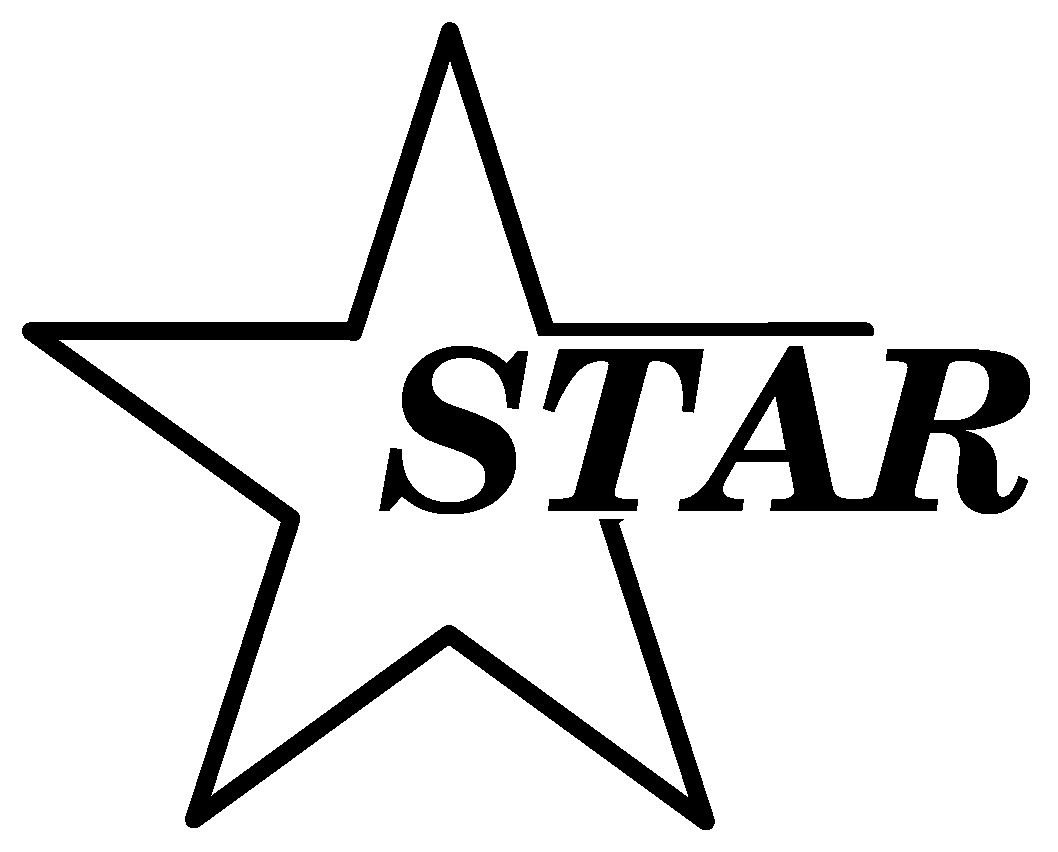
\includegraphics[width=2cm]{StarIcon.eps}}
  {\Large\bf Offline Library TRS Long Writeup}
  \hfill\mbox{}\\[3cm]
  \mbox{\includegraphics[width=\textwidth]{trsTitle.eps}}
  \hfill\mbox{}\\[3cm]
  {\LARGE User Guide and Reference Manual}\\[2cm]
  {\LARGE $ $Revision: 1.5 $ $}  \\[5mm] % replaced by cvs with current revision  
  {\LARGE $ $Date: 2006/08/15 21:42:17 $ $}  % replaced by cvs with current revision  
  \vfill
\end{center}
\cleardoublepage
\end{titlepage}
\pagenumbering{roman}

%%%%%%%%%%%%%%%%%%%%%%%%%%%%%%%%%%%%%%%%%%%%%%%%%%%%%%%%%%%%%%%%%%%%
%
%    Table of content
%
%%%%%%%%%%%%%%%%%%%%%%%%%%%%%%%%%%%%%%%%%%%%%%%%%%%%%%%%%%%%%%%%%%%%
\tableofcontents
\cleardoublepage

%%%%%%%%%%%%%%%%%%%%%%%%%%%%%%%%%%%%%%%%%%%%%%%%%%%%%%%%%%%%%%%%%%%%
%
%    User Guide
%
%%%%%%%%%%%%%%%%%%%%%%%%%%%%%%%%%%%%%%%%%%%%%%%%%%%%%%%%%%%%%%%%%%%%
\pagenumbering{arabic}
\part{User Guide}
\clearpage

\section{Philosophy and Motivation} \index{philosophy}
\label{Philosophy}

With the decision at the STAR collaboration meeting in January 1998
at LBNL that a migration to the C++ programming language and 
Object-Oriented (OO)
coding practices will be made, it was suggested that the TPC slow simulator
be the first package to be re-engineered using these techniques
and principles.  This project was to be a prototype for such future
developments within the collaboration, both in its design and structure.  
A requirements documents was quickly prepared after the meeting
and work began on simple design, prototyping, and evaluation of 
various commercial and public domain class libraries.

The result of these initial studies was the development of the 
StarClassLibrary\footnote{http://star.physics.yale.edu/SCL} 
\index{SCL} which drew on the developments of 
CLHEP\index{http://wwwinfo.cern.ch/lhc++/clhep/index.htm} \index{CLHEP} 
but relied heavily on the
ANSI \index{ANSI} standard\footnote{http://www.cyngus.com/misc/wp/nov97/} 
C++ Standard Library and specifically the Standard Template
Library or STL. \index{STL}  This library provides several
physics containers (three- and four- vectors) as well as matrices
random number generators, a system of units, etc.).  It was upon this
development that the \name{TPC Response Simulator} (\name{TRS}) was built.

The goal of re-engineering \name{TRS} was two-fold:
%%%%%%%%%%%%%%%%%%%%%%%%%%%%%%%%%%%%%%%%%%%%%%%%%%%%%%%%%%%%%%%%%%%%
\begin{itemize}
  \item generate an object-oriented package using C++ in the
    STAR computing environment.
  \item add detail and develop the simulation tools parallel to the
    commissioning schedule of the STAR TPC.
\end{itemize}
%%%%%%%%%%%%%%%%%%%%%%%%%%%%%%%%%%%%%%%%%%%%%%%%%%%%%%%%%%%%%%%%%%%%
In order to add flexibility to the package it was designed to
support two types of simulation from a single interface; that is,
a very detailed microscopic simulation of the processes occurring
in the STAR-TPC and a faster parameterized version which could be
used for large scale processing.  In order to do this the design
concentrated on isolating the physics
processes of interest and how the data could be stored in generic
data containers.  These ideas, as well as a preliminary class design
were drawn up in a design document\footnote{see http://www.rhic.bnl.gov/STAR/html/comp\_l/simu/TpcRespSim/src/ps/TrsDesign.ps} 
which was discussed at the STAR 
collaboration meeting in August 1998 at BNL.  This document was
the basis for the design and developments for the first version
of \name{TRS}.  This document is a report of these developments as well
as a guide for its use in its current form.

\section{Organization of the Manual}

This manual is a description of the \name{TPC Response Simulator} 
(\name{TRS}) package.  The first part of the manual is a {\bf User Guide} 
which describes the platform dependencies, package organization and
general description of the design and basic implementation of
the components within the package.  The subsequent parts make
up the {\bf Reference Manual} which is a detailed description of the
component classes of \name{TRS}.  This is broken into four different 
sections, the first two of which describe the generic data base
and coordinate classes used in the package, which are not necessarily
specific to TRS, but which are of interest to the general STAR
software environment and could be used in any software package.  If
these gain acceptance within the collaboration, they can be moved
to a more accessible location such as the \name{StarClassLibrary} 
\index{STAR Class Library}
The last two parts deal with the \name{TRS} specific classes which
are broken into two separate components---the {\bf containers}
and {\bf processes}.

\section{Platforms and Compilers} \index{compiler} \index{platform}
\label{platformsAndCompilers}

The \name{TPC Response Simulator} (\name{TRS}) was developed on
an HP \index{HP} workstation since HP currently provides the
closest ANSI \index{ANSI} compliant compiler and standard libraries.  However
the target platforms on which the code will ultimately
run are LINUX \index{Linux} and SUN \index{SUN}.  Red Hat LINUX 5.0
and higher versions provide very close to fully ANSI compliant compilers
with only exceptions\footnote{and some member functions of minimal
  importance in the STL.}
being not fully
supported.  The current SUN compiler (CC v4.2) however,
is far from compliant and the large scale use of macros populate
the code to allow for operation in a SOLARIS \index{SOLARIS} 
environment.  A modified standard C++ library from Object 
Space \index{Object Space} (v2.0.2) was created in order to make up for
the vendor short-comings.  This library is currently available
for distribution from the STAR CVS \index{CVS} repository.  
It is foreseen that the
new SUN compiler (CC v5.0) which is scheduled for release in
March of 1999 should large solve many of the current problems
and inconveniences of the SUN compiler.

\name{TRS} has been tested and the example programs that 
utilize the \name{TRS} classes currently compile on the following 
platforms:
%%%%%%%%%%%%%%%%%%%%%%%%%%%%%%%%%%%%%%%%%%%%%%%%%%%%%%%%%%%%%%%%%%%%
\begin{enumerate}
\item HP-UX 10.20: \index{HP-UX}
  \begin{itemize}
    \item aCC A.01.06 or higher versions. The standard library
      supplied from the vendor is the basis of most other libraries
      in the industry. \index{aCC (HP compiler)}
  \end{itemize}
\item Red Hat Linux 5.0 or higher versions: \index{Linux}
  \begin{itemize}
    \item egcs 1.0.2 (g++).
  \end{itemize}
\item Solaris 2.4--2.6: \index{Solaris}
  \begin{itemize}
    \item CC 4.2 and Object Space 2.0.2 modified. \index{Object Space}
  \end{itemize}
\end{enumerate}
%%%%%%%%%%%%%%%%%%%%%%%%%%%%%%%%%%%%%%%%%%%%%%%%%%%%%%%%%%%%%%%%%%%%%%%
Tests with Visual C++ 5.0 have not been attempted since the
StarClassLibrary (SCL) \index{SCL} does
not currently build due to the lack of support of \index{Visual C++}
templated member functions and a broken overloading mechanism.  It
is hoped that this will be addressed with v6.0 which has been released
(but not tested).  In the interim, non-templated container classes
have been written and incorporated into the\name{SCL}, so that this
should now be possible.
No efforts have been spent to write, port, or adapt the code
to SGI-IRIX \index{Irix} 
nor IBM-AIX and such developments are not foreseen  unless there is
significant user demand. \index{Irix} \index{AIX}

\section{Organization of the \name{TRS} Package}

All documentation, code, and header files of \name{TRS} are contained in
the {\bf CVS} repository at BNL in the \comp{\$STAR/StRoot} section
in a
directory named \name{./St\_trs\_Maker}.\footnote{To be changed to: 
        \name{StTrsMaker/}}.  
There are several subdirectories
in  which  the code is then distributed.  The header files as well
as the source code in contained in the \name{./include} and \name{./src}
directories respectively.  The \name{./local} directory contains the
necessary {\bf GNUMakefile}s in order to compile stand-alone shared
libraries such that code can be run outside the ROOT/STAR framework.
This was initially done to avoid the complications of the constantly
evolving STAR infrastructure, (i.e.~STAF/ROOT) \index{STAF} \index{ROOT}
however it has been retained in order to aid in parallel development
projects which require the use of some classes within \name{TRS}, but do
not necessarily require or warrant the use of the complete STAR 
infrastructure.  

Example programs as well as those to monitor and control the developments
within the \name{TRS} classes are contained in the directory \name{./examples}.
This directory also contains the necessary {\bf GNUMakefile}s for 
compilation.  To avoid confusion, both the \name{TRS} shared libraries and the
executables from the shared libraries are kept in a directory denoted by
the system architecture derived from the STAR environment
variable {\bf \$STAR\_SYS}.  Finally the documentation is stored in the
\name{./doc} directory.  This currently consists of this manual which
is written in \LaTeX.  A class browser which illustrates the function
prototypes, also used with the SCL is also a possibility in the future.
The developments that occur in TRS are kept on the STAR WWW \index{WWW}
page (see: http://www.rhic.bnl.gov/STAR/html/comp\_l/simu/TpcRespSim/src/Welcome.html).

All makefiles are especially written for the \name{GNU} make utility (gmake) 
and rely on
certain features only available therein. This is also the reason why we do not
follow the standard naming scheme but named them \name{GNUmakefile}. 
Note that these {\bf Makefile}s do not contain any hard-wired file names;
the dependencies are rather created on-the-fly at compile time.  The
libraries should also be generated from within the "official" STAR
{\bf Makefile}s.

\section{Requirements and Installation of TRS}  \index{Installing TRS} 
\index{requirements} 
\label{install}

The TPC Response Simulator (\name{TRS}) requires the Standard C++ Library,
including the STL \index{STL} as well as the STAR Class Library (SCL).
\name{TRS} was structured such that if the SCL will
compile and run on a system, so too will \name{TRS}.

\name{TRS} is part of the official STAR software distribution
and is therefore present in the actual STAR software releases.
If you want to install \name{TRS} locally on your machine you should
continue to read the following three sections which explains how to
obtain, compile and install the code.

\subsection{The source code} 

The \name{TPC Response Simulator} is under {\bf CVS} control at BNL.  It can
be accessed via \name{afs}: \index{afs} \index{CVS} \index{CVSROOT}
\begin{enumerate}
  \item Obtain an \name{afs} token: \comp{klog -cell rhic}.
  \item Make sure \comp{\$CVSROOT} is set properly.  It should be
    if the STAR setup scripts were run at login time:\\
    (i.e.~\comp{CVSROOT = /afs/rhic.bnl.gov/star/packages/repository})
  \item Check-out package into your current working directory:\\
    \comp{cvs checkout StRoot/StTrsMaker}
\end{enumerate}

\subsection{Compilation}  \index{Compiling TRS} \label{compile}

In order to create the library and (optionally) the referring examples
you must first have the STAR Class Library (\name{SCL}) \index{SCL} installed
and compiled.  For instructions see the \name{SCL} manual\footnote{Post-script
  version available at http://star.physics.yale.edu/SCL}
\index{SCL installation}.  After the \name{SCL} is installed and compiled,
the directory with the  header files and shared libraries must
be set in the \name{TRS} {\bf GNUMakefile.architecture}.  If the
installation is away from BNL, a local (or through \name{afs})
copy of the \name{SCL} can be used.  In order to use this, a flag
(\texttt{AT\_BNL}) can also be set in the {\bf GNUMakefile.architecture},
otherwise, the BNL installation of the \name{SCL} is assumed to be used.

Please note, however, that \name{TRS} is not yet supported
on all STAR platforms.
See section~\ref{platformsAndCompilers} for the current platforms that have
been tested.  To compile:

\begin{itemize}
  \item set the correct system flag:\\
    In \name{csh, tcsh}:\\
    \comp{setenv STAR\_SYS}\ \args{system-flag}.\\
    In \name{sh, ksh, bash, zsh}:\\
    \comp{export STAR\_SYS=}\args{system-flag}.\\
    where \args{system-compiler} can be one of:
    \begin{itemize}
    \item \comp{i386\_linux2}
    \item \comp{i386\_redhat50}
    \item \comp{i386\_redhat51}
    \item \comp{i386\_redhat52}
    \item \comp{hp\_ux102}
    \item \comp{sun4x\_54}
    \item \comp{sun4x\_55}
    \item \comp{sun4x\_56}
    \end{itemize}
  \item \comp{cd StRoot/StTrsMaker/local}
  \item \comp{gmake} \\ compiles the code into a shared (or archived) library.
%  \item \comp{gmake examples} \\ compiles all the example/test programs.
\end{itemize}
This creates a shared (or archived library) against which the test
programs (or your own) can link against.  A library is located 
under a directory with the same name as the
\comp{STAR\_SYS} environment variable. This setup is best suited for
developers working with, and on, \name{TRS}.

\textit{Hint}: \index{unsupported platforms} \index{platforms}
In case your platform is not supported and you  
encounter problems with your native C++ compiler you can always use
the GNU \index{GNU} compiler (\name{egcs} or \name{gcc} depending on your
installation) \index{egcs} \index{gcc} by 
defining \comp{STAR\_SYS=i386\_linux2}.  Note also
that ``unsupported platform'' does not necessarily mean that 
the SCL/TRS will not
compile, but rather that it was never tested and that the
makefiles contain no parameters specific for this environment.  In
general it should be sufficient to adjust the settings in
\name{GNUmakefile.architecture} (see also section \ref{Macros}).

\section{Macros} \index{macros} \label{Macros}

The \name{TPC Response Simulator (TRS)} is coded under the assumption that all
ANSI features, and a standard Library, including the STL, are available,
and that there is access to the 
Star Class Library \index{SCL}. If the compiler used is fully ANSI
compliant \name{TRS} will compile without any modifications, as will the 
STAR Class Library (see the SCL manual for specific details).\\
Because the new C++ ANSI standard pushes the limits of current \index{ANSI} 
compiler technology, a number of compiler and Standard C++ 
Library \index{Standard C++ Library}
features are often missing or implemented in a way that differs from
the ANSI standard.\\
In order to use TRS on those systems various macros were defined
which either disable certain features, e.g. exception handling, or use
slightly modified (and less elegant) code.
The following macros are used throughout the \name{SCL} and \name{TRS}.
If the \name{SCL} and \name{TRS} is installed properly they should be defined
according to your platform/compiler.  Please note that the same
flags should be used for the compilation of both the \name{SCL} and \name{TRS}!

\subsection{Generic Macros}

The following macros are also used in the  Star Class Library \index{SCL}.

\begin{description}
\item[\comp{ST\_NO\_MEMBER\_TEMPLATES}:] defined if the compiler does not support template
    member functions. \index{ST\_NO\_MEMBER\_TEMPLATES}
\item[\comp{ST\_NO\_EXCEPTIONS}:] defined  if the compiler does not support exception
    handling. {\bf NOTE:} This flag is recommended to be defined at all times in order to
avoid inefficiencies due to the extended memory required for exception 
handling. \index{ST\_NO\_EXCEPTIONS}
\item[\comp{ST\_NO\_NUMERIC\_LIMITS}:] defined if the STL class \name{numeric\_limits}
    is not available (it is usually located in the $<$\comp{limits}$>$ header file).
    \index{ST\_NO\_NUMERIC\_LIMITS}
\item[\comp{ST\_NO\_TEMPLATE\_DEF\_ARGS}:] defined if the compiler does not support
    template default arguments
    \index{ST\_NO\_TEMPLATE\_DEF\_ARGS}
\item[\comp{ST\_NO\_NAMESPACES}:] definded if the compiler does not support
  multiple namespaces.\index{ST\_NO\_NAMESPACES}
\item[\comp{ST\_OLD\_CLHEP\_SYSTEM\_OF\_UNITS}:] user defined if one must use units as
  defined in CLHEP v1.2 (use of this macro is strongly discouraged).\index{ST\_OLD\_CLHEP\_SYSTEM\_OF\_UNITS}
\item[\comp{NO\_HBOOK\_INIT}:] restricts the automatic initialization of HBOOK
  memory (SCL specific).
\item[\comp{RWSTD\_BOUNDS\_CHECKING}:] used to check that the bounds of 
STL \index{STL} containers\footnote{Only for Rogue-Wave \index{Rogue-Wave} 
        implementations of the STL}
      are not exceeded.
\end{description}

Furthermore several platform idiosynchrocies and shortcomings must
be dealt with in a very direct manner.  As such, macros are utilized
which are defined by the compilers. For:
%%%%%%%%%%%%%%%%%%%%%%%%%%%%%%%%%%%%%%%%%%%%%%%%%%%%%%%%%%%%%%%%%%%%
\begin{itemize}
  \item SUN $\rightarrow$ \_\_sun
  \item HP  $\rightarrow$ \_\_hp
  \item Linux $\rightarrow$ GNC\_GCC
\end{itemize}
%%%%%%%%%%%%%%%%%%%%%%%%%%%%%%%%%%%%%%%%%%%%%%%%%%%%%%%%%%%%%%%%%%%%

\subsection{\name{TRS} Specific Macros}

The following macros are only used in TRS specific classes.

\begin{description}
  \item[\comp{ST\_CHECK\_SECTOR\_BOUNDS}:] defined if it is desired to
    check that the indices do not over step the boundaries for pad rows,
    pad numbers, or time bins.
\end{description}


\section{Documentation} \index{documentation} \index{class browser} \index{HTML}

The documentation of \name{TRS} consists of the {\em \bf User Guide and
    Reference Manual} (i.e.~this document) is 
located in \name{./StRoot/StTrsMaker/doc/tex}, and (shortly) 
a \name{HTML} class browser in
\name{StRoot/StTrsMaker/doc/html}.
These are not automatically made during the
installation but must be created separately as follows:
\begin{itemize}
  \item \comp{cd StRoot/StTrsMaker/local}
  \item \comp{gmake doc}
\end{itemize}

The class index and all other \name{HTML} pages referenced therein 
will be generated automatically from the current code. 

%Load the file \comp{index.html} in your browser first.
%The index gives an alphabetical listing of all of the classes, algorithms,
%and function objects provided by the Star C++ Class Library.
%The pages for the individual classes begin with a synopsis, which 
%indicates the
%header file(s) and the signature of the class object followed by the \name{C++}
%code that describes the public interface. Please note, that the interface is
%displayed in its pure ANSI form. In a few rare cases and depending on your
%platform the actual code might differ slightly. 
%This browser only shows the interfaces, i.e., the prototypes of the classes and
%function objects.
%$     
\section{Overview and Design} \index{overview} \index{design}
\label{sec:design}

The \name{TRS} design document\footnote{http://www.rhic.bnl.gov/STAR/html/comp\_l/simu/TpcRespSim/src/ps/TrsDesign.ps} 
sets out the design, requirements and philosophy of \name{TRS}, as well as
the first simple description of the algorithms proposed for use in
the various processes that are modeled.

The initial prototyping
phase led to the development of two types of classes
that make up the core of the physics and simulation components of
\name{TRS}:
%%%%%%%%%%%%%%%%%%%%%%%%%%%%%%%%%%%%%%%%%%%%%%%%%%%%%%%%%%%%%%%%%%%%%%%
\begin{itemize}
   \item {\bf Processes} -- physical processes that model an aspect of 
     the physics occuring
     in the chamber such as charge transport, wire chamber operation
     and signal generation.  These are defined in detail in 
     section~\ref{sec:processes}.
   \item {\bf Containers} -- structures which contain the various types and
     forms of data required in the time evolution of the simulation.
     These are defined in section~\ref{sec:containers}. 
\end{itemize}
%%%%%%%%%%%%%%%%%%%%%%%%%%%%%%%%%%%%%%%%%%%%%%%%%%%%%%%%%%%%%%%%%%%%%%%

In the class design of the package, each physical process, 
as described above, was mapped to a single class, as were the containers.
This provides a simple factorization 
between processes which allows them to function independently of
one another.  It also allows the isolation of single processes
for detailed study independent of the effect of other
processes.  As an example, previous attempts to simulate the
behavior of a wire chamber use a parameterization (f) of a 
pad response function from empirical relations such as:
%%%%%%%%%%%%%%%%%%%%%%%%%%%%%%%%%%%%%%%%%%%%%%%%%%%%%%%%%%%%%%%%%%%%%
\begin{equation}
f(x) \sim  e^{-(x-x_{o})^{2}/(2 \sigma^{2})}
\label{eq:alephPRF}
\end{equation}
%%%%%%%%%%%%%%%%%%%%%%%%%%%%%%%%%%%%%%%%%%%%%%%%%%%%%%%%%%%%%%%%%%%%%
where $\sigma$ incorporates terms which depend on the orientation of the
trajectory of a particle, the transport properties
of ionization through a gaseous medium, pad plane geometry, 
electronics properties, etc.  As such it is very difficult to isolate
the effects of a specific process, and parameters which affected
by many different processes result. This reduces the physical significance
of tunable parameters and while this may be fine for large scale production
of data, for understanding of the effects of physical processes, it is
not very useful.  This does not need to be the case since
the physics processes important in the operation of a TPC are
independent of not only the granularity of the simulation but also
the level of detail of the simulation.  As an example, one needs to
transport the ionization to the read-out plane independent of whether 
it is a single electron or segment of charge, however the detail of
whether one calculates the drift velocity at every point on a fine
mesh grid and propagate the charge across the grid, or do a simple
projection of the charge onto the pad plane.  As such, the above processes
can define an interface from which the {\em FAST}  parameterizations
and the {\em SLOW} microscopic simulation can utilize.  This allows
the use of the same code and interface with only a 
switch (or flag) which can be used to set the detail of
the simulation.  This allows the same infrastructure to handle
various levels of detail without resorting to separate packages for each.
Rather the same interface will mean the same function names
will be called, with only the implementations which vary.

As such, the {\bf processes} are the actual physical events that occur 
inside the chamber
and operate on data which are stored in {\bf containers}.  Thus a general
practice was followed that input data would be passed to a {\bf process} class
via a {\bf container} and the processor would either
mutate the data within the containers or produce data that would
be stored more naturally in a new or separate {\bf container} for the next
physics process.  As such, although the functions of these two types
of classes fulfill two different needs within the package, the relation
between them is very close.  These relations are explained in terms of
very physical means in the following two sections 
(sections~\ref{sec:processes} and \ref{sec:dataContainers}),

\subsection{Physical Processes}
\label{sec:processes}

There are four main types of {\bf processes} that were identified 
as being necessary to model in order to reproduce the operation of 
a TPC in \name{TRS}.  When discussing the mode of operation of a TPC 
they become evident:
%%%%%%%%%%%%%%%%%%%%%%%%%%%%%%%%%%%%%%%%%%%%%%%%%%%%%%%%%%%%%%%%%%%%%%%%
\begin{itemize}
  \item {\em Ionization Transport} -- charge transport of the ionization.
    deposited in the active region to the readout chambers.
  \item {\em Charge Collection} -- electron/ionization collection on the
    sense wires of the multi-wire proportional chamber (MWPC).
  \item {\em Analog Signal Generation} -- charge induction on the pad plane and
    the generation of the time evolution of the analog signals on the pads.
  \item {\em Digital Signal Generation} -- Digital conversion of analog signals.
\end{itemize}
%%%%%%%%%%%%%%%%%%%%%%%%%%%%%%%%%%%%%%%%%%%%%%%%%%%%%%%%%%%%%%%%%%%%%%%%
A brief overview of the processes are given below, and more detailed
remarks are given in section~\ref{sec:simulationProcedure}.

\subsubsection{Ionization Decomposition and Transport}
\label{sec:ionizationTransport}

The ionization transport takes the charge deposited in an active volume
within a TPC detector and transports it through the field cage structure of
the TPC to the read-out plane.  The charge which is deposited can either
be generated externally, by GEANT \index{GEANT} or internally
given knowledge about parameters of the the fill gas in the chamber such
as the mean free path and ionization potential.

In the most common mode of operation, the ionization of the particle 
tracks will be described
by GEANT, which will provide the amount of energy deposited (dE) 
over a given path-length (ds), by a particle with a momentum $\vec{p}$.
Given the average ionization potential of the gas, the total number of 
electrons can be calculated such that the transport can be done at the
segment level (dE) or the single electron level.  This provides a mechanism 
which allows the possibility to distinguish between a detailed microscopic 
simulation and
a macroscopic parameterization; that is, the granularity of the simulation
can take on a range from the single electron level to a charge segment
containing many 10s of electrons.
By varying the length of the segment that is transported (and subsequently
processed), the granularity of the simulation can be varied.  The ionization
can then be distributed on the pad-plane according to the distributions
which characterize the effects of diffusion.  The role of the charge 
transporter is
to alter the x and y positions according to the transverse diffusions, the
z position to reflect the drift time, with the effects of longitudinal
diffusion folded in) and the amount of charge that actually reached the
read-out plane.

\subsubsection{Charge Collection and Amplification}
\label{sec:chargeCollection}

Once the electrons arrive at the read-out plane, they must be 
collected by the individual anode/sense wires of the multi-wire 
proportional chamber (MWPC).
This is where the avalanche process multiplies
the signal of several 10s of electrons to several 10$^{3}$-10$^{5}$, depending
on the potential on the wires.  This operation is somewhat of a hybrid as
it is really occurring within a container, however the processes
occur in the amplification
stage require the knowledge of the wire grid structure, and so the
processes are incorporated here for an efficient implementation.

\subsubsection{Analog Signal Generation}
\label{sec:analogSignalGeneration}

Once the charge is multiplied at the field wires of the MWPC, the
amount of charge induced on the pads produces an analog signal which
varies as a function of time.  These events can be modeled via two 
processes:
%%%%%%%%%%%%%%%%%%%%%%%%%%%%%%%%%%%%%%%%%%%%%%%%%%%%%%%%%%%%%%
\begin{itemize}
  \item charge induction on the pads.
  \item charge sampling by the electronics.
\end{itemize}
%%%%%%%%%%%%%%%%%%%%%%%%%%%%%%%%%%%%%%%%%%%%%%%%%%%%%%%%%%%%%%
Given
the amount of charge on the wires and the geometry of the pad plane,
the induced charge on any arbitrary pad can be calculated.  From this
quantity of charge, the signal at the output of the pre-amplifier/shaper
can be determined given the response (i.e.~transfer function) of the
analog electronics.  Although the
time evolution of the signal that is developed on the wires is nearly 
entirely due to the motion of the positive ions away from the wire, 
the number of electrons produced provides a measure of the total amount
of charge that is available to be induced on the pad plane.  The shaping
width of the electronics provide an estimate of the fraction of charge
that is really observed.  In reality only a fraction of the total charge 
is seen because of the
small mobility of the positive charged ions and it takes a long
time for the signal to finally decay (the famous 1/T tail).
As such the shaping 
properties of the analog electronics (i.e.~pre-amplifier and pulse shaping)
plays an important role in the amount of charge actually measured.
As such, given the total amount of charge induced on the pads, the
electronics will differentiate the signal, and be sensitive to a 
certain fraction of the total charge.  In the case of STAR, it is of
the order of 45\% of the charge.  This analog charge can then be distributed
into time bins modeling the behavior of the switch capacitor array (SCA)

\subsubsection{Digital Signal Generation}
\label{sec:digitalSignalGeneration}
\index{digital signal generator}

After the analog charge has been distributed into the time bins on
each pad, it can be digitized.  This is an important property which
is to be modeled because STAR uses a non-linear 8-bit ADC which
contains the information of a 10-bit linear scale.  Both the analog
and digital signal generation components operate on the signals
which are distributed in time bins, however there functions and operations
as well as the information contained differ enough to justify breaking 
the processes into two distinct types of processes.  The digital information
can be compressed much more and require a format that is accessible
via the {\em Data Decoder}.\footnote{see DAQ interface to Offline, M.~Shultz et al.}

\subsection{Data Containers}
\label{sec:dataContainers}
\index{containers}

The containers required for \name{TRS} are essentially defined by 
the physics processes as described in section~\ref{sec:processes}.  Container
classes are used rather than simple data structures because it is
more simple to incorporate book-keeping and simple functions which
are closely matched to the structure of the container into a class.  
In essence the
containers establish a kind of {\em I/O} interface between the separate
processes and allow the same "physics framework" to exist, independent of
the granularity or detail of the simulation.  As a concrete example the
physics of the ionization transport of a charge segment through the
TPC field cage is independent of whether the segment in question is
a single electron or macroscopic charge cloud.  As such the containers
are designed in a very generic manner that would facilitate implementation
of the physics processes at various levels of detail and granularity.
The containers required for \name{TRS} are:

\begin{itemize}
   \item {\em Charge Segment} -- the input to the program is an amount of
     energy (dE) deposited in a TPC volume with length (ds), by a
     particle of momentum $\vec{p}$.  In essence it is a object definition
     of a {\em g2t\_tpc\_hit}-like structure.
   \item {\em Charge Mini Segment} -- a fraction of a Charge Segment (above) 
     which can be, in the limit, the position of a single electron.
     This is transported to the read-out plane.
   \item {\em Wire Bin Entry} -- Position and charge of an ionization segment 
     (Charge Mini Segment)
     at the wire plane after the ionization transport.
   \item {\em Wire Histogram} -- all anode/sense wires which make
     up the MWPC which facilitates the charge collection.
   \item {\em Analog Signal} -- structure containing the time (centroid) and 
     amplitude of a signal on a pad.  This can function as storage 
     for both analog and digital signals
   \item {\em Analog Sector} -- contains analog signals on pads and is the
     main working structure for calculations involving the charge induced
     on the pads.
   \item {\em Digital Sector} -- contains digital signals on pads and contains the
     output data of the simulation.     
\end{itemize}

The containers and the processes are meant to be as independent
as possible and only overlap when concerns of efficiency over ride
the design guidelines.  The functions of the containers are described
in more detail below:

\subsubsection{Charge Segment}
\label{sec:chargeSegment}

The purpose of the slow simulator is to transform ionization
segments (usually produced by GEANT, or some type of external program)
to pixel, or Raw TPC Data.  As such the input will nominally
be a quantity of energy (dE) deposited by a track over a finite
path length (ds) at a coordinate ($\vec{x}$).  This information was
previously wrapped in two C/Fortran structures called {\em g2t\_tpc\_hit}
and {\em g2t\_tpc\_track}.  In the context of \comp{TRS} it is necessary, and
more convenient, to have this data wrapped in a class structure.  This
allows the same possibilities of data access as simple structures, however
the functionality goes beyond data encapsulation.  It also allows the
use of more flexible utilities such as the {\texttt StThreeVector} to
keep track of the position and momentum of track segment, as well as the
utilities these classes provide.  Furthermore operations that are
intrinsic to the segment itself such as rotation, fragmenting
(segment splitting) ({\em Note:} splitting requires knowledge
of the gas parameters as well), etc. can also be associated with
the object making
it more "complete".  These operations are necessary for rotating the
charge segment into the sector 12 reference frame of the TPC and
splitting the ionization into smaller segments to increase the granularity
of the simulation.

\subsubsection{Charge Mini Segment}
\label{sec:chargeMiniSegment}

The charge mini segment is a fragment of a charge segment (above) after it
has been split.  It can contain the complete charge segment or a 
fraction of it.  Each mini segment is distributed within the path length
of the charge segment (ds) onto a helical trajectory according to
the mean free path of the particle within the gas (medium).  
It is this mini segment on which
the charge transporter {\em process} will operate.  As such the relevant
data members are the position of the segment and the number of electrons.
Access and set functions are provided so that the transporter has read and
write access to these quantities.  

\subsubsection{Wire Bin Entry}
\label{sec:wireBin}

Once the charge reaches the anode wire grid it must be collected on
the sense/anode wires.  In order to distribute the ionization onto
the wires after diffusion effects are introduced 
(in the charge transporter), the ionization must be repackaged 
such that a specific quantity of
ionization can be assigned to a position on the anode wires.  Thus the
{\em wire bin entry} is made to collect an amount of charge, $q$ in the vicinity of
an anode wire at a position $\vec{x}$, which can be assigned to a wire.

\subsubsection{Wire Histogram}
\label{sec:wireHistogram}

The wire histogram is a class which models the charge collection on single
wires in a controlled manner; that is, charge is assigned through the
wire bin entry class.  The functionality of this class goes beyond
simply keeping track of the amount of ionization collected on a single
wire, but also possesses functions necessary to calculate gas gain
amplification of each cluster.  The reason this {\em ``process''} is associated
with a container is that the structure and layout of the wire grid,
which is necessary in the wire histogram is also necessary to be
able to do gas gain.  Thus instead of imposing overhead of redundant
class construction, it was incorporated here.  This is one of the advantages
of Object-Oriented design.  Each charge cloud can now be used to
induce a signal on the pad plane.

\subsubsection{Analog Signal}
\label{sec:analogSignal}

An electronic signal, regardless of it being analog or digital,
can be characterized by a pair of numbers which represents the
time (centroid) and total charge.  This class provides both access and
set functions to the data.  The storage of an
arbitrary signal is the purpose of this class.  In order for full
reconstruction of an analog form however, a functional form must also
be specified.  No matter, the final output of the \comp{TRS} package
is pixel data; that is a given amplitude at a given time which is
indexed by a pad-row and pad number.  Keeping the time allows the
flexibility of zero-suppressing any data with a negligible amplitude.
This structure is used to keep all the signals that are generated on the
pad plane, both analog and digital.  In this sense the term {\em analog}
is probably a misnomer, but it is foreseen in the future to introduce
another digital signal which does not require {\bf float} precision of
the stored values.  This should improve the storage requirements for
a single event.  

\subsubsection{Analog Sector}
\label{sec:sector}

The final output of the simulator is pixel data which is indexed
by pad-row, pad number, and perhaps time-bin.  The sector is
a container which can store an indeterminate number analog signals
indexed by these quantities.  As such after a specific charge is induced
onto the cathode pads, the analog sector keeps track of all intermediate
stages of calculation before digitization occurs.  
Please note that although both analog or
digital signals can be stored, only analog information is stored within
this structure.  The data is accessible either
by pad-row, or single pad indices.  Iterators are also provided within
the class to facilitate traversal of the structure.  

\subsubsection{Digital Sector}
\label{sec:digitalSector}

The final output of the simulator is pixel data which is indexed
by pad-row, pad number.  The digital sector is
a container which can store an indeterminate number of digital (8-bit) signals
indexed by these quantities.  The complete simulation of a complete
detector is 24 separate digital sectors.

\subsection{Auxiliary Components}

By itself the containers and processes must be supplemented by
various administrative and book-keeping type classes.
Classes are required in order to keep track of the containers 
as well as which type of simulation (i.e.~fast or slow) is being used.  
This is the job of a program manager which takes the form the 
the \name{StTrsMaker.cxx} in the STAR environment, however,
no STAR/ROOT specific functions that are used that require it
to be run in this framework.  The "Maker" also functions as
an event reader which provides the I/O interface between the
raw input (GEANT) data and the output pixel data.  As such, it
is used as a "writer" which can direct the produced data
into the appropriate place.  As with the manager, these classes
can be provided externally.  In addition to these types of classes,
there is also a need for simple library functions which give
access to experimental constants from data bases and a means to
transform between the basic coordinate types.  It was decided that
such classes should also be developed in the context of \name{TRS} for
STAR.

A prominent design goal of the \name{TRS} package was to have
no hard coded numerical constants within the code.  Rather
they would be accessed from a data 
base, which was an undefined quantity at the beginning of the
development period of \name{TRS}. \index{data base}
Specifically it was not known whether 
access to the data would be through GEANT, ROOT, or a BABAR like \index{Babar}
conditional data base derived from Objectivity. \index{objectivity}
In order to be flexible to simultaneous developments from the
Grand Challenge developments \index{Grand Challenge} which was
charged with large scale data base access for the RHIC experiments,
several data base interfaces classes were defined.  These took the 
form as purely virtual abstract classes which defined the type and 
names of parameters to which \name{TRS} required access.  An abstract class
was used to ensure that independent of the implementation, that is
whether an Objectivity, \index{Objectivity} ROOT, GEANT, etc. was
used, the same parameters and names would exist and this would make
the code stable against evolving developments and implementations.
The requirements for data bases can be split into four or five 
different types.  These are:
%%%%%%%%%%%%%%%%%%%%%%%%%%%%%%%%%%%%%%%%%%%%%%%%%%%%%%%%%%%%%%%%%%%%%%%%%%%
\begin{itemize}
   \item Geometry -- geometrical parameters and dimensions of the
         detector, pad-plane, field cage, etc.
   \item Slow Control -- parameters which must be monitored or
         controlled such as drift velocity, voltages, and environmental
         conditions.
   \item Electronics -- all electronics parameters such as gains,
         sampling times, frequencies, gains, etc.
   \item Magnetic Field.
   \item Gas/Ionization requires knowledge of the parameters
         of the gas.
\end{itemize}
%%%%%%%%%%%%%%%%%%%%%%%%%%%%%%%%%%%%%%%%%%%%%%%%%%%%%%%%%%%%%%%%%%%%%%%%%%%%

Along with these data base interfaces, various transformation routines
between different coordinate systems were required.  Currently
three types of coordinates are implemented and used: \index{coordinates}
%%%%%%%%%%%%%%%%%%%%%%%%%%%%%%%%%%%%%%%%%%%%%%%%%%%%%%%%%%%%%%%%%%%%%%%%%%%%
\begin{itemize}
   \item TPC Raw Pad Coordinate -- defined by a sector, pad row, pad, 
         and time bucket.
   \item TPC Local Coordinate -- defined by a three-vector with respect 
         to an origin at the center of the TPC.
   \item STAR Global Coordinate -- defined by a three-vector which is the
         global coordinate system, fixed by a survey  of the detector
         with respect to the magnet iron.
\end{itemize}
%%%%%%%%%%%%%%%%%%%%%%%%%%%%%%%%%%%%%%%%%%%%%%%%%%%%%%%%%%%%%%%%%%%%%%%%%%%%

Although the simulation is done within the TPC local coordinate system,
there is a need to also define a global coordinate system as the 
magnetic field (as well as any other detector) will be linked through
this coordinate system.  It should be noted that the geometry for
this transformation has not been implemented into \name{TRS} yet.

The coordinates and transformations between each system requires the
knowledge of the geometry of the chamber in general.  As such the
coordinate transformations were designed so that any reference to
these parameters would be through an interface
which could access any Grand Challenge \index{Grand Challenge}
infrastructure defined for STAR in the future.

Although the coordinate transformations and data base interfaces
are not specific to the \name{TRS} package, they were required before
a  real implementation could be developed.  As such the implementation
of these classes was done in a TPC
specific manner, however the design incorporated ideas such that the
framework could be easily extended to other detector sub-systems.  
It is foreseen that in the near future these classes (or subsequent versions) 
will be incorporated into the \name{SCL} with access to the official
STAR data base infrastructure, rather than the simple \name{TRS} framework.
Below the data base interfaces
and the coordinate transformations are described in more detail.
 
\subsubsection{Data Base Interfaces}

The same common design for all data base interfaces was implemented.
A purely abstract base class, from which any concrete class must inherit
from, defined the necessary functionality of these access classes.
This provides a constant user interface, independent
of the evolution of the developments in data base implementation.
This was seen as a necessity to keep \name{TRS} stable against this
evolution.  Each concrete class is implemented as
a singleton class\footnote{see: E.~Gamma et al.,
  {\em Design Patterns: Elements of Reusable Object-Oriented Software}, Addison-Wesley 1995.}
for several reasons. \index{singleton} 
First, in the initial implementation, these classes are initialized
each time an instance is created and this can be very time consuming if
all values must be assigned to data members within the class.
Also because the many classes which model the physics require access
to the data bases, it is necessary to ensure that several {\em different}
data base implementations are {\bf NOT} used simultaneously.
A singleton class ensures the same functions are used homogeneously
in the code.  Thus for reasons of efficiency, and robustness it was
decided to use this design pattern.  It should be mentioned that this
mechanism can be extended to allow for multiple versions of geometry
which will be important once real survey data must be reconciled
with experimental data.

In the current implementation of the simple data bases,
the classes are a collection of inline access functions,
along with some simple diagnostic features that allows the user to
print out the values associated with all member functions.  It should also
be noted that to ensure consistency in the units, the \comp{SystemOfUnits}
class from the SCL \index{System Of Units} \index{SCL} are used
through out. 

\paragraph{Geometry--}

Contains the
geometrical parameters which define the dimensions and construction
of the detector.  For the TPC, these parameters describe the field
cage, pad plane, and wire chamber dimensions.

\paragraph{Slow Control--}

Contains all parameters which are monitored and/or controlled by 
the experiment.  These include not only environmental parameters such
as temperature and pressure but also detector operating conditions,
such as voltage, drift velocity etc.

\paragraph{Electronics--}

All electronics parameters and specifications such as nominal
gain, sampling time, shaping time, etc. are included.  This interface 
can also be extended to include derived parameters such as channel gains
and time offsets derived from calibration runs.  It should be noted
that these types of parameters may also be, or rather be, located in
the Slow Controls data base if they are found to fluctuate over the
course of the experiment.  {\bf NOTE:}{\em The individual channel time offsets are not yet implemented.}

\paragraph{Magnetic Field--}

Provides access to the magnetic field components at any position specified by
its global coordinate.  It should be noted that it is currently assumed that
the TPC Local Coordinate system and the Global system coincide exactly.

\paragraph{Gas/Ionization--}

This is currently not contained in an interface but a generic
stand-alone class which contains the gas parameter listings for
three gases:
%%%%%%%%%%%%%%%%%%%%%%%%%%%%%%%%%%%%%%%%%%%%%%%%%%%%%%%%%%%%%%%%
\begin{itemize}
  \item Ar
  \item P10 (Ar:CH$_{4}$ 90:10)
  \item NeCO$_{2}$ (90:10)
\end{itemize}
%%%%%%%%%%%%%%%%%%%%%%%%%%%%%%%%%%%%%%%%%%%%%%%%%%%%%%%%%%%%%%%%
Parameters for a HeC$_{2}$H$_{6}$ (50:50) mixture are pending.
Should it become necessary,
the $\frac{dE}{dx}$ class can be split into two components---a 
gas data base and the calculation portion.  Currently it is implemented
as a single class, for reasons of efficiency.
See~\ref{sec:stTrsDeDx} for more details.

\subsubsection{Coordinate Transformations}

The transformation between coordinate systems requires information of not
only the geometrical layout of the detector, but also control parameters.
It should be noted that even calibration offsets due to sector alignment
and electronics offsets may also be important.  Although it is possible
to incorporate such values in the current design, they are not currently
implemented.

In general, when a transformation is required, there is no need 
for knowledge of the intermediate steps of the calculations.  One
knows the name of the coordinate available, and the one required.
In order to make the transformations simple, a 
functor\footnote{A generic name for a class which contains
  only functions with few or no data members.} 
was defined 
which encapsulated all the real transformation calculations behind
a single overloaded operator ``()''.  This structure allows the
same form of the function call between any of the six
allowed transformations:
%%%%%%%%%%%%%%%%%%%%%%%%%%%%%%%%%%%%%%%%%%%%%%%%%%%%%%%%%%%%%%%%%%%%%%%
\begin{itemize}
  \item TPC Raw $\leftrightarrow$ TPC Local
  \item TPC Local $\leftrightarrow$ Global
  \item TPC Raw $\leftrightarrow$ Global
\end{itemize}
%%%%%%%%%%%%%%%%%%%%%%%%%%%%%%%%%%%%%%%%%%%%%%%%%%%%%%%%%%%%%%%%%%%%%%%
with the last being trivial calls of the former two.
As mentioned previously, the transformations are dependent on
parameters which are accessible via the data bases.  Thus in
order to instantiate the transformation functor, an \comp{StTpcGeometry}
and \comp{StTpcSlowControl} data base (interface) needs to be specified.
Currently the
individual electronic channel time offsets are not implemented, but it
is a straight forward addition.

\section{Mode of Simulation} \index{Simulation}
\label{sec:simulationProcedure}

This section describes in detail the processes that are
modeled, and the algorithms and methods that implement
the physics.  Technical details of the implementation
are not included as this is discussed in 
sections~\ref{sec:physicsprocesses}--\ref{sec:containers}.
As mentioned previously a single process is
mapped directly to a single class structure, where possible.

\subsection{Ionization Process}

The classes that deal with the raw ionization components within
the package is capable of manipulating ionization distributions
either generated from an external package 
(i.e.~GEANT), or given the momentum vector of a particle, generate 
the ionization in the active detector volume internally according 
to basic parameters of the fill gas in the chamber.

In normal operations, the ionization for each TPC sub-volume 
is taken according to the \texttt{g2t\_tpc\_hit} structures.  
This large segment is then broken up into pieces, according 
to an exponential distribution which has a mean value characterized
by the mean free path, between ionizing interactions, of a charged
particle within the gas.  This distribution, which specifies the
distance to the next interaction is given by:
%%%%%%%%%%%%%%%%%%%%%%%%%%%%%%%%%%%%%%%%%%%%%%%%%%%%%%%%%%%%%%%
\begin{equation}
        f(d) = K e^{-d/\bar{d}}
\label{eq:meanFreePath}
\end{equation}
%%%%%%%%%%%%%%%%%%%%%%%%%%%%%%%%%%%%%%%%%%%%%%%%%%%%%%%%%%%%%%%
where $\bar{d}$ is the mean free path.  It is derived from
the number of ionizing collisions which occur per unit
distance, $\bar{n}$.  The mean free path is then given by 1/$\bar{n}$.  
This gives rise to a distribution of ionizing interactions per
unit distance which is Poissonian in character.

At each interaction point a single ``primary'' electron is produced.  
These electrons will have an energy distribution given by 
the Rutherford scattering formula.  In the case of free $e^{-}e^{-}$ 
scattering (or at high momentum transfer where the binding energy
can be neglected), this implies an energy (E) distribution which
varies as E$^{-2}$.  Because the electrons are not, strictly speaking,
free  but rather bound to the atoms of the medium (in our case the TPC gas)
via a finite potential, there is a modification to this energy dependence
which is medium dependent.  This dependence has been measured experimentally
and can be quite accurately parameterized by a function of the
form E$^{-n}$.\footnote{see: H.~Fischle et al., NIM {\bf A301} (1991) 202;
  and B.~Lasiuk NIM {\bf A409} (1998) 402.}
For Ar, it is found experimentally that  
n=2 is a good approximation.  A similar behavior is expected for P10
which is 90\% Ar.  For lighter gases, n increases.  For
example, Ne requires n=2.2, and He, n=2.6.  This ``stiffening'' of the
primary electron energy spectrum is a consequence of the higher
binding energies of the lighter gases, however it has the desirable
effect of decreasing the width of the Landau distribution as
lower Z gases are used.  The reason is that although fewer secondary
electrons are produced, the spread in the energy distribution is smaller,
and this compensates for the degradation in statistics.
For this reason, resolution of dE/dx
measurements are nearly constant, independent of the gas
type used (to first order).
    
The energy dependence of the primary electrons is important because
it determines the amount of subsequent ionization that is generated.
For those primaries that have an energy above the ionization potential 
of the medium, which is typically the order of 10s of eV, subsequent 
electrons (secondaries) can be generated.  The number of secondaries 
N$_{sec}$ is then given by:
\begin{equation}
        N_{sec} = (E_{p} - I_{p})/W
\label{eq:secondary}
\end{equation}
where E$_{p}$ is the energy of the primary electron, I$_{p}$ is the 
ionization potential of the medium and W is the amount of energy necessary
to create an $e^{-}-ion$ pair. This is an ``effective'' quantity
which is very difficult to calculate from first principles and therefore
must be measured for each gas mixture individually.  It is found
that in most cases, except where the energy of the particle is very
small, the amount of energy required to produce an $e^{-}-ion$ pair
is independent of the energy of the incident particle.  This is seen
in figure~\ref{fig:W}.\footnote{From W.~Blum and L.~Rolandi
  {\em Particle Detection with Drift Chambers} Springer-Verlag 1994.}
%%%%%%%%%%%%%%%%%%%%%%%%%%%%%%%%%%%%%%%%%%%%%%%%%%%%%%%%%%%%%%%%%%%%%%
\begin{figure}[htb]
\begin{center}
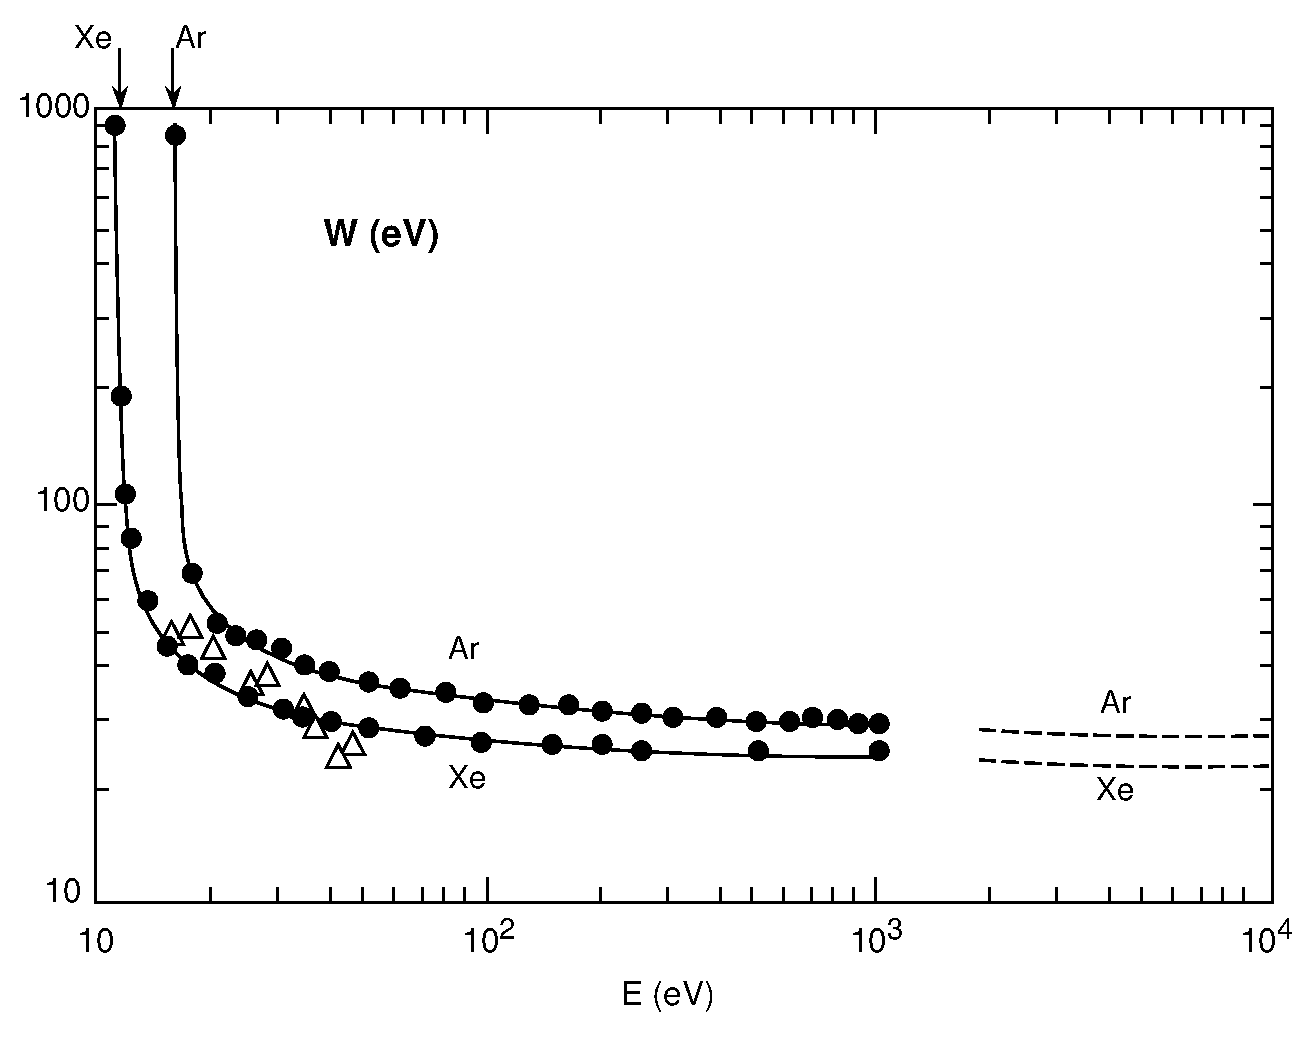
\includegraphics[width=.55\textwidth]{./pics/W.eps}
\caption{The average energy $W$ spent (in eV) for the creation
  of one electron-ion pair in Ar and Xe as a function of the incident
  energy of the ionizing particle (in this case, an electron).
  Dashed lines are extrapolations to higher energies.}
\label{fig:W}
\end{center}
\end{figure}
%%%%%%%%%%%%%%%%%%%%%%%%%%%%%%%%%%%%%%%%%%%%%%%%%%%%%%%%%%%%%%%%%%%%%%

The total number of electrons produced per interaction is
then given as the sum of the primaries and secondaries.
Thus calculating the number of electrons generated in a specific
length convolutes two distributions---a Poissonian which determines
the number of interactions, and an E$^{-n}$ which determines
the majority of the yield.  This procedure results in 
a Landau-like distribution---which is expected for the yield of 
ionization in a given path length.  Results for Ar and Ne are
shown in figure~\ref{fig:landauGases}.
%%%%%%%%%%%%%%%%%%%%%%%%%%%%%%%%%%%%%%%%%%%%%%%%%%%%%%%%%%%%%%%%%%%%%%
\begin{figure}[htb]
\begin{center}
\includegraphics[bbllx=33pt,bblly=150pt,bburx=569pt,bbury=698pt,width=.45\textwidth]{./pics/landauNe.ps}
\includegraphics[bbllx=33pt,bblly=150pt,bburx=569pt,bbury=698pt,width=.45\textwidth]{./pics/landauAr.ps}
\caption{Ionization statistics for primary, secondary, and total yield
  distributions for Ne (left panel) and Ar (right panel).  All yields
  are from a path length of 1.95~cm which is the pad length in the
  outer part of the TPC super-sector.}
\label{fig:landauGases}
\end{center}
\end{figure}
%%%%%%%%%%%%%%%%%%%%%%%%%%%%%%%%%%%%%%%%%%%%%%%%%%%%%%%%%%%%%%%%%%%%%%
Once the ionization is generated, or distributed into smaller
segments, it may then be transported to the multi-wire proportional
chamber (MWPC).

\subsection{Charge Transporter}

The charge, or ionization, in the segments that have been produced
must be transported to the sense (anode) wires of the MWPC for read-out.  
This transport is modeled in the {\bf Charge Transporter} component of 
\name{TRS}, and three distinct processes are described:
\begin{itemize}
   \item E $\times$ B Effect.
   \item Transverse and Longitudinal Diffusion.
   \item Charge Loss {\em through}
   \begin{itemize}   
     \item Absorption through attachment (O$_{2}$).
     \item Gating Grid Transparency.
     \end{itemize}
\end{itemize}
and it is possible to control each process independently.
The charge transporter calculates the position of the charge
segment/electron at the z-plane of the anode/sense wire grid
and the amount of charge that arrives.  This charge must then
be collected and amplified on the anode wires.  In the
current implementation (i.e.~{\em FAST}) the charge is simply projected
in the z coordinate to the position of the anode/sense wire plane;
the underlying assumption that the ionization follows the $\vec{E}$
field lines and no distortions are visible.  This will be refined
in future versions.

\subsubsection{E $\times$ B Effect} {\em NOTE: not currently implemented!}
        
A misalignment between the electric and magnetic fields
or inhomogeneities in the magnetic field can
give rise to the ionization following trajectories which are not 
parallel to the $\vec{E}$ field lines.  This introduces distortions
into the trajectories of ionization left in the chamber.  These are
collectively known $\vec{E} \times \vec{B}$ distortions.
In the general case of a charged particle in the presence of an 
electric and magnetic field, it will not follow a trajectory
which is described by the Langevin equation:
%%%%%%%%%%%%%%%%%%%%%%%%%%%%%%%%%%%%%%%%%%%%%%%%%%%%%%%%%%%%%%%%%%%%
\begin{equation}
\frac{d{\bf v}}{dt} = \frac{q}{m}({\bf E} + {\bf v} \times {\bf B}) - \frac{1}{\tau} {\bf v}
\label{eq:lang}
\end{equation}
%%%%%%%%%%%%%%%%%%%%%%%%%%%%%%%%%%%%%%%%%%%%%%%%%%%%%%%%%%%%%%%%%%%%
where $q$ is the charge of the particle, $m$ is its mass, {\bf v} is 
its velocity, {\bf E} the electric (drift) field, {\bf B} the 
magnetic field, and $\tau$ is the average time between collisions 
with the molecules in the medium.  The last term is essentially 
a frictional force that limits the maximum average drift velocity.  
The steady state solution (i.e.~$\frac{d{\bf v}}{dt} = 0$) is given by:
%%%%%%%%%%%%%%%%%%%%%%%%%%%%%%%%%%%%%%%%%%%%%%%%%%%%%%%%%%%%%%%%%%%%
\begin{equation}
{\bf v} = \frac{\mu |{\bf E}| }{1 + \omega ^{2} \tau ^{2}} ( \hat{\bf E} + \omega  \tau   (\hat{\bf E} \times \hat{\bf B})  + \omega ^{2} \tau ^{2}(\hat{\bf E} \cdot \hat{\bf B} )\hat{\bf B})
\label{eq:exb}
\end{equation}
%%%%%%%%%%%%%%%%%%%%%%%%%%%%%%%%%%%%%%%%%%%%%%%%%%%%%%%%%%%%%%%%%%%%
where $\mu$ $($ $= \frac{e \tau}{m})$ is the electron mobility 
and $\omega$ $($ $= \frac{e B}{m})$ is the cyclotron frequency.  
Although in the ideal field cage structure of a TPC, the electric and
magnetic fields are parallel and the drift direction is defined
by the electric field vector.  Deviations from this idealization
introduces velocity components in the orthogonal directions.

Equation~\ref{eq:exb} allows the drift velocity to be calculated at any
arbitrary spatial point given knowledge regarding the electro-magnetic
field vectors and the mobility of electrons in the gas.
The distortions can then be modeled either by numerically
integrating the equation over the drift time of the ionization, or
parameterizing the displacement of the ionization in the plane
orthogonal to the $\vec{E}$ field.

\subsubsection{Diffusion}

The effects of diffusion are due to thermal motion of the molecules
in the gas and multiple scattering of
the ionization in the transport from the position of deposition
in the chamber to the read-out or sense wires on the pad plane.
While the mean position of a charge segment may be transported through
a volume with arbitrary electro-magnetic fields according to
equation~\ref{eq:exb}, its profile will broaden
in proportion to the drift length, or more appropriately,
the square root of its drift length.
It is possible to parameterize the evolution of the size of the
charge distribution (its width) in terms of a diffusion coefficient,
which is in principle,
different in the transverse ($\sigma_{T}$) and longitudinal ($\sigma_{L}$)
directions.  This distinction is important because the evolution
of the diffusion coefficient in the transverse direction also
depends on the presence of an magnetic field where it is
reduced according to:
%%%%%%%%%%%%%%%%%%%%%%%%%%%%%%%%%%%%%%%%%%%%%%%%%%%%%%%%%%%%%%%%%%%%
\begin{equation}
{\bf \sigma_{T}(B)} = \frac{\sigma_{T}}{1 + \omega ^{2} \tau ^{2}}
\label{eq:diffusion}
\end{equation}
%%%%%%%%%%%%%%%%%%%%%%%%%%%%%%%%%%%%%%%%%%%%%%%%%%%%%%%%%%%%%%%%%%%%
Once the charge segment/cloud is transported to the read-out plane,
each segment (or sub-component) can be distributed according to a
Gaussian (or any other) distribution characterized by a width derived
from the diffusion constants.  Increasing the granularity of the
charge distribution will better reproduce single electron statistical
fluctuations.

\subsubsection{Charge Absorption}
        
The absorption of charge is a complex process that
can be attributed to many different mechanisms.\footnote{Details
  contained in a soon to be added appendix.}
For our application we consider a simple parameterization of charge
attachment in a gas where trace amounts of oxygen are present.  The
probability (P) for attachment to occur in a specified drift time, t,
is given by:        
%%%%%%%%%%%%%%%%%%%%%%%%%%%%%%%%%%%%%%%%%%%%%%%%%%%%%%%%%%%%%%%%%%%%
\begin{equation}
             P(t) = 1 - e^{-At}
\label{eq:attach}
\end{equation}
%%%%%%%%%%%%%%%%%%%%%%%%%%%%%%%%%%%%%%%%%%%%%%%%%%%%%%%%%%%%%%%%%%%%
where A specifies an {\em attachment rate} given by:
%%%%%%%%%%%%%%%%%%%%%%%%%%%%%%%%%%%%%%%%%%%%%%%%%%%%%%%%%%%%%%%%%%%%
\begin{equation}
            A = P_{O_{2}} \cdot P_{M} \cdot C_{O_{2},M}
\label{eq:attachrate}
\end{equation}
%%%%%%%%%%%%%%%%%%%%%%%%%%%%%%%%%%%%%%%%%%%%%%%%%%%%%%%%%%%%%%%%%%%%
where P$_{O2}$ and P$_{M}$ are the partial
pressures of the oxygen and TPC gas respectively.
C$_{O2,M}$ specifies an {\em attachment coefficient} which
is a function of the gas in question and the reduced electric field (E/p).
For the case of STAR, a value of C = 10.2~$\mu$s$^{-1}$~bar$^{-2}$
has been deduced.\footnote{soon to be added appendix.}
To give an idea of the order of magnitude, for a concentration
of oxygen of 50~ppm and an ionization cloud drifting for
50~$\mu$s, the charge loss is expected to be approximately 2.5\%.
This charge loss can be applied at the single electron level or
an extended charge cloud where a fraction of the total is lost.

\subsubsection{Wire Grid Transparency}
        
As the charge enters the region of the wire grids in the
TPC, there is a non-zero probability that the charge may not
be transmitted due to the potential configuration on the wire
grids.  In the STAR TPC there are three wire grids:
%%%%%%%%%%%%%%%%%%%%%%%%%%%%%%%%%%%%%%%%%%%%%%%%%%%%%%%%%%%%%%%%%%%%
\begin{itemize}
   \item anode/sense---responsible for charge collection and
     amplification.
   \item zero/frisch---defines the boundary of the field cage and
     allows a sink for ion collection in the amplification process.
   \item gate---switch which controls passage of ionization from
     the active TPC volume to the sense/anode wire plane.
\end{itemize}
%%%%%%%%%%%%%%%%%%%%%%%%%%%%%%%%%%%%%%%%%%%%%%%%%%%%%%%%%%%%%%%%%%%%
The passage of ionization is controlled by the potential which
is applied to the gate wires.  Basically by setting the appropriate
potential on this grid, the drift $\vec{E}$ lines can be made to
terminate on the gating grid (zero transparency) or at the anode
wires (full transparency).  The transparency is the fraction of
lines that terminate on the anode wires compared to those that
terminate on the gating grid.

A general expression for the transparency of a mono-stable switched
gating grid was deduced such that
the full range from 0-100\% transmission can be
modeled.  It should be noted that the effects of a bi-polar switching
grid (which is the actual construction of the STAR-TPC) should not
influence the values at more than the $\sim$5\% level.
The expressions involved require only the geometry of the
wire grids and the voltages set on the gating grid
and high-voltage plane.  An example of the transmission curve
is shown in figure~\ref{fig:gridTransparency}.
%%%%%%%%%%%%%%%%%%%%%%%%%%%%%%%%%%%%%%%%%%%%%%%%%%%%%%%%%%%%%%%%%%%%
\begin{figure}[htb]
\begin{center}
\includegraphics[bbllx=14pt,bblly=137pt,bburx=569pt,bbury=701pt,width=.55\textwidth]{./pics/gridTransparency.ps}
\caption{Wire Grid Transparency Calculation for nominal wire potentials
  and STAR outer sector read-out chamber geometry.}
\label{fig:gridTransparency}
\end{center}
\end{figure}
%%%%%%%%%%%%%%%%%%%%%%%%%%%%%%%%%%%%%%%%%%%%%%%%%%%%%%%%%%%%%%%%%%%%%%

\subsection{Charge Collection}

According to the position of the charge segment/electron at the
anode wire plane, the ionization can be collected by the nearest wire.
The appropriate time delays for charge collection should a segment not
be projected directly on top of the wire position can be calculated.
Once the charge is assigned to a wire, the gas amplification can occur.

\subsubsection{Gas Gain Amplification at Sense Wires}

The process of gas amplification at the sense wires is modeled
by the Raether distribution,\footnote{see http://www.rhic.bnl.gov/STAR/html/comp\_l/simu/TpcRespSim/src/literature.html}
or, as it is denoted in Blum and Rolandi\footnote{W.~Blum and L.~Rolandi
  {\em Particle Detection with Drift Chambers} Springer-Verlag 1994.},
the Yule-Furry process which
describes the fluctuations in the amplification an amount of
charge q with an exponential distribution:
%%%%%%%%%%%%%%%%%%%%%%%%%%%%%%%%%%%%%%%%%%%%%%%%%%%%%%%%%%%%%%%%%%%%%%
\begin{equation}
          p(q) = \frac{1}{\bar{q}} e^{-q/\bar{q}}
\label{eq:raether}
\end{equation}
%%%%%%%%%%%%%%%%%%%%%%%%%%%%%%%%%%%%%%%%%%%%%%%%%%%%%%%%%%%%%%%%%%%%%%
Subsequent theoretical refinements to this simple expression which
were made in order to take into account effects like
the asymmetric growth of the avalanche profile as well as saturation
effects.  This resulted in several distribution, the Polya distribution
being the most popular.  It requires an additional parameter to supplement
the mean amplification ($\bar{q}$).  The effect of the additional parameter
is to suppress the small amplification factors.
As this parameter tends to zero, the Raether distribution is recovered.
Experimentally, perfectly exponential behavior is seen at
low to moderate gas gains (i.e.$<$10$^{4}$), in parallel plate geometry,
however at gas gains above 10$^{5}$, slight deformation from
exponential shape is observed.  This is probably
attributable to self-saturation effects which
become important because of space charge.  Since the TPC is generally
operated at low gas gains, the simple Raether distribution was
deemed acceptable, however the Polya function may be substituted
if there is need.

It should be noted that in TPC (or any drift chamber) operation,
the effect of the fluctuations in gas gain is to simply degrade the
attainable space-point resolution, and for this purpose the exact
functional form of the avalanche yields is not absolutely critical.
This degradation is the physics that the implementation of the gas-gain
fluctuations will attempt to address, and the Raether distribution should
be quite acceptable in this regard.

Once the charge has been amplified, the amount of charge induced on
the cathode pad plane can then be calculated.

\subsection{Analog Signal Generation}

The Analog Signal Generator has three main functions:
%%%%%%%%%%%%%%%%%%%%%%%%%%%%%%%%%%%%%%%%%%%%%%%%%%%%%%%%%%%%%%%%%%
\begin{itemize}
   \item Determine the charge induced on single pads from the charge
     ``collected'' on the anode wires.
   \item Sample the induced charge signals in time according to the
     electronics (i.e~pre-amplifier/shaper) response.
   \item Distribute the \underline{\bf analog} charge into time bins
     according to the parameters of the switched capacitor array (SCA).
   \end{itemize}
%%%%%%%%%%%%%%%%%%%%%%%%%%%%%%%%%%%%%%%%%%%%%%%%%%%%%%%%%%%%%%%%%%

\subsubsection{Charge Induction}

The charge induced on a grounded pad plane by a point charge $q$ located
a distance $d$ above the plane can be calculated by the method of
images.  The charge density ($\sigma$) on the plane is given by:
%%%%%%%%%%%%%%%%%%%%%%%%%%%%%%%%%%%%%%%%%%%%%%%%%%%%%%%%%%%%%%%%%%
\begin{equation}
  \sigma (x,y) = \frac{1}{2 \pi} \frac{q d}{((x-x_{o})^{2} + (y-y_{o})^{2} + d^{2})^{3/2}}
\label{eq:imageQ}
\end{equation}
%%%%%%%%%%%%%%%%%%%%%%%%%%%%%%%%%%%%%%%%%%%%%%%%%%%%%%%%%%%%%%%%%%
where the charge $q$ is located at a position (x$_{o}$,y$_{o}$).  However
this expression is not the solution for the charge induced on the pad
plane of a wire chamber.  In the case of a MWPC the charge, which
is at the position of the anode wire, is generally surrounded by {\em two}
cathode planes---one from
above and one from below.\footnote{Also the charge is in the form of
  a line charge associated with a linear charge density, not a
  discrete point charge.}
Thus in order to calculate the charge density induced on the pad
plane, all higher order multi-pole terms must be incorporated.
This results in the following expression:
%%%%%%%%%%%%%%%%%%%%%%%%%%%%%%%%%%%%%%%%%%%%%%%%%%%%%%%%%%%%%%%%%%
\begin{equation}
\sigma (x,y) = \frac{1}{2 \pi} \sum_{n}^{\infty} \frac{(2n+1) q d}{((x-x_{o})^{2} + (y-y_{o})^{2} + ((2n+1) d)^{2})^{3/2}}
\label{eq:imageQ2}
\end{equation}
%%%%%%%%%%%%%%%%%%%%%%%%%%%%%%%%%%%%%%%%%%%%%%%%%%%%%%%%%%%%%%%%%%
Doing the sum, (and integrating over all y) yields a function
which describes the charge distribution induced on the
pad plane at a distance $x$ from the wire where $x_{o}$ is
the position of the charge $q$:
%%%%%%%%%%%%%%%%%%%%%%%%%%%%%%%%%%%%%%%%%%%%%%%%%%%%%%%%%%%%%%%%%%
\begin{equation}
\sigma(x,y) = \frac{q}{4 d \cosh(\frac{\pi (x- x_{o})}{2 d})}
\label{eq:endo1}
\end{equation}
%%%%%%%%%%%%%%%%%%%%%%%%%%%%%%%%%%%%%%%%%%%%%%%%%%%%%%%%%%%%%%%%%%
This function, an inverse hyperbolic cosine as shown in
equation~\ref{eq:endo1} is called an {\em Endo function}.  Note that the
derivation put no limits on the extent of the pad in the y direction
(i.e.~$\frac{w}{l}=0$).
The effect of finite geometry of segmented cathodes can be accounted
for with the addition of another parameter.  The same function can
be written in a form more instructive for our purposes:
%%%%%%%%%%%%%%%%%%%%%%%%%%%%%%%%%%%%%%%%%%%%%%%%%%%%%%%%%%%%%%%%%%
\begin{equation}
\sigma(x) = K_{1} \frac{1 - \tanh^{2}(\frac{\pi (x-x_{o})}{4 d})}{1 + \tanh^{2}(\frac{\pi (x-x_{o})}{4 d})}
\label{eq:endo2}
\end{equation}
%%%%%%%%%%%%%%%%%%%%%%%%%%%%%%%%%%%%%%%%%%%%%%%%%%%%%%%%%%%%%%%%%%
where K$_{1}$ is a normalization constant.  Equation~\ref{eq:endo2}
can be used to generalize the Endo function in order to account for
finite geometry effects of the segmented cathode pads.  That is, each
pad has a finite width/length ratio.  This can be accounted for with
the addition of another constant K$_{2}$:
%%%%%%%%%%%%%%%%%%%%%%%%%%%%%%%%%%%%%%%%%%%%%%%%%%%%%%%%%%%%%%%%%%
\begin{equation}
  F(x) = K_{1} \frac{1 - \tanh^{2}(\frac{\pi (x-x_{o})}{4 d})}{1 + K_{2} \tanh^{2}(\frac{\pi (x-x_{o})}{4 d})}
\label{eq:gatti}
\end{equation}
%%%%%%%%%%%%%%%%%%%%%%%%%%%%%%%%%%%%%%%%%%%%%%%%%%%%%%%%%%%%%%%%%%
This is the generalized solution to the distribution of
charge induced on a grounded pad plane by a point/line charge,
and is usually dubbed, the Gatti function.  The Gatti function
is most prevalently used for pad chamber responses.  Although
more accurate, the price that is paid is the increase in time
required to integrate equation~\ref{eq:gatti} over the rather
simple expression which can be deduced from the integral of~\ref{eq:endo1}
A comparison of the Gatti and Endo functions to a Gaussian
(for reference) are given in figure~\ref{fig:gatti}
%%%%%%%%%%%%%%%%%%%%%%%%%%%%%%%%%%%%%%%%%%%%%%%%%%%%%%%%%%%%%%%%%%%%
\begin{figure}[htb]
\begin{center}
\includegraphics[bbllx=18pt,bblly=146pt,bburx=563pt,bbury=691pt,width=.55\textwidth]{./pics/prfShape.ps}
\caption{Comparison of Gaussian, Endo, and Gatti functions for profiles
  of the pad-response-function.}
\label{fig:gatti}
\end{center}
\end{figure}
%%%%%%%%%%%%%%%%%%%%%%%%%%%%%%%%%%%%%%%%%%%%%%%%%%%%%%%%%%%%%%%%%%%%%%

For the case of the TPC, the quantity of interest is the total
amount of charge ($Q$) induced per pad which means one must integrate
these functions, which specify the charge density, according to the
pad dimensions.  Thus for a point charge (equation~\ref{eq:imageQ}),
the integral is:
%%%%%%%%%%%%%%%%%%%%%%%%%%%%%%%%%%%%%%%%%%%%%%%%%%%%%%%%%%%%%%%%%%
\begin{equation}
  Q = \frac{1}{2 \pi} \int_{yl}^{yu} \int_{xl}^{xu} dx dy \frac{q d}{((x-x_{o})^{2} + (y-y_{o})^{2} + d^{2})^{3/2}}
  \label{eq:imageQint}
\end{equation}    
%%%%%%%%%%%%%%%%%%%%%%%%%%%%%%%%%%%%%%%%%%%%%%%%%%%%%%%%%%%%%%%%%%
where $xl$ and $xu$ denotes the lower and upper bounds of
the pad in the x direction respectively.  Similarly $yl$ and $yu$
denotes the same in the y
direction.  Similar integrals can be constructed given any
arbitrary charge density ($\sigma$).  The advantage of using such functions
is that they allow the production of longer tails which have
non-Gaussian characteristics.  The tails are an important characteristic
to understand as they determine the efficiency of the ionization
collection which is very important in the
study of ionization collection for $\frac{dE}{dx}$ resolution.
Furthermore these integrals are well defined
given the the position of the charge and the coordinates
of the pads.  Thus charge induced on adjacent pads as well as rows
can be also be calculated quite simply in this formalism.
Illustrations of some of these
function are shown in figures~\ref{fig:gatti}.\footnote{For more
  details see: http://www.rhic.bnl.gov/STAR/html/comp\_l/simu/TpcRespSim/src/literature.html} 

%%%%%%%%%%%%%%%%%%%%%%%%%%%%%%%%%%%%%%%%%%%%%%%%%%%%%%%%%%%%%%%%%%%%
%\begin{figure}[htb]
%\begin{center}
%\includegraphics[bbllx=14pt,bblly=137pt,bburx=569pt,bbury=701pt,width=.55\textwidth]{}
%\caption{Comparison of Gaussian, Endo, and Gatti functions for PRF.}
%\label{fig:xxx}
%\end{center}
%\end{figure}
%%%%%%%%%%%%%%%%%%%%%%%%%%%%%%%%%%%%%%%%%%%%%%%%%%%%%%%%%%%%%%%%%%%%%%
Please keep in mind that the fact that the signal on the wire is
due almost exclusively to the motion of the charged ions {\bf away} from
the wire.  In order to calculate the total amount of charge induced
on the pad however, it is possible to use the number of electrons
as a quantity, even though they are not the physical reason for
the charge induction.  This point will be reiterated in the electronics
response of this description.

\subsubsection{Sample the Signal in Time}

Once the amount and centroid of the charge distribution
on each pad is determined, this charge can be sampled in
time corresponding to the analog electronics response.
The signals are generated by super-imposing each analog signal
from each avalanche which induces a signal on the pad plane.
This allows the shaping
time of the electronics can be varied independently of
the width of the pad response function which is the strength
of this simulation methodology.  Currently four types of
sampling are possible:
%%%%%%%%%%%%%%%%%%%%%%%%%%%%%%%%%%%%%%%%%%%%%%%%%%%%%%%%%%%%%%%%%%
\begin{itemize}
  \item delta function.
  \item Symmetric Gaussian.
  \item Asymmetric Gaussian.
  \item Parameterized STAR response.
\end{itemize}
%%%%%%%%%%%%%%%%%%%%%%%%%%%%%%%%%%%%%%%%%%%%%%%%%%%%%%%%%%%%%%%%%%
A function also exists where a fractional scale of the total charge integral
can be added as an Undershoot/Unrestored baseline component in the
signal which has the effect of convoluting effects from the long 1/T tail.
This is an important point and one that actually blurs the line of
physics and simulation.  In reality the
time evolution of the signal that is developed on the wires is nearly 
entirely due to the {\bf motion of the positive ions} away from the wire.
This produces a signal with a long 1/T tail.  For the STAR geometry
the signal is $\sim$62~$\mu$s.  In order to make a detector faster,
the signal is differentiated after a characteristic time---the
shaping time of the pre-amplifier.  Although the detector response
becomes faster, the trade-off is that only a fraction of the total
charge is seen by the downstream electronics (i.e.~the ADC).  This
fraction $F$, is given by:
%%%%%%%%%%%%%%%%%%%%%%%%%%%%%%%%%%%%%%%%%%%%%%%%%%%%%%%%%%%%%%%%%%
\begin{equation}
  F = \frac{ln(1+\frac{t_{m}}{t_{o}})}{ln(1+\frac{t_{s}}{t_{o}})}
  \label{eq:fraction}
\end{equation}    
%%%%%%%%%%%%%%%%%%%%%%%%%%%%%%%%%%%%%%%%%%%%%%%%%%%%%%%%%%%%%%%%%%
where t$_{m}$ is the length of time the undifferentiated signal would
persist (i.e.~$\sim$62~$\mu$s), t$_{o}$ is the characteristic time
of the signal development (i.e.~$\sim$1~ns), and t$_{s}$ is the shaping
time of the pre-amplifier (i.e.~$\sim$180~ns).  For STAR this implies
the order of 45\% of the charge is distributed into time bins by the
SCA.  More importantly is that the signal shape is dominated very strongly
by the shaping properties of the electronics.  Thus the
long time response of the chamber is parameterized in the electronics
processing component of the simulator, rather than modeling the
motion of the positive ions.

The symmetric Gaussian response, with the effect of an unrestored baseline
due to under/over shoot is illustrated in figure~\ref{fig:baseline}
%%%%%%%%%%%%%%%%%%%%%%%%%%%%%%%%%%%%%%%%%%%%%%%%%%%%%%%%%%%%%%%%%%%%
\begin{figure}[htb]
\begin{center}
\includegraphics[bbllx=14pt,bblly=137pt,bburx=569pt,bbury=701pt,width=.55\textwidth]{./pics/baseline.ps}
\caption{Asymmetric Gaussian Electronics Response with pedestal suppressed
  showing both undershoot (top panel) and an under damped
  baseline restoration (bottom panel).}
\label{fig:baseline}
\end{center}
\end{figure}
%%%%%%%%%%%%%%%%%%%%%%%%%%%%%%%%%%%%%%%%%%%%%%%%%%%%%%%%%%%%%%%%%%%%%%
where the time evolution of a series of 20 signals, of identical
amplitude, are induced on a single pad.\footnote{More examples can
  be seen at: http://www.rhic.bnl.gov/STAR/html/comp\_l/simu/TpcRespSim/src/literature.html} 
The pulses are simply added using the principle of super-position.
The modeling of an unrestored baseline is very
important since the pulse height (actually the integral) of the
signal is used as a measure of the velocity of the particle
(via $\frac{dE}{dx}$ information).
An unrestored baseline due to undershoot can result in
an effective loss of charge in a high-multiplicity environment.  Conversely
an unrestored baseline due to under-damping will result in too much
charge being observed at large drift distances.  Both effects
will reduce the attainable resolution if not taken into account.  

Once the complete functional form of the signals induced on a pad
over the read-out period of the TPC electronics, the analog charge
can be distributed into discrete time bins. This sampling simulates
the behavior of the switched capacitor array (SCA) in the front-end
electronics.  This is done by integrating the amount of charge in
a time interval $\Delta$t, which is determined from the SCA sampling
frequency.  Chamber noise as well as electronic noise
can be added at this point.

\subsection{Digital Signal Generation}

Once the analog charge is distributed into time bins on the pads,
the digitization can occur.  This is currently a simple
conversion from voltage to ADC counts.  Other features
such as the addition of a pedestal
and non-linearities in the ADC can also be added.
In fact, any characteristic of the
digital electronics can be added and will be independent
of the analog signal sampling.  This is very close to
the way the front-end electronics are designed where the
digital and analog electronic components are separated.

\section{Physics Limitations}

There are still some components either not implemented,
or completely missing from TRS in its current form.  It
is hoped that these will be incorporated as the understanding
of TRS evolves.  Most critically is the noise.  Although some
preliminary work exists for this modeling, it has currently not
reached a mature enough state where it can be added.  Some obvious
short-comings are listed below.
%%%%%%%%%%%%%%%%%%%%%%%%%%%%%%%%%%%%%%%%%%%%%%%%%%%%%%%%%%%%%%%%%%%%
\begin{itemize}
  \item $\vec{E} \times \vec{B}$ in not tested although code exists
    and can be "plugged" in.
  \item Noise at the chamber and electronics level does not yet exist.
  \item A function (or look-up table) is needed for the non-linear ADC
    response.
  \item The pad geometry is not incorporating the fractional pads at the
    border of the sectors.
  \item The gas gain is currently independent of the wire and the
    position of the avalanche on the wire.
  \item Effects of space charge in the charge transport stage of the
    simulation.
  \item No positional dependence in the transparency of the gating grid
    exists.  Currently a constant transparency, independent of position
    is calculated.
\end{itemize}
%%%%%%%%%%%%%%%%%%%%%%%%%%%%%%%%%%%%%%%%%%%%%%%%%%%%%%%%%%%%%%%%%%%%

It is almost certain that as
experience is gained with the package, this list will be further
expanded, however the code is written in a flexible manner such that
these type of additions should be relatively straight forward.

\section{Known Limitations} \index{limitations}

To be seen... 

\section{Support and Reporting Bugs} \index{support}

Currently \name{TRS} is supported by a small group.  Hopefully
as more people begin to use it and add to it, there will be a larger
support base for it.  If there is a problem or bug, report it to
one or more of the following:
\begin{itemize}
  \item starsas-l@bnl.gov
  \item starsofi-l@bnl.gov
  \item startpc-l@bnl.gov
  \item brian.lasiuk@yale.edu
  \item thomas.ullrich@yale.edu
\end{itemize}

\clearpage

%%%%%%%%%%%%%%%%%%%%%%%%%%%%%%%%%%%%%%%%%%%%%%%%%%%%%%%%%%%%%%%%%%%%
%
%    Reference Manual
%
%%%%%%%%%%%%%%%%%%%%%%%%%%%%%%%%%%%%%%%%%%%%%%%%%%%%%%%%%%%%%%%%%%%%
\part{Reference Manual}
\clearpage

This reference manual is broken into six sections.  The first 
section describe the {\em Data Base interfaces and implementations} 
within \name{TRS}.  The second describes the {\em Coordinate systems} and the
{\em Coordinate transformation functor}.  The next two sections describe
the {\em Containers} and {\em Physics Processes} that are accessible and
utilized in \name{TRS}.  The fifth section is not yet complete but
will include the {\em Administrative} type
classes that are utilized while the final section contains
an {\em Example} and describes how
the package is used in an example program.  Within the categories,
as much as possible, the listing of classes are alphabetical, and
closely related classes which either inherit or are derived are
cross-referenced.  

As mentioned previously, heavy use of the SCL \index{SCL} is made
within \name{TRS}, so that manual is also a useful reference.  It
can be found at: http://star.physics.yale.edu/SCL.  As such, many
conventions adopted in the SCL are carried through into \name{TRS}
in order to ensure compatibility.  As {\bf namespaces} are not
currently supported
widely among vendor or commercial compilers, the current STAR
conventions advocate the addition of prefixes to indicate the
scope of a class.  {\bf St}
denotes all STAR specific classes.  This prefix is supplemented with
{\bf Trs} to denote \name{TRS} specific classes where appropriate.  As an
extension, the prefix {\bf Tpc} is also used occasionally.

%%%%%%%%%%%%%%%%%%%%%%%%%%%%%%%%%%%%%%%%%%%%%%%%%%%%%%%%%%%%%%%%%%%%%%%%
%@@@                                                                   %
%                       DataBase and Interfaces                        %
%                                                                      %
%%%%%%%%%%%%%%%%%%%%%%%%%%%%%%%%%%%%%%%%%%%%%%%%%%%%%%%%%%%%%%%%%%%%%%%%

\section{Data Base and Interfaces}
\label{sec:dbint}
Following are descriptions of the four different data base interfaces
and implementations.

%%%%%%%%%%%%%%%%%%%%%%%%%%%%%%%%%%%%%%%%%%%%%%%%%%%%%%%%%%%%%%%%%%%%
%
%    Reference: StMagneticField
%
%%%%%%%%%%%%%%%%%%%%%%%%%%%%%%%%%%%%%%%%%%%%%%%%%%%%%%%%%%%%%%%%%%%%
\subsection{StMagneticField} \index{StMagneticField}
\label{sec:stMagneticField}
\begin{Entry}
\item[Summary]
  Interface which defines access methods to the magnetic field components.

\item[Synopsis]
  Purely abstract class, no instantiation is  possible.
  
\item[Description]
Class StMagneticField is an abstract class that defines
the interface that is used to access the magnetic field components.

\item[Persistence]
   None

\item[Related Classes]
The implementation of the magnetic field data base is done in
the class {\bf StSimpleMagneticField}.  
See section~\ref{sec:stSimpleMagneticField}.

\item[Dependencies]
Requires \comp{StGlobalCoordinate} \index{StGlobalCoordinate}
from \name{TRS}\comp{StThreeVector} from the SCL \index{StThreeVector}.

\item[Public \\ Constructors]
   None

\item[Public \\ Virtual Operators]
   None

\item[Public Virtual \\ Member Functions]

  \verb+virtual const StThreeVector<double>&+\\
  \verb+at(const StGlobalCoordinate& gp)+\\
  Provides access to the magnetic field components in an StThreeVector
  at a position, gp specified in the STAR global coordinate system.

\end{Entry}
\clearpage

%%%%%%%%%%%%%%%%%%%%%%%%%%%%%%%%%%%%%%%%%%%%%%%%%%%%%%%%%%%%%%%%%%%%
%
%    Reference: StSimpleMagneticField
%
%%%%%%%%%%%%%%%%%%%%%%%%%%%%%%%%%%%%%%%%%%%%%%%%%%%%%%%%%%%%%%%%%%%%
\subsection{StSimpleMagneticField} \index{StSimpleMagneticField}
\label{sec:stSimpleMagneticField}
\begin{Entry}
\item[Summary]
  Implementation of a simple data base which provides the magnetic 
  field components which are read from an ASCII file.

\item[Synopsis]
  \verb+#include "StSimpleMagneticField.hh"+\\
  requires \comp{StGlobalCoordinates.hh} from \name{TRS}. 
  \comp{StThreeVector.hh} as well as \comp{StGetConfigValue}
  are required from the SCL. \index{SCL}   The \comp{SystemOfUnits} class in 
  the SCL is also used to ensure a uniform usage of the unit types.
  
\item[Description]
Class StSimpleMagneticField is a concrete class that implements
methods defined by the abstract base class \comp{StMagneticField}
(see section~\ref{sec:stMagneticField}).  Values
of the field are accessed given a global coordinate (\comp{StGlobalCoordinate})
as described in section~\ref{sec:stGlobalCoordinate}.  The field
value is returned as a \comp{StThreeVector} which is currently
of double precision.
The implementation of the "simple" data base uses the \comp{StGetConfigValue}
utility from the SCL which parses an ASCII file which reads the
numerical value of the magnetic field specified by a key word.  The
field values are kept as data members, and the access functions
simply return the value.  This initialization is done in the {\em private}
constructor(s).  Currently a constant field 
with the field components specified as (B$_{x}$,B$_{y}$,B$_{z}$) 
given as (0,0,.5)~Tesla, at any coordinate, is implemented.
The data base is implemented as a singleton class \index{singleton}
which protects the code against multiple distinct copies of the
data base parameters in the code.  As such the class constructors
are implemented as {\em private} data members which are called
via a {\em public} member function:

\item[Persistence]
   None

\item[Related Classes]
The base class which defines the interface is specified in
the class \comp{StMagneticField}.  
See section~\ref{sec:stMagneticField}.

\item[Public \\ Constructors]

   \verb+static StMagneticField* instance(const char* file)+\\
   Returns a pointer of type \comp{StMagneticField}.  The {\em static}
   designation implies at most, one instance of this can occur.
   The pointer will be returned if and only if a file name (file) 
   suitable to initialize the class is specified.  Such a file
   is provided in TRS in the {\bf run} directory (run/example.conf).
   Subsequent 
   declarations of magnetic fields can be made in the code, but
   once the first instance is created, the same pointer will
   be returned.

   \verb+static StMagneticField*+\\
   \verb+instance(const StThreeVector<double>& B)+\\
   Returns a pointer of type \comp{StMagneticField}.  The {\em static}
   designation implies at most, one instance of this can occur.
   The pointer will be returned if and only if an StThreeVector, B
   is supplied which will specify the field components at
   every spatial location.  This is useful if a constant field
   is required.  Subsequent 
   declarations of magnetic fields can be made in the code, but
   once the first instance is created, the same pointer will
   be returned.
   
   \verb+static StMagneticField* instance()+\\
   Returns the pointer of type StMagneticField should an instance
   of the class have been made previously, otherwise a filename
   or three-vector need be specified for the first initialization.

\item[Private \\ Constructor]

   The constructors are hidden from direct call to ensure that
   only one instance of the data base is made.  As such, the
   constructors are only called through member functions
   as described above.  The {\em actual} constructors which are
   called are:

   \verb+StSimpleMagneticField(const char* file)+\\
   Called from the member function \texttt{instance(const char* file)}
   which is only invoked if a previous instance is not detected.
   The parsing of the ASCII file is done in this constructor to
   initialize the data members.  The file is provided in the {\bf run}
   directory of the package.

   \verb+StSimpleMagneticField(const StThreeVector<double>& B)+\\
   Called from the member function {\em instance(const StThreeVector$<$double$>$\& B)}
   if and only if
   a previous instance is not detected.  The data member which
   stores the magnetic field is initialized in this constructor.

   \verb+StSimpleMagneticField()+\\
   Never called, rather the member function \texttt{instance()}
   returns the \comp{StMagneticField} pointer which was created by 
   a previous instance.  No initialization of data members is
   done in this constructor.

\item[Public \\ Operators]
   None

\item[Public \\ Member Functions]

  Following are implementations of the functions defined in
  the interface \comp{StMagneticField}.

  \verb+const StThreeVector<double>&+\\
  \verb+         at(const StGlobalCoordinate& gp) const+\\
  Returns the magnetic field components in an \comp{StThreeVector}
  at a position, gp specified in the STAR global coordinate system.

  \verb+const StThreeVector<double>&+\\
  \verb+         at(const StThreeVector<double>& gp) const+\\
  Returns the magnetic field components in an \comp{StThreeVector}
  at a position, gp specified in the STAR global coordinate system.

\item[Examples]
{\footnotesize
\begin{verbatim}
#include <iostream.h>
#include <unistd.h>    // needed for access()
#include <string>

// SCL
#include "SystemOfUnits.h"

// TRS
#include "StCoordinates.hh"
#include "StSimpleMagneticField.hh"

int main()
{
    // Check File access

    string magFile("../run/example.conf");
    if (access(magFile.c_str(),R_OK)) {
        cerr << "ERROR:\n" << magFile << " cannot be opened" << endl;
        exit(1);
    }
    
    // Create an instance of the DataBase

    StMagneticField *magDb =
        StSimpleMagneticField::instance(scFile.c_str());

   // Print the data base to the screen
  
   magDb->print();

   // Access to the field at a spatial point

   StGlobalCoordinate 
      myCoordinate(0.*centimeter, 0.*centimeter, 0.*centimeter);
   StThreeVector<double> field = magDb->at(myCoordinate);
  
   cout << "Magnetic Field at " << myCoordinate << " is " 
        << field << " T." << endl;
    
    return 0;
}
\end{verbatim}
}%footnotesize    
{\bf Programs Output:}
{\footnotesize
\begin{verbatim}

To be run

\end{verbatim}
} %footnotesize

\end{Entry}
\clearpage


%%%%%%%%%%%%%%%%%%%%%%%%%%%%%%%%%%%%%%%%%%%%%%%%%%%%%%%%%%%%%%%%%%%%
%
%    Reference: StTpcElectronics
%
%%%%%%%%%%%%%%%%%%%%%%%%%%%%%%%%%%%%%%%%%%%%%%%%%%%%%%%%%%%%%%%%%%%%
\subsection{StTpcElectronics} \index{StTpcElectronics}
\label{sec:stTpcElectronics}
\begin{Entry}
\item[Summary]
  Interface which defines access functions to electronics specific
  constants or parameters.      

\item[Synopsis]
  Purely abstract class, no instantiation is  possible.
  
\item[Description]
Class \comp{StTpcElectronics} is an abstract base class that defines
the interface that is used to access all TPC electronics related 
parameters.  This includes both the analog and digital components of 
the TPC electronics.

\item[Persistence]
   None

\item[Related Classes]
The implementation of the electronics data base is done in
the class \comp{StTpcSimpleElectronics}.

\item[Public \\ Constructors]
   None

\item[Public \\ Virtual Operators]
   None

\item[Public Virtual \\ Member Functions]

  {\bf Analog Electronics\\} \index{Analog Electronics}
  \verb+virtual double nominalGain() const+\\
  Provides access to the nominal gain of the pre-amplifier in mV/fC.

  \verb+virtual double channelGain(int s,int r,int p) const+\\
  Provides access to the individual channel gain of the pre-amplifier
  indexed  by the sector (s), pad row (r), and pad (p).  This function
  should be more relevant once an electronics gain calibration has been
  done.

  \verb+virtual double channelGain(StTpcPadCoordinate& c) const+\\
  Provides access to the individual channel gain of the pre-amplifier  
  indexed  given a StTpcPadCoordinate (c).  
  See section~\ref{sec:rawCoordinate}.

  \verb+virtual double shapingTime() const+\\
  Provides access to the shaping time of the pre-amplifier shaper.

  \verb+virtual double samplingFrequency() const+\\
  Provides access to the sampling frequency of the switched capacitor 
  array (SCA) \index{SCA}.

  {\bf Digital Electronics \\}
  \verb+virtual double adcConversion() const+\\
  Provides access to the nominal ADC conversion value.

  \verb+virtual double adcConversionCharge() const+\\
  Provides access to the nominal ADC conversion value.

  \verb+virtual int averagePedestal() const+\\
  Provides access to the nominal pedestal value for the ADC.

  \verb+virtual int pedestal(int s,int r, int p, int t) const+\\
  Provides access to the pedestal value for a single ADC channel indexed
  by a sector (s), pad row (r), pad (p), and time bin (t).  Should
  be more relevant once a real electronics calibration has been done.

  \verb+virtual int pedestal(StTpcPadCoordinate&) const+\\
  Provides access to the pedestal value for a single ADC channel specified
  by a raw pad coordinate.  See section~ref{sec:rawCoordinate}.

  {\bf Diagnostic\\} \index{Analog Electronics}
  \verb+virtual void print(ostream& = cout) const+\\
  Prints the values of all constants accessible by public access
  functions to an output file stream.  The default is the screen.

\item[Examples]
  None

\end{Entry}
\clearpage

%%%%%%%%%%%%%%%%%%%%%%%%%%%%%%%%%%%%%%%%%%%%%%%%%%%%%%%%%%%%%%%%%%%%
%
%    Reference: StTpcGeometry
%
%%%%%%%%%%%%%%%%%%%%%%%%%%%%%%%%%%%%%%%%%%%%%%%%%%%%%%%%%%%%%%%%%%%%
\subsection{StTpcGeometry \index{StTpcGeometry|textbf}}
\label{sec:stTpcGeometry}

\begin{Entry}
\item[Summary]
    Interface which defines access functions to geometrical specific
    constants or parameters.
    
\item[Synopsis]
    Purely abstract class; instantiation is not possible.

\item[Description]  
Class \comp{StTpcGeometry} is an abstract base class that defines
the interface that is used to access all geometrical parameters 
related to the TPC including the field cage, pad-plane, and read-out
chamber.

\item[Persistence]
   None

\item[Related Classes]
The implementation of the geometry data base is done in
the class \comp{StTpcSimpleGeometry}. \index{StTpcSimpleGeometry}
  
\item[Public \\ Constructors]
   None

\item[Public \\ Virtual Operators]
   None

\item[Public Virtual \\ Member Functions]

  {\bf Rows \\}
  \verb+virtual int numberOfRows() const+\\
  Provides access to the number of rows in a single super sector.

  \verb+virtual int numberOfInnerRows() const+\\
  Provides access to the number of rows in the inner part of a super sector.

  \verb+virtual int numberOfInnerRows48() const+\\
  Provides access to the number of rows in the inner part of a super sector
  where the row pitch is 48~mm.

  \verb+virtual int numberOfInnerRows52() const+\\
  Provides access to the number of rows in the inner part of a super sector
  where the row pitch is 52~mm.

  \verb+virtual int numberOfOuterRows() const+\\
  Provides access to the number of rows in the outer part of a super sector.

  \verb+virtual double innerSectorRowPitch1() const+\\
  Provides access to the pitch of the rows in the 8 innermost pad rows
  of the inner super sector.

  \verb+virtual double innerSectorRowPitch2() const+\\
  Provides access to the pitch of the rows in the 5 outermost pad rows
  of the inner super sector.

  \verb+virtual double outerSectorRowPitch() const+\\
  Provides access to the pitch of the rows in the outer part of a super sector.
    
  \verb+virtual int numberOfPadsAtRow(int r) const +\\
  Provides access to the total number of pads in row, r of a super sector.

  \verb+virtual double radialDistanceAtRow(int r)+\\
  Provides access to the radial distance to the center of the mid-point
  of a pad row, r in a super sector.

  {\bf Time buckets \\}
  \verb+virtual int numberOfTimeBuckets() const+\\
  Provides access to the number of time bins on a single pad.
    
  {\bf Pads \\}
  \verb+virtual double innerSectorPadWidth() const+\\
  Provides access to the geometric width of a single pad in the inner part
  of a super sector.

  \verb+virtual double outerSectorPadWidth() const+\\
  Provides access to the geometric width of a single pad in the outer part
  of a super sector.

  \verb+virtual double innerSectorPadLength() const+\\
  Provides access to the geometric length of a single pad in the inner
  part of a super sector.

  \verb+virtual double outerSectorPadLength() const+\\
  Provides access to the geometric length of a single pad in the outer
  part of a super sector.

  \verb+virtual double innerSectorPadPitch() const+\\
  Provides access to the pitch of the pads in the inner part of a
  super sector.

  \verb+virtual double outerSectorPadPitch() const+\\
  Provides access to the pitch of the pads in the outer part of a
  super sector.

  {\bf Sector Dimensions \\}
  \verb+virtual double innerSectorEdge() const+\\
  Provides access to the radial distance of the edge of the inner
  part of a super sector closest to the inner field cage.

  \verb+virtual double outerSectorEdge() const+\\
  Provides access to the radial distance of the edge of the outer
  part of a super sector closest to the outer field cage.

  \verb+virtual double ioSectorSpacing() const+\\
  Provides access to the distance between the inner and outer parts
  of a super sector.
    
  {\bf  Wire Plane \\}
  \verb+virtual double anodeWireRadius() const+\\
  Provides access to the radius of the anode sense wires of the
  MWPC.

  \verb+virtual double frischGridWireRadius() const+\\
  Provides access to the radius of the wires which make up the 
  zero potential wire grid (frisch grid) of the MWPC.

  \verb+virtual double gateWireRadius() const+\\
  Provides access to the radius of the wires which make up the gating grid
  of the MWPC.
    
  \verb+virtual double anodeWirePitch() const+\\
  Provides access to the pitch of the anode wires in the MWPC.

  \verb+virtual double frischGridPitch() const+\\
  Provides access to the pitch of the wires which make up the zero potential
  (frisch) grid of the MWPC.
 
  \verb+virtual double gatePitch() const+\\
  Provides access to the pitch of the wires which make up the gating grid
  of the MWPC.
    
  \verb+virtual double+\\
  \verb+ innerSectorAnodeWirePadPlaneSeparation() const+\\
  Provides access to the separation distance between the anode wires
  and the pad plane in the inner part of a super sector.

  \verb+virtual double+\\
  \verb+ innerSectorFrischGridPadPlaneSeparation() const+\\
  Provides access to the separation distance between the zero potential
  (frisch) wire grid and the pad plane in the inner part of a 
  super sector.

  \verb+virtual double+\\
  \verb+ innerSectorGatingGridPadPlaneSeparation() const+\\
  Provides access to the separation distance between the gating
  grid wire grid and the pad plane in the inner part 
  of a super sector.

  \verb+virtual double+\\
  \verb+ outerSectorAnodeWirePadPlaneSeparation() const+\\
  Provides access to the separation distance between the anode wires
  and the pad plane in the outer part of the super sector.

  \verb+virtual double+\\
  \verb+ outerSectorFrischGridPadPlaneSeparation() const+\\
  Provides access to the separation distance between the zero potential
  (frisch) wire grid and the pad plane in the outer part of 
  the super sector.
 
  \verb+virtual double+\\
  \verb+ outerSectorGatingGridPadPlaneSeparation() const+\\
  Provides access to the separation distance between the gating
  grid wire grid and the pad plane in the outer part 
  of the super sector.

  \verb+virtual int+\\
  \verb+ numberOfInnerSectorAnodeWires() const+\\
  Provides access to the number of anode wires in the inner part
  of the super sector.

  \verb+virtual double+\\
  \verb+ firstInnerSectorAnodeWire() const+\\
  Provides access to the radial distance to the first anode wire
  at the centroid of the inner part of a super sector.

  \verb+virtual double+\\
  \verb+ lastInnerSectorAnodeWire() const+\\
  Provides access to the radial distance to the last anode wire
  at the centroid of the inner part of a super sector.

  \verb+virtual double+\\
  \verb+ innerSectorAnodeWire(int w) const+\\
  Provides access to the radial distance to the anode wire number, w.

  \verb+virtual int+\\
  \verb+ numberOfOuterSectorAnodeWires() const+\\
  Provides access to the number of anode wires in the outer part
  of a super sector.

  \verb+virtual double+\\
  \verb+ firstOuterSectorAnodeWire() const+\\
  Provides access to the radial distance of the first anode wire in
  the outer part of a super sector.

  \verb+virtual double+\\
  \verb+ lastOuterSectorAnodeWire() const+\\
  Provides access to the radial distance to the last anode wire in the outer
  part of a super sector.

  \verb+virtual double+\\
  \verb+ outerSectorAnodeWire(int w)+\\
  Provides access to the radial distance to the anode wire w in the outer part
  of a super sector.
    
  {\bf  General -- Field Cage \\}
  \verb+virtual double frischGrid() const+\\
  Provides access to the z-position of the zero potential (frisch) grid
  with respect to center of the TPC volume.

  \verb+virtual double driftDistance() const+\\
  Provides access to the maximum drift distance of ionization within
  the field cage volume.
    
  \verb+virtual double ifcRadius() const+\\
  Provides access to the radial distance to the inner field cage electrodes.

  \verb+virtual double ofcRadius() const+\\
  Provides access to the radial distance to the outer field cage electrodes.

  \verb+virtual double endCapZ() const+\\
  Provides access to the z-coordinate of the end-cap of the TPC.

  \verb+virtual bool+\\
  \verb+ acceptance(StThreeVector<double>& c) const+\\
  Provides a boolean value that indicates whether a position
  as specified by the \comp{StThreeVector}, c lies within the confines
  of the TPC field cage/active-volume.

  \verb+virtual void print(ostream& os = cout) const+\\
  Diagnostic function which prints all constants within
  the data base accessible by member functions to
  a file stream.  The default is the screen.  

\end{Entry}
\clearpage

%%%%%%%%%%%%%%%%%%%%%%%%%%%%%%%%%%%%%%%%%%%%%%%%%%%%%%%%%%%%%%%%%%%%
%
%    Reference: StTpcSimpleElectronics
%
%%%%%%%%%%%%%%%%%%%%%%%%%%%%%%%%%%%%%%%%%%%%%%%%%%%%%%%%%%%%%%%%%%%%
\subsection{StTpcSimpleElectronics} \index{StTpcSimpleElectronics |textbf}
\label{sec:stTpcsimpleElectronics}
\begin{Entry}
\item[Summary]
  Implementation of a simple data base which provides electronics 
  specific constants or parameters which are read from an ASCII
  file.      

\item[Synopsis]
  \verb+#include "StTpcSimpleElectronics.hh"+\\
  Requires \comp{StGetConfigValue} from the SCL. \index{SCL}
  The \comp{SystemOfUnits} class in the SCL is also used to
  ensure a uniform usage of the unit types.
  
\item[Description]
Class \comp{StTpcSimpleElectronics} is a concrete class which implements
methods for the access functions defined in the abstract base class 
\comp{StTpcElectronics}.  The implementation of the "simple" data base 
uses the \comp{StGetConfigValue}
utility from the SCL which parses an ASCII file, provided
in the {\bf run} directory (run/electronics.conf) and reads the
numerical value of the parameters which are specified by a key word.  
The parameters are kept as data members, and the access functions
simply return these values.   The data base is implemented as a singleton class \index{singleton}
  which protects the code against multiple distinct copies of the
  data base parameters in the code.  As such the class constructors
  are implemented as {\em private} data members which are called
  via a public member function.
  
\item[Persistence]
   None

\item[Related Classes]
The base class which defines the interface is specified in
the class \\ \comp{StTpcElectronics}.

\item[Public \\ Constructors]

   \verb+static StTpcElectronics* instance(const char* file)+\\
   Returns a pointer of type \comp{StTpcElectronics}.  The {\em static}
   designation implies at most, one instance of this can occur.
   The pointer will be returned if and only if a file name (file) 
   suitable to initialize the class is specified.  Such a file
   is provided in TRS in the {\bf run} directory.  Subsequent 
   declarations of magnetic fields can be made in the code, but
   once the first instance is created, the same pointer will
   be returned.

   \verb+static StTpcElectronics* instance()+\\
   Returns the pointer of type \comp{StTpcElectronics} should an instance
   of the class have been made previously, otherwise a filename
   must be specified for the first initialization.

\item[Private \\ Constructors]

   The constructors are hidden from direct call to ensure that
   only one instance of the data base is made.  As such, the
   constructors are only called through member functions
   as described above.  The constructors which can be called are:

   \verb+StTpcSimpleElectronics(const char* file)+\\
   Called from the member function \texttt{instance(const char* file)}
   which is only invoked if a previous instance is not detected.
   The parsing of the ASCII file is done in this constructor to
   initialize the data members.

   \verb+StTpcSimpleElectronics()+\\
   Never called; rather the member function \texttt{instance()}
   returns the \comp{StElectronics} pointer which was created by
   the previous instance.  No initialization of data members is done.

\item[Public \\ Operators]
   None

\item[Public \\ Member Functions]

  Following are implementations of the functions defined in
  the interface \comp{StTpcElectronics}.

  {\bf Analog Electronics \\} \index{Analog Electronics}
  \verb+double nominalGain() const+\\
  Returns the nominal gain of the pre-amplifier.  The
  value of 16~mV/fC is taken from STAR Note \#230.

  \verb+double channelGain(int s,int r,int p) const+\\
  Returns the individual channel gain of the pre-amplifier in
  mV/fC indexed  by the sector (s), pad row (r), and pad (p).
  Should take on more importance when the first calibration runs
  for the electronics are available.

  \verb+double channelGain(StTpcPadCoordinate& c) const+\\
  Returns the individual channel gain of the pre-amplifier in
  mV/fC indexed by given a StTpcPadCoordinate, c.  
  See section~\ref{sec:rawCoordinate}.
  Should take on more importance when the first calibration runs
  for the electronics are available.

  \verb+double shapingTime() const+\\
  Returns the shaping time of the pre-amplifier shaper.
  A value of 180~ns is specified in STAR Note \#230.

  \verb+double samplingFrequency() const+\\
  Returns the sampling frequency of the switched capacitor array (SCA)
  \index{SCA}.  The value of 16~mV/fC is taken from STAR Note \#230.

  {\bf Digital Electronics \\}
  \verb+double adcConversion() const+\\
  Returns the nominal ADC conversion value.

  \verb+double adcConversionCharge() const+\\
  Returns the nominal ADC conversion value.

  \verb+int averagePedestal() const+\\
  Returns the nominal pedestal value for the ADC.

  \verb+int pedestal(int s, int r, int p, int t) const+\\
  Returns the pedestal value for a single ADC channel indexed
  by a sector (s), pad row (r), pad (p), and time bin (t).
  Should take on more importance when the electronics calibration
  is done.

  \verb+int pedestal(StTpcPadCoordinate&) const+\\
  Returns the pedestal value for a single ADC channel specified
  by a raw pad coordinate.  See section~\ref{sec:rawCoordinate}.

  {\bf  Diagnostic \\}
  \verb+void print(ostream& = cout) const+\\
  Prints the values of all constants accessible by public access
  functions to an output file stream.  The default is the screen.

\item[Examples]
  
{\footnotesize
\begin{verbatim}
#include <iostream.h>
#include <unistd.h>    // needed for access()

#include <string>

#include "StTpcSimpleElectronics.hh"

int main ()
{
    // Check File access

    string electronicsFile("../run/electronics.conf");
    if (access(electronicsFile.c_str(),R_OK)) {
        cerr << "ERROR:\n" << electronicsFile << " cannot be opened" << endl;
        cerr << "Exitting..." << endl;
        exit(1);
    }

    // Instantiation of the DataBase

    StTpcElectronics *electronicsDb =
        StTpcSimpleElectronics::instance(electronicsFile.c_str());

    // print out the parameters contained in the db

    electronicsDb->print();    
    
    return 0;
}
\end{verbatim}
}%footnotesize    
{\bf Programs Output:}
{\footnotesize
\begin{verbatim}

To be run

\end{verbatim}
} %footnotesize

\end{Entry}
\clearpage

%%%%%%%%%%%%%%%%%%%%%%%%%%%%%%%%%%%%%%%%%%%%%%%%%%%%%%%%%%%%%%%%%%%%
%
%    Reference: StTpcSimpleGeometry
%
%%%%%%%%%%%%%%%%%%%%%%%%%%%%%%%%%%%%%%%%%%%%%%%%%%%%%%%%%%%%%%%%%%%%
\subsection{StTpcSimpleGeometry \index{StTpcSimpleGeometry|textbf}}
\begin{Entry}
\item[Summary]
    Implementation of a simple data base which provides geometrical
    parameters specific to the TPC field cage, pad-plane, and 
    wire-planes.
    
\item[Synopsis]
    \verb+#include "StTpcSimpleGeometry.hh"+\\
    Requires \comp{StThreeVector} class as well as \comp{StGlobals}
    from the SCL \index{SCL}.  As with the other data base implementations
    the \comp{SystemOfUnits} from the SCL is also used to ensure consistent
    set of units is utilized. \index{SystemOfUnits}.

\item[Description]  
Class \comp{StTpcSimpleGeometry} is a concrete class which implements
methods for the access functions defined in the abstract base 
class \comp{StTpcGeometry}.   The implementation of the "simple" data base 
uses the \comp{StGetConfigValue}
utility from the SCL which parses an ASCII file, contained in
the {\bf run} directory (run/TPCgeo.conf) and reads the
numerical value of the parameters which are specified by a key word.  
These parameters are taken from two engineering
drawings.\footnote{RHIC-STAR-TPC Inner and Outer Sector
  Pad Plane Configuration. DWG: 24A0221 Rev B, Rev C.  Accessible at:
  http://www.rhic.bnl.gov/STAR/html/tpc\_l/tpc.html}
The parameters are kept as data members, and the access functions
simply return these values.  This initialization is done in the
{\em private} constructors.

\item[Persistence]
   None

\item[Related Classes]
    The implementation of the geometry data base is done in
    the class {\bf StTpcSimpleGeometry}. \index{StTpcSimpleGeometry}
  
\item[Public \\ Constructors]
   The  data base is implemented as a singleton class \index{singleton}
   which protects the code against multiple distinct copies of the
   data base parameters in the code.  As such the class constructors
   are implemented as {\em private} data members which are called
   via a public member function:

   \verb+static StTpcGeometry* instance(const char* file)+\\
   Returns a pointer of type \comp{StTpcGeometry}.  The {\em static}
   designation implies at most, one instance of this can occur.
   The pointer will be returned if and only if a file name (file) 
   suitable to initialize the class is specified.  Such a file
   is provided in TRS in the {\bf run} directory (run/TPCgeo.conf).
   Subsequent 
   declarations of magnetic fields can be made in the code, but
   once the first instance is created, the same pointer will
   be returned.

   \verb+static StTpcGeometry* instance()+\\
   Returns the pointer of type \comp{StTpcGeometry} should an instance
   of the class have been made previously, otherwise a filename
   must be specified for the first initialization.

\item[Private \\ Constructors]

   The constructors are hidden from direct call to ensure that
   only one instance of the data base is made.  As such, the
   constructors are only called through member functions
   as described above.  The constructors which can be called are:

   \verb+StTpcSimpleGeometry(const char* file)+\\
   Called from the member function \texttt{instance(const char* file)}
   which is only invoked if a previous instance is not detected.
   The parsing of the ASCII file is done in this constructor to
   initialize the data members.

   \verb+StTpcSimpleGeometry()+\\
   Never called; rather the member function \texttt{instance()}
   returns the \comp{StTpcGeometry} pointer which was created by
   the previous instance.  No initialization of data members is done.

\item[Public \\ Operators]
   None

\item[Public \\ Member Functions]

  Following are implementations of the functions defined in
  the interface \comp{StTpcGeometry}.

  {\bf Rows \\}
  \verb+int numberOfRows() const+\\
  Returns the number of rows in a single super sector.

  \verb+int numberOfInnerRows() const+\\
  Returns the number of rows in the inner part of a super sector.

  \verb+int numberOfInnerRows48() const+\\
  Returns the number of rows in the inner part of a super sector
  where the row pitch is 48~mm.

  \verb+int numberOfInnerRows52() const+\\
  Returns the number of rows in the inner part of a super sector
  where the row pitch is 52~mm.

  \verb+int numberOfOuterRows() const+\\
  Returns the number of rows in the outer part of a super sector.

  \verb+double innerSectorRowPitch1() const+\\
  Returns the pitch of the rows in the 8 innermost pad rows
  of the inner super sector.

  \verb+double innerSectorRowPitch2() const+\\
  Returns the pitch of the rows in the 5 outermost pad rows
  of the inner super sector.

  \verb+double outerSectorRowPitch() const+\\
  Returns the pitch of the rows in the outer part of a super 
  sector.
    
  \verb+int numberOfPadsAtRow(int r) const+\\
  Returns the total number of pads in row, r of a super sector.

  \verb+  double radialDistanceAtRow(int r)+\\
  Returns the radial distance to the center of the mid-point
  of a pad row r in a super sector.

  {\bf Time buckets \\}
  \verb+int numberOfTimeBuckets() const+\\
  Returns the number of time bins on a single pad.
    
  {\bf Pads \\}
  \verb+double innerSectorPadWidth() const+\\
  Returns the geometric width of a single pad in the inner part
  of a super sector.

  \verb+double outerSectorPadWidth() const+\\
  Returns the geometric width of a single pad in the outer part
  of a super sector.

  \verb+double innerSectorPadLength() const+\\
  Returns the geometric length of a single pad in the inner
  part of a super sector.

  \verb+double outerSectorPadLength() const+\\
  Returns the geometric length of a single pad in the outer
  part of a super sector.

  \verb+double innerSectorPadPitch() const+\\
  Returns the pitch of the pads in the inner part of a
  super sector.

  \verb+double outerSectorPadPitch() const+\\
  Returns the pitch of the pads in the outer part of a
  super sector.

  {\bf Sector Dimensions \\}
  \verb+double innerSectorEdge() const+\\
  Returns the radial distance of the edge of the inner
  part of a super sector closest to the inner field cage.

  \verb+double outerSectorEdge() const+\\
  Returns the radial distance of the edge of the outer
  part of a super sector closest to the outer field cage.

  \verb+double ioSectorSpacing() const+\\
  Returns the distance between the inner and outer parts
  of a super sector.
    
  {\bf Wire Plane \\}
  \verb+double anodeWireRadius() const+\\
  Returns the radius of the anode sense wires of the
  MWPC.

  \verb+double frischGridWireRadius() const+\\
  Returns the radius of the wires which make up the 
  zero potential wire grid (frisch grid) of the MWPC.

  \verb+double gateWireRadius() const+\\
  Returns the radius of the wires which make up the gating grid
  of the MWPC.
    
  \verb+double anodeWirePitch() const+\\
  Returns the pitch of the anode wires in the MWPC.

  \verb+double frischGridPitch() const+\\
  Returns the pitch of the wires which make up the zero potential
  (frisch) grid of the MWPC.
 
  \verb+double gatePitch() const+\\
  Returns the pitch of the wires which make up the gating grid
  of the MWPC.
    
  \verb+double+\\
  \verb+  innerSectorAnodeWirePadPlaneSeparation() const+\\
  Returns the separation distance between the anode wires
  and the pad plane in the inner part of a super sector.

  \verb+double+\\
  \verb+  innerSectorFrischGridPadPlaneSeparation() const+\\
  Returns the separation distance between the zero potential
  (frisch) wire grid and the pad plane in the inner part of a 
  super sector.

  \verb+double+\\
  \verb+  innerSectorGatingGridPadPlaneSeparation() const+\\
  Returns the separation distance between the gating
  grid wire grid and the pad plane in the inner part 
  of a super sector.

  \verb+double+\\
  \verb+  outerSectorAnodeWirePadPlaneSeparation() const+\\
  Returns the separation distance between the anode wires
  and the pad plane in the outer part of the super sector.

  \verb+double+\\
  \verb+  outerSectorFrischGridPadPlaneSeparation() const+\\
  Returns the separation distance between the zero potential
  (frisch) wire grid and the pad plane in the outer part of 
  the super sector.
 
  \verb+double+\\
  \verb+  outerSectorGatingGridPadPlaneSeparation() const+\\
  Returns the separation distance between the gating
  grid wire grid and the pad plane in the outer part 
  of the super sector.

  \verb+int+\\
  \verb+  numberOfInnerSectorAnodeWires() const+\\
  Returns the number of anode wires in the inner part
  of the super sector.

  \verb+double+\\
  \verb+  firstInnerSectorAnodeWire() const+\\
  Returns the radial distance to the first anode wire
  at the centroid of the inner part of a super sector.

  \verb+double+\\
  \verb+  lastInnerSectorAnodeWire() const+\\
  Returns the radial distance to the last anode wire
  at the centroid of the inner part of a super sector.

  \verb+double+\\
  \verb+  innerSectorAnodeWire(int w) const+\\
  Returns the radial distance to the anode wire, w.

  \verb+int numberOfOuterSectorAnodeWires() const+\\
  Returns the number of anode wires in the outer part
  of a super sector.

  \verb+double+\\
  \verb+  firstOuterSectorAnodeWire() const+\\
  Returns the radial distance of the first anode wire in
  the outer part of a super sector.

  \verb+double+\\
  \verb+  lastOuterSectorAnodeWire() const+\\
  Returns the radial distance to the last anode wire in the outer
  part of a super sector.

  \verb+double+\\
  \verb+   outerSectorAnodeWire(int w) const+\\
  Returns the radial distance to the anode wire, w in the outer part
  of a super sector.
    
  {\bf General -- Field Cage \\}
  \verb+double frischGrid() const+\\
  Returns the z-position of the zero potential (frisch) grid
  with respect to center of the TPC volume.

  \verb+double driftDistance() const+\\
  Returns the maximum drift distance of ionization within
  the field cage volume.
    
  \verb+double ifcRadius() const+\\
  Returns the radial distance to the inner field cage electrodes.

  \verb+double ofcRadius() const+\\
  Returns the radial distance to the outer field cage electrodes.

  \verb+double endCapZ() const+\\
  Returns the z-coordinate of the end-cap of the TPC.

  \verb+bool+\\
  \verb+  acceptance(StThreeVector<StDouble>& c) const+\\
  Returns a boolean value that indicates whether a position
  as specified by the three-vector c lies within the confines
  of the TPC field cage/active-volume.

  \verb+void print(ostream& os = cout) const+\\
  Diagnostic function which prints all constants within
  the data base accessible by member functions to
  a file stream.  

\item[Example]

{\footnotesize
\begin{verbatim}
#include <iostream.h>
#include <unistd.h>    // needed for access()

#include <string>

#include "StTpcSimpleGeometry.hh"

int main ()
{
    // Check File access

    string geoFile("../run/TPCgeo.conf");
    if (access(geoFile.c_str(),R_OK)) {
        cerr << "ERROR:\n" << geoFile << " cannot be opened" << endl;
        cerr << "Exitting..." << endl;
        exit(1);
    }

    // Instantiate the DataBase

    StTpcGeometry *geomDb =
        StTpcSimpleGeometry::instance(geoFile.c_str());

    // print out the data base parameters

    geomDb->print();
    
    return 0;
}
\end{verbatim}
}%footnotesize    
{\bf Programs Output:}
{\footnotesize
\begin{verbatim}

To be run

\end{verbatim}
} %footnotesize

\end{Entry}
\clearpage

%%%%%%%%%%%%%%%%%%%%%%%%%%%%%%%%%%%%%%%%%%%%%%%%%%%%%%%%%%%%%%%%%%%%
%
%    Reference: StTpcSimpleSlowControl
%
%%%%%%%%%%%%%%%%%%%%%%%%%%%%%%%%%%%%%%%%%%%%%%%%%%%%%%%%%%%%%%%%%%%%
\subsection{StTpcSimpleSlowControl} \index{StTpcSimpleSlowControl}
\label{sec:stTpcSimpleSlowControl}
\begin{Entry}
\item[Summary]
  Implementation of a simple data base which provides slow
  control or monitored parameters.

\item[Synopsis]
  \verb+#include "StTpcSimpleSlowControl.hh"+\\
  As with the other data base implementations
  the \comp{SystemOfUnits} from the SCL is also used to ensure consistent
  set of units is utilized. \index{SystemOfUnits}.
  
\item[Description]
Class \comp{StTpcSimpleSlowControl} is a concrete class which implements
methods for the access functions defined in the abstract base
class \comp{StTpcSlowControl}.  The implementation of the "simple" data base 
uses the \comp{StGetConfigValue}
utility from the SCL which parses an ASCII file and reads the
numerical value of the parameters which are specified by a key word.  
The parameters are kept as data members, and the access functions
simply return these values.  This initialization is done in the
{\em private} constructors.

\item[Persistence]
   None

\item[Related Classes]
The base class which defines the interface is specified in
the class {\bf StTpcSlowControl}.  See 
section~\ref{sec:stTpcSlowControl}.

\item[Public \\ Constructors]
   The data base is implemented as a singleton class \index{singleton}
   which protects the code against multiple distinct copies of the
   data base parameters in the code.  As such the class constructors
   are implemented as {\em private} data members which are called
   via a public member function:

   \verb+static StTpcSlowControl* instance(const char* file)+\\
   Returns a pointer of type StTpcSlowControl.  The {\em static}
   designation implies at most, one instance of this can occur.
   The pointer will be returned if and only if a file name (file) 
   suitable to initialize the class is specified.  Such a file
   is provided in TRS in the {\bf run} directory (run/sc.conf).  Subsequent 
   declarations of magnetic fields can be made in the code, but
   once the first instance is created, the same pointer will
   be returned.

   \verb+static StTpcSlowControl* instance()+\\
   Returns the pointer of type StTpcSlowControl should an instance
   of the class have been made previously, otherwise a filename
   must be specified for the first initialization.

\item[Private \\ Constructors]
   The constructors are hidden from direct call to ensure that
   only one instance of the data base is made.  As such, the
   constructors are only called through member functions
   as described above.  The constructors which can be called are:

   \verb+StTpcSimpleSlowControl(const char* file)+\\
   Called from the member function \texttt{instance(const char* file)}
   which is only invoked if a previous instance is not detected.
   The parsing of the ASCII file is done in this constructor to
   initialize the data members.

   \verb+StTpcSlowControl()+\\
   Never called; rather the member function \texttt{\em instance()}
   returns the StSlowControl pointer which was created by
   the previous instance.  No initialization of data members is done.

\item[Public \\ Operators]
   None

\item[Public \\ Member Functions]

  Following are implementations of the functions defined in
  the interface \comp{StTpcSlowControl}.

  {\bf Environment \\}
  \verb+double hallTemperature() const+\\
  Returns the environmental temperature within the experimental 
  hall.
  
  \verb+double hallPressure() const+\\
  Returns the environmental pressure within the experimental
  hall.
    
  {\bf Voltages \\}
  \verb+double driftVoltage() const+\\
  Returns the voltage applied to the membrane which produces
  the drift field voltage.
    
  \verb+double innerSectorAnodeVoltage() const+\\
  Returns the voltage applied to the anode wires in the
  inner part of a super sector.

  \verb+ double innerSectorGatingGridVoltage() const+\\
  Returns the voltage applied to the gating grid wires
  in the inner part of a super sector.

  \verb+double outerSectorAnodeVoltage() const+\\
  Returns the voltage applied to the anode wires in the
  outer part of a super sector.

  \verb+double outerSectorGatingGridVoltage() const+\\
  Returns the voltage applied to the gating grid wires
  in the outer part of a super sector.

  {\bf Diagnostic \\}
  \verb+  void print(ostream& os = cout) const+\\
  Diagnostic feature which prints all the parameters accessible
  via public member functions to an output file stream.  Default
  is the screen.

\item[Example]

{\footnotesize
\begin{verbatim}
#include <iostream.h>
#include <unistd.h>    // needed for access()

#include <string>

#include "StTpcSimpleSlowControl.hh"

int main ()
{
    // Check File access

    string scFile("../run/sc.conf");
    if (access(scFile.c_str(),R_OK)) {
        cerr << "ERROR:\n" << scFile << " cannot be opened" << endl;
        cerr << "Exitting..." << endl;
        exit(1);
    }

    // Instantiate the DataBase

    
    StTpcSlowControl *scDb =
        StTpcSimpleSlowControl::instance(scFile.c_str());

    // print out the data base parameters

    scDb->print();
    
    return 0;
}
\end{verbatim}
}%footnotesize    
{\bf Programs Output:}
{\footnotesize
\begin{verbatim}

To be run

\end{verbatim}
} %footnotesize

\end{Entry}
\clearpage


%%%%%%%%%%%%%%%%%%%%%%%%%%%%%%%%%%%%%%%%%%%%%%%%%%%%%%%%%%%%%%%%%%%%
%
%    Reference: StTpcSlowControl
%
%%%%%%%%%%%%%%%%%%%%%%%%%%%%%%%%%%%%%%%%%%%%%%%%%%%%%%%%%%%%%%%%%%%%
\subsection{StTpcSlowControl} \index{StTpcSlowControl}
\label{sec:stTpcSlowControl}
\begin{Entry}
\item[Summary]
  Interface which defines access functions to conditional parameters
  that are monitored during a physics run.

\item[Synopsis]
  Purely abstract class, no instantiation is  possible.
  
\item[Description]
Class \comp{StTpcSlowControl} is an abstract base class that defines
the interface that is used to access all TPC slow control related 
parameters.  This includes both detector and environmental 
parameters.

\item[Persistence]
   None

\item[Related Classes]
The implementation of the slow control data base is done in
the class \comp{StTpcSimpleSlowControl}.  See 
section~\ref{sec:stTpcSimpleSlowControl}.

\item[Public \\ Constructors]
   None

\item[Public \\ Virtual Operators]
   None

\item[Public Virtual \\ Member Functions]

  {\bf Environment \\}
  \verb+virtual double hallTemperature() const+\\
  Provides access to the environmental temperature within the experimental 
  hall.
  
  \verb+virtual double hallPressure() const+\\
  Provides access to the environmental pressure within the experimental
  hall.
    
  {\bf Voltages \\}
  \verb+virtual double driftVoltage() const+\\
  Provides access to the voltage applied to the membrane which produces
  the drift field voltage.
    
  \verb+virtual double+\\
  \verb+  innerSectorAnodeVoltage() const+\\
  Provides access to the voltage applied to the anode wires in the
  inner part of a super sector.

  \verb+virtual double+\\
  \verb+  innerSectorGatingGridVoltage() const+\\
  Provides access to the voltage applied to the gating grid wires
  in the inner part of a super sector.

  \verb+virtual double+\\
  \verb+  outerSectorAnodeVoltage() const+\\
  Provides access to the voltage applied to the anode wires in the
  outer part of a super sector.

  \verb+virtual double+\\
  \verb+  outerSectorGatingGridVoltage() const+\\
  Provides access to the voltage applied to the gating grid wires
  in the outer part of a super sector.

  {\bf Diagnostic \\}
  \verb+virtual void print(ostream& os = cout) const+\\
  Diagnostic feature which prints all the parameters accessible
  via public member functions to an output file stream os.

\end{Entry}
\clearpage

%%%%%%%%%%%%%%%%%%%%%%%%%%%%%%%%%%%%%%%%%%%%%%%%%%%%%%%%%%%%%%%%%%%%%%%%
%@@@                                                                   %
%                    Coordinates and Transformations                   %
%                                                                      %
%%%%%%%%%%%%%%%%%%%%%%%%%%%%%%%%%%%%%%%%%%%%%%%%%%%%%%%%%%%%%%%%%%%%%%%%
\section{Coordinates and Transformations}
\label{sec:coordtrans}

Following are descriptions of the three different coordinate systems
as well as the functor which relates them.  The transformations between
the three systems are all encapsulated in the overloaded ``()'' operator.
The transformation routines
requires the use of the data base implementations described in
section~\ref{sec:dbint}.

%%%%%%%%%%%%%%%%%%%%%%%%%%%%%%%%%%%%%%%%%%%%%%%%%%%%%%%%%%%%%%%%%%%%
%
%    Reference: StGlobalCoordinate
%
%%%%%%%%%%%%%%%%%%%%%%%%%%%%%%%%%%%%%%%%%%%%%%%%%%%%%%%%%%%%%%%%%%%%
\subsection{StGlobalCoordinate} \index{StGlobalCoordinate}
\label{sec:stGlobalCoordinate}

\begin{Entry}
\item[Summary]
  Definition of a global coordinate given by an \comp{StThreeVector}
  of double precision.  This defines the global STAR coordinate 
  system which is deduced from the survey measurements of the
  detectors.

\item[Synopsis]
  \verb+#include "StGlobalCoordinate.hh"+\\
  Requires \comp{StThreeVector} \index{StThreeVector} as
  well as \comp{StGlobals} from the SCL. \index{SCL}  These
  are included internally.

\item[Description]
Class \comp{StGlobalCoordinate} stores a position as a three
vector (i.e.~(x,y,z)).
This is the coordinate system that the detector subsystem as well as the
magnetic field will be related through.  It will be necessary when
following track trajectories between detectors.  No units are implied
or assumed.  These must be specified by the user.

\item[Persistence]
   None

\item[Related Classes]
The header file ``StTpcCoordinates.hh'' contains the {\em include}
directives for all coordinate systems.  The transformation class or
functor ``StCoordinateTransform'' is also related.  See 
section~\ref{sec:stCoordinateTransform}.

\item[Public \\ Constructors]
   \verb+StGlobalCoordinate()+\\
   Creates an instance with the coordinate vector initialized to (0,0,0).

   \verb+StGlobalCoordinate(const double x, const double y,+\\
   \verb+                                        const double z)+\\
   Creates an instance with the coordinate vector initialized to (x,y,z).

   \verb+StGlobalCoordinate(const StThreeVector<double>& v)+\\
   Creates an instance with the coordinates initialized to
   the values as specified by the \comp{StThreeVector} v.

\item[Public \\ Operators]
   None

\item[Public \\ Member Functions]

  \verb+const StThreeVector<double>& pos() const+\\
  Inline access function which returns the coordinate in thr
  form of an StThreeVector.  Single components can only be accessed
  through member function of the StThreeVector. \index{StThreeVector}

\item[Non-Member \\ Operators]

  \verb+ostream& operator<<(ostream& os,+\\
  \verb+                    const StGlobalCoordinate& c)+\\
  Allows the printing of an StGlobalCoordinate to an output file stream
  without accessing each individual component.

\item[Example]

{\footnotesize
\begin{verbatim}

#include "StThreeVector.hh"
#include "StGlobalCoordinate.hh"

int main()
{
    StThreeVector<double> v2(1,2,3);

    StGlobalCoordinate coordinate1(9,8,7);
    StGlobalCoordinate coordinate2(v2);
    
    cout << "Coordinate 1 " << coordinate1 << endl;
    cout << "Coordinate 2 " << coordinate2 << endl;

    return 0;
}
\end{verbatim}
}%footnotesize    
{\bf Programs Output:}
{\footnotesize
\begin{verbatim}

To be run

\end{verbatim}
} %footnotesize

\end{Entry}
\clearpage

%%%%%%%%%%%%%%%%%%%%%%%%%%%%%%%%%%%%%%%%%%%%%%%%%%%%%%%%%%%%%%%%%%%%
%
%    Reference: StTpcCoordinateTransform
%
%%%%%%%%%%%%%%%%%%%%%%%%%%%%%%%%%%%%%%%%%%%%%%%%%%%%%%%%%%%%%%%%%%%%
\subsection{StTpcCoordinateTransform} \index{StTpcCoordinateTransform}
\label{sec:stCoordinateTransform}

\begin{Entry}
\item[Summary]
  Functor which contains the routines necessary to transform any
  of the three coordinate systems as specified in this section 
  (section~\ref{sec:coordtrans}).

\item[Synopsis]
  \verb+#include "StTpcCoordinateTransform.hh"+\\
  The functor utilizes the classes \comp{StThreeVector},
  \comp{StMatrix}, and \comp{StGlobals} from the SCL. \index{SCL}.
  In addition, because the coordinate systems are related via 
  geometrical layout of the detector, the data base classes
  are also required at instantiation---both \comp{StTpcGeometry}
  and \comp{StTpcSlowControl} are required.  As with all 
  classes contained within the framework of \name{TRS},
  the \comp{SystemOfUnits} from the SCL is also utilized.

\item[Description]
Class \comp{StGlobalCoordinate} stores a position as a three
vector (i.e.~(x,y,z)).
This is the coordinate system that the detector subsystem as well as the
magnetic field will be related through.  It will be necessary when
following track trajectories between detectors.  No units are implied
or assumed.  These must be specified by the user.

Both the geometrical parameters from the TPC geometry data base and 
several parameters (i.e.~drift velocity) from the slow control database 
are required for the transformations to be physically meaningful.
These data bases must be created outside the class and passed
via the constructor.
   
\item[Persistence]
   None

\item[Related Classes]
The header file "StTpcCoordinates.hh" contains the {\em include}
directives for all coordinate systems.

\item[Public \\ Constructors]

   \verb+StCoordinateTransform(StTpcGeometry* geoDb,+\\
   \verb+                               StTpcSlowControl* scDb)+\\
   Instantiates the coordinate transformation functor.  

\item[Public \\ Operators]

   The only operations publicly accessible are the ``()''
   operators which have
   been overloaded to facilitate the transformation between the
   different coordinate systems.  This allows the same form and usage
   syntax independent of the coordinate systems under transformation
   and relieves the user from calling the actual conversion routines 
   in the correct order.  The operator takes two arguments, the 
   coordinate system one has available as the first, and the 
   desired coordinate system as the second.
   Six such overloads are currently available,
   two of which are trivial calls of the other four:

   {\bf RAW TPC Coordinate $\leftrightarrow$ TPC Local Coordinates} \\
   \verb+void operator()+\\
   \verb+  (const StTpcPadCoordinate& raw, +\\
   \verb+                           StTpcLocalCoordinate& loc)+\\
   Transforms an \comp{StTpcPadCoordinate} (see~\ref{sec:rawCoordinate})
   to an \comp{StTpcLocalCoordinate} (see~\ref{sec:stTpcLocalCoordinate}).
   Transformation involves several intermediate steps which are
   contained in private member functions.  
   The y axis is orthogonal to the pad
   row direction.  The row number then directly maps from the
   y coordinate and the pad number directly maps from the x coordinate.
   The z coordinate is obtained from the drift velocity.  The coordinate
   is then rotated through the appropriate angle to coincide with the
   sector in question.

   \verb+void operator()+\\
   \verb+  (const StTpcLocalCoordinate& loc,+\\
   \verb+                         StTpcPadCoordinate& raw)+\\
   Transforms an \comp{StTpcLocalCoordinate} (see~\ref{sec:stTpcLocalCoordinate})
   to an \comp{StTpcPadCoordinate} (see~\ref{sec:rawCoordinate}).  The
   inverse of the previous transformation, the coordinate if rotated
   such that the new y axis is orthogonal to the pad row direction.  
   The y coordinate directly maps to a pad row and the x axis to
   a specific pad.  The time bin is related to the z position via
   the drift velocity.  As above these calculations are buried in
   private member functions.

   {\bf TPC Local Coordinate $\leftrightarrow$ STAR Global Coordinates} \\
   \verb+void operator()+\\
   \verb+  (const StTpcLocalCoordinate& loc,+\\
   \verb+                        StGlobalCoordinate& glo)+\\
   Transforms an \comp{StTpcLocalCoordinate} (see~\ref{sec:stTpcLocalCoordinate})
   to an \comp{StGlobalCoordinate} (see~\ref{sec:stGlobalCoordinate}).  The
   coordinates are shifted by the appropriate amounts specified by the
   detector survey and alignment calibration procedure.  Currently, in
   the absence of these numbers, the local and global coordinate systems
   coincide.

   \verb+void operator()+\\
   \verb+  (const StGlobalCoordinate& glo,+\\
   \verb+                       StTpcLocalCoordinate& loc)+\\
   Transforms an \comp{StGlobalCoordinate} (see~\ref{sec:stGlobalCoordinate})
   to an \comp{StTpcLocalCoordinate} (see~\ref{sec:stTpcLocalCoordinate}).
   The coordinates are shifted by the appropriate amounts specified by the
   detector survey and alignment calibration procedure.  
   As mentioned above, currently, in the absence of these numbers, the 
   local and global coordinate systems coincide.

   {\bf RAW TPC Coordinate $\leftrightarrow$ STAR Global Coordinates} \\
   \verb+void operator()+\\
   \verb+  (const StTpcPadCoordinate& raw,+\\
   \verb+                           StGlobalCoordinate& glo)+\\
   Transforms an \comp{StTpcPadCoordinate} (see~\ref{sec:rawCoordinate})
   to an \comp{StGlobalCoordinate} (see~\ref{sec:stGlobalCoordinate}).  This
   is facilitated through two subsequent calls of the above
   operators: raw $\rightarrow$ local; local $\rightarrow$ global.

   \verb+void operator()+\\
   \verb+  (StGlobalCoordinate& glo,+\\
   \verb+             const StTpcPadCoordinate& raw)+\\
   Transforms an \comp{StGlobalCoordinate} (see~\ref{sec:stGlobalCoordinate})
   to an \comp{StTpcPadCoordinate} (see~\ref{sec:rawCoordinate}).  This
   is facilitated through two subsequent calls of the above
   operators: global $\rightarrow$ local; local $\rightarrow$ raw.


\item[Public \\ Member Functions]
  None

\item[Non-Member \\ Operators]
  None

\item[Example]

{\footnotesize
\begin{verbatim}

#include <iostream.h>
#include <unistd.h>
#include <string>

#include "StTpcSimpleGeometry.hh"
#include "StTpcSimpleSlowControl.hh"

#include "StCoordinates.hh"
#include "StTpcCoordinateTransform.hh"

int main()
{
    // Make instance of Data Bases
    // Check File access

    string geoFile("../run/TPCgeo.conf");
    if (access(geoFile.c_str(),R_OK)) {
        cerr << "ERROR:\n" << geoFile << " cannot be opened" << endl;
        cerr << "Exitting..." << endl;
        exit(1);
    }

    string scFile("../run/sc.conf");
    if (access(scFile.c_str(),R_OK)) {
        cerr << "ERROR:\n" << scFile << " cannot be opened" << endl;
        cerr << "Exitting..." << endl;
        exit(1);
    }

    // Instantiate the DataBases

    StTpcGeometry *geomDb =
        StTpcSimpleGeometry::instance(geoFile.c_str());
    
    StTpcSlowControl *scDb =
        StTpcSimpleSlowControl::instance(scFile.c_str());


    // Pad coordinate (sector, pad row, pad, timebin)
    StTpcPadCoordinate   raw(12.,4.,4.,312.);
    StTpcLocalCoordinate local;
    StGlobalCoordinate   global;

    StTpcCoordinateTransform transformer(geomDb, scDb);

    transformer(raw,local);
    cout << "raw: " << raw << " --> local " << local << endl; 

    transformer(local, global);
    cout << "local: " << local << " --> global " << global << endl; 

    transformer(global, raw);
    cout << "global: " << global << " --> raw " << raw << endl; 

    return 0;
}
\end{verbatim}
}%footnotesize    
{\bf Programs Output:}
{\footnotesize
\begin{verbatim}

To be run

\end{verbatim}
} %footnotesize

\end{Entry}
\clearpage

%%%%%%%%%%%%%%%%%%%%%%%%%%%%%%%%%%%%%%%%%%%%%%%%%%%%%%%%%%%%%%%%%%%%
%
%    Reference: StLocalCoordinate
%
%%%%%%%%%%%%%%%%%%%%%%%%%%%%%%%%%%%%%%%%%%%%%%%%%%%%%%%%%%%%%%%%%%%%
\subsection{StTpcLocalCoordinate} \index{StTpcLocalCoordinate}
\label{sec:stTpcLocalCoordinate}

\begin{Entry}
\item[Summary]
  Definition of a local coordinate given by an \comp{StThreeVector}
  of double precision.  Defined with respect to the origin
  at the center of the TPC.

\item[Synopsis]
  \verb+#include "StGlobalCoordinate.hh"+\\
  Requires \comp{StThreeVector} \index{StThreeVector} as
  well as \comp{StGlobals} from the SCL. \index{SCL}  These
  are included internally.  All the coordinates are included
  in the header file "StCoordinates.hh".

\item[Description]
Class \comp{StTpcLocalCoordinate} stores a position as a three vector (i.e.~(x,y,z)).
This is the coordinate system that is defined with respect to an
origin that is located at the geometrical center of the TPC.
No units are implied or assumed.  These must be specified by the user.

\item[Persistence]
   None

\item[Related Classes]
The header file "StTpcCoordinates.hh" contains the \texttt{include}
directives for all coordinate systems.  The transformation class or
functor "StCoordinateTransform" is also related.  See 
section~\ref{sec:stCoordinateTransform}.

\item[Public \\ Constructors]
   \verb+StTpcLocalCoordinate()+\\
   Creates an instance with the coordinates initialized to (0,0,0).

   \verb+StTpcLocalCoordinate(const double x,+\\
   \verb+                   const double y, const double z)+\\
   Creates an instance with the coordinates initialized to (x,y,z).

   \verb+StGlobalCoordinate(const StThreeVector<double>& v)+\\
   Creates an instance with the coordinates initialized to
   the values as specified by the \comp{StThreeVector}, v.

\item[Public \\ Operators]
   None

\item[Public \\ Member Functions]

  \verb+const StThreeVector<double>& pos() const+\\
  Inline access function which returns the coordinate in thr
  form of an StThreeVector.  Single components can only be accessed
  through member function of the StThreeVector. \index{StThreeVector}

\item[Non-Member \\ Operators]

  \verb+ostream& operator<<(ostream& os,+\\
  \verb+                 const StTpcLocalCoordinate& c)+\\
  Allows the printing of an StTpcLocalCoordinate to an output file stream
  without accessing each individual component.

\item[Example]

{\footnotesize
\begin{verbatim}

#include "StThreeVector.hh"
#include "StTpcLocalCoordinate.hh"

int main()
{
    StThreeVector<double> v2(1,2,3);

    StTpcLocalCoordinate coordinate1(9,8,7);
    StTpcLocalCoordinate coordinate2(v2);
    
    cout << "Coordinate 1 " << coordinate1 << endl;
    cout << "Coordinate 2 " << coordinate2 << endl;

    return 0;
}
\end{verbatim}
}%footnotesize    
{\bf Programs Output:}
{\footnotesize
\begin{verbatim}

To be run

\end{verbatim}
} %footnotesize

\end{Entry}
\clearpage

%%%%%%%%%%%%%%%%%%%%%%%%%%%%%%%%%%%%%%%%%%%%%%%%%%%%%%%%%%%%%%%%%%%%
%
%    Reference: StTpcPadCoordinate
%
%%%%%%%%%%%%%%%%%%%%%%%%%%%%%%%%%%%%%%%%%%%%%%%%%%%%%%%%%%%%%%%%%%%%
\subsection{StTpcPadCoordinate} \index{StTpcPadCoordinate}
\label{sec:rawCoordinate}

\begin{Entry}
\item[Summary]
  Definition of a raw TPC coordinate indexed by a sector number,
  pad row number, pad number and time bin.  All are given as 
  integers.

\item[Synopsis]
  \verb+#include "StTpcPadCoordinate.hh"+\\
  Requires \comp{StGlobals} from the SCL. \index{SCL}  It
  is included internally.

\item[Description]
Class \comp{StTpcPadCoordinate} stores a raw position indexed by the 
elements of the detector.  The coordinate is uniquely specified
by four (integer) numbers (integers)--- a sector number (1--24),
a pad row (1--45), a pad number (1--192), and a time bin (1--512).
For compactness, a more efficient choice can be made for the data
types.

\item[Persistence]
   None

\item[Related Classes]
The header file "StTpcCoordinates.hh" contains the {\em include}
directives for all coordinate systems.  The transformation class or
functor "StCoordinateTransform" is also related.  See 
section~\ref{sec:stCoordinateTransform}.

\item[Public \\ Constructors]
   \verb+StTpcPadCoordinate()+\\
   Creates an instance with the coordinates initialized to (0,0,0,0).

   \verb+StTpcPadCoordinate(const int s,+\\
   \verb+               const int r, const int p, const int tb)+\\
   Creates an instance with the coordinates initialized to (s,r,p,tb)
   where s, r, p, and tb denote sector, pad row, pad, and time bin
   respectively.

\item[Public \\ Operators]
   None

\item[Public \\ Member Functions]

  \verb+const int sector() const+\\
  Inline access function which returns the sector number.

  \verb+const int row() const+\\
  Inline access function which returns the pad row number.

  \verb+const int pad() const+\\
  Inline access function which returns the pad number.

  \verb+const int timeBucket() const+\\
  Inline access function which returns the time bucket.

  \verb+void setSector(int s) +\\
  Function which assigns the sector to be s.

  \verb+void setRow(int r) +\\
  Function which assigns the row to be r.

  \verb+void setPad(int p) +\\
  Function which assigns the pad to be p.

  \verb+void setTimeBucket(int tb) +\\
  Function which assigns the time bucket to be tb.

\item[Non-Member \\ Operators]

  \verb+ostream& operator<<(ostream& os,+\\
  \verb+            const StTpcPadCoordinate& c)+\\
  Allows the printing of an \comp{StTpcPadCoordinate} to an output file stream
  without accessing each individual component.

\item[Example]

{\footnotesize
\begin{verbatim}

#include "StTpcPadCoordinate.hh"

int main()
{

    StTpcPadCoordinate coordinate1(9,8,7,312);

    int sector = coordinate.sector();
    cout << "sector = " << sector << endl;

    coordinate.setPad(4);
    cout << "pad = " << pad << endl;

    cout << "Coordinate 1 " << coordinate1 << endl;


    return 0;
}
\end{verbatim}
}%footnotesize    
{\bf Programs Output:}
{\footnotesize
\begin{verbatim}

To be run

\end{verbatim}
} %footnotesize

\end{Entry}
\clearpage


%%%%%%%%%%%%%%%%%%%%%%%%%%%%%%%%%%%%%%%%%%%%%%%%%%%%%%%%%%%%%%%%%%%%%%%%
%@@@                                                                   %
%                            Physics Processes                         %
%                                                                      %
%%%%%%%%%%%%%%%%%%%%%%%%%%%%%%%%%%%%%%%%%%%%%%%%%%%%%%%%%%%%%%%%%%%%%%%%
\section{Physics Processes}
\label{sec:physicsprocesses}

Following are descriptions of the four groups of processes
that are modeled in \name{TRS} at present.  These include the classes
responsible for the ionization calculations 
(\comp{StTrsDeDx} -- see section~\ref{sec:stTrsDeDx}), charge transport
of the ionization through the field cage to the read out plane
(\comp{StTrsChargeTransporter} -- see 
sections~\ref{sec:stTrsChargeTransporter}, 
\ref{sec:stTrsFastChargeTransporter}, and
\ref{sec:stTrsSlowChargeTransporter}), analog signal generation
(see sections~\ref{sec:stTrsAnalogSignalGenerator},
\ref{sec:stTrsFastAnalogSignalGenerator}, and 
\ref{sec:stTrsSlowAnalogSignalGenerator}), and the digital
signal generation (see sections~\ref{sec:stTrsDigitalSignalGenerator},
\ref{sec:stTrsFastDigitalSignalGenerator}, and 
\ref{sec:stTrsSlowDigitalSignalGenerator}).  The process of charge
collection is best done in a container and is described in
section~\ref{sec:containers}.

%%%%%%%%%%%%%%%%%%%%%%%%%%%%%%%%%%%%%%%%%%%%%%%%%%%%%%%%%%%%%%%%%%%%
%
%    Reference: StTrsAnalogSignalGenerator
%
%%%%%%%%%%%%%%%%%%%%%%%%%%%%%%%%%%%%%%%%%%%%%%%%%%%%%%%%%%%%%%%%%%%%
\subsection{StTrsAnalogSignalGenerator} \index{StTrsAnalogSignalGenerator}
\label{sec:stTrsAnalogSignalGenerator}

\begin{Entry}
\item[Summary]
  Abstract class which defines an interface for the functions necessary 
  to induce charge onto the TPC pad place given a quantity of charge
  on an anode wire above it.  Furthermore, after the charge is induced on
  the pad plane, the analog sampling of the charge must be calculated
  and distributed into time bins. 

\item[Synopsis]
   Abstract class, no instantiation is possible.

\item[Dependencies]
   Requires the geometry (section~\ref{sec:stTpcGeometry}),
   slow control (section~\ref{sec:stTpcSlowControl}), and
   electronics (section~\ref{sec:stTpcElectronics}) data base
   classes as well as the wire plane (section~\ref{sec:stTrsWireHistogram})
   \index{StTrsWireHistogram}, and the sector where the charge will
   distributed (section~\ref{sec:stTrsSector}).

\item[Description]
Class \comp{StTrsAnalogSignalGenerator} is an abstract class which defines
the necessary functions to facilitate the modeling of the physics
processes that occur after charge collection occurs on the anode wires.
This entails the charge induction on the pad plane which is then read
out by an analog pre-amplifier and stored in discrete time bins by
a switched capacitor array (SCA) \index{switched capacitor array}.
The base class keeps track of the data base information
as well as the range of pads and
rows that have a signal induced per single charge cluster on the anode
wires.  It is possible to set a threshold which reduces the number of
signals stored as well as specifying to suppress time bins with no
signal present.

Simple initialization and process flags are set via public member
functions to enable or disable specific processes.  It should be
assumed that all processes are by default turned {\bf off} unless
set otherwise by the user.  No statistical processes occur
within this realm so no random number generators are needed nor accessible.
This may change with the addition of random noise generation which is
currently not implemented.

It should be noted that the derived analog signal generators are implemented
as singleton classes so that there is no confusion to which signal
generator is being used. 

\item[Persistence]
   None

\item[Related Classes]
   Concrete  classes are \comp{StTrsFastAnalogSignalGenerator} (see 
   section~\ref{sec:stTrsFastAnalogSignalGenerator}) and
   \comp{StTrsSlowAnalogSignalGenerator} (see 
   section~\ref{sec:stTrsSlowAnalogSignalGenerator}).  

\item[Public \\ Constructors]
   \verb+StTrsAnalogSignalGenerator(+\\
   \verb+ StTpcGeometry* geo, StTpcSlowControl* sc,+\\
   \verb+ StTpcElectronics* elec, StTrsSector& sec)+\\
   Called from derived classes which sets flags for calculations and
   stores data base class pointers---the geometry db (geo), 
   slow control db (sc), the electronics db (elec), and magnetic field 
   db (mag).
   The class cannot be instantiated alone as it contains virtual 
   member functions which must be implemented
   in a derived class.

\item[Public \\ Operators]
   None

\item[Public \\ Member Functions]

  {\bf Charge Induction \\}
  \verb+virtual void+\\
  \verb+  inducedChargeOnPad(StTrsWireHistogram& wires)+\\
  Provides an interface for determining the amount of charge that is induced
  on a single pad given a quantity of charge collected on the anode
  wire plane.  Given an \comp{StTrsWireBinEntry} which specifies an amount
  of charge collected on a wire at a specific position, the charge can
  be generated (using a specific functional form) on a single pad.
  
  {\bf Charge Sampling \\}
  \verb+virtual void sampleAnalogSignal()+\\
  Provides interface for sampling an analog signal given the centroid and
  maximum amplitude of the signal on a pad.

  \verb+virtual double signalSampler(double t,+\\
  \verb+                             StTrsAnalogSignal& sig)+\\
  Provides interface for distributing charge across multiple time bins
  given the time bin (t) and the centroid and amplitude of the signal (sig).
  Provides the amount of integrated charge within the time bin specified
  by t.

  {\bf Switches \\}
  \verb+void setDeltaPad(int dp)+\\
  Sets the total number of pads (dp) in a given row which will have the
  amount of charge induced on them from a single charge deposition
  at the wire  plane.  Default is 0; that is, the charge is only induced
  on the pad directly below the charge.

  \verb+void setDeltaRow(int dr)+\\
  Sets the total number of rows (dr) in a given row which will have the
  amount of charge induced on them from a single charge deposition
  at the wire plane.  No cross coupling between the inner and outer part
  of the super sector is currently allowed.  Default is 0; that is,
  the charge is only induced
  on the pad directly below the charge.

  \verb+void setSignalThreshold(int thr)+\\
  Sets the threshold (in fC) of the signal size which must be
  exceeded in order for the results to be stored.

  \verb+void setSuppressEmptyTimeBins(bool v)+\\
  Sets flag to write out only time bins that are above
  the signal threshold.

\item[Non-Member \\ Operators]
  None

\item[Example]
  see section~\ref{sec:stTrsSlowAnalogSignalGenerator} and 
  \ref{sec:stTrsFastAnalogSignalGenerator}.

\end{Entry}
\clearpage


%%%%%%%%%%%%%%%%%%%%%%%%%%%%%%%%%%%%%%%%%%%%%%%%%%%%%%%%%%%%%%%%%%%%
%
%    Reference: StTrsChargeTransporter
%
%%%%%%%%%%%%%%%%%%%%%%%%%%%%%%%%%%%%%%%%%%%%%%%%%%%%%%%%%%%%%%%%%%%%
\subsection{StTrsChargeTransporter} \index{StTrsChargeTransporter}
\label{sec:stTrsChargeTransporter}

\begin{Entry}
\item[Summary]
  Abstract class which provides an interface for the functions necessary 
  to transport an \comp{StTrsMiniChargeSegment} (see 
  section~\ref{sec:stTrsMiniChargeSegment}). \index{StTrsMiniChargeSegment}
    
\item[Synopsis]
   Abstract class, no instantiation is possible.

\item[Dependencies]
   Requires the geometry (section~\ref{sec:stTpcGeometry}),
   slow control (section~\ref{sec:stTpcSlowControl}), and
   magnetic field (section~\ref{sec:stMagneticField}) data base
   classes as well as the ionization information of the gases
   (section~\ref{sec:stTrsDeDx}).  Internally requires the random
   number generators which are contained in the SCL. \index{SCL}

\item[Description]
Class \comp{StTrsChargeTransporter} is an abstract class which defines
the necessary functions to facilitate charge transport through 
a gas volume with the possible presence of electro-magnetic fields.
Simple initialization and process flags are set via public member
functions to enable or disable specific processes.  It should be
assumed that all processes are by default turned {\bf off} unless
set otherwise by the user.  Statistical processes are generally 
handled by the use of random number generators which are contained
in the Star Class Library \index{SCL}.  These are contained in the
base class as {\em static} data members in order to ensure time is not
wasted in the instantiation of random seeds.

It should be noted that the derived charge transporters are implemented
as singleton classes so that there is no confusion to which transporter
is being used. 

\item[Persistence]
   None

\item[Related Classes]
   Concrete  classes are \comp{StTrsFastChargeTransporter} (see 
   section~\ref{sec:stTrsFastChargeTransporter}) and
   \comp{StTrsSlowChargeTransporter} (see 
   section~\ref{sec:stTrsSlowChargeTransporter}).  

\item[Public \\ Constructors]
   \verb+StTrsChargeTransporter(+\\
   \verb+  StTpcGeometry* geo, StTpcSlowControl* sc,+\\
   \verb+  StTrsDeDx* dedx, StMagneticField* mag)+\\
   Called from derived classes which sets flags for calculations and
   stores data base class pointers---the geometry db (geo), 
   slow control db (sc), the 
   ionization/gas information (dedx), and magnetic field db (mag).
   The class cannot be instantiated alone as it contains virtual 
   member functions which must be implemented
   in a derived class.

\item[Public \\ Operators]
  
   None

\item[Public \\ Member Functions]

  \verb+virtual void transportToWire(StTrsMiniChargeSegment& seg)+\\
  Provides interface for transporting an \comp{StTrsMiniChargeSegment} seg
  to the z position of the wire plane.  The z-position of the mini
  segment must be changed to reflect the drift distance and the
  amount of charge may be altered to reflect any charge loss.

  \verb+virtual double chargeAttachment(double l)+\\
  Provides interface for charge attachment value to be calculated.
  Given a drift length l, the fraction of charge can be calculated.
  Users may used any parameter from the data bases that are stored
  within the class.  The {\em protected} data member {\bf mAttachment}
  (double precision) is assigned a value which determines 
  the \underline{fraction} of
  charge loss.  A boolean flag which is set by the member function
  {\bf setChargeAttachment(bool v)} determines whether the charge
  attachment calculation is applied.

  \verb+virtual double wireGridTransmission()+\\
  Provides interface for calculation of the fraction of charge lost
  due to the transport of ionization through a wire grid (i.e.~the
  gating grid).  The member function must set the protected data member
  {\bf mTransparency} (double precision) which specifies the fraction
  of charge lost.  The charge loss is applied if a boolean flag is
  set via the public member function {\em setGatingGridTransparency}.

  {\bf  Switches \\}
  \verb+void setChargeAttachment(bool v)+\\
  Sets a flag which determines whether the charge will be attenuated via
  attachment processes during transport through the field cage.
  Default is FALSE.

  \verb+void setGatingGridTransparency(bool v)+\\
  Sets a flag which determines whether the charge will be attenuated due
  to a finite wire grid transparency.  Default is FALSE.

  \verb+void setTransverseDiffusion(bool v)+\\
  Sets a flag which determines whether the charge will be distributed
  at the pad plane according to the diffusion properties of the gas
  in the transverse direction only.  Default is FALSE.

  \verb+void setLongitudinalDiffusion(bool v)+\\
  Sets a flag which determines whether the charge will be distributed
  at the pad plane according to the diffusion properties of the gas
  in the longitudinal direction only.  Default is FALSE.
  
  \verb+void setExB(bool v)+\\
  Sets a flag which determines whether the charge will be transported
  incorporating the effects of the magnetic field.  Default is FALSE.

  \verb+double transparencyCalculation()+\\
  An implementation for a mono-stable switched gating grid using
  the gating grid geometry and voltages.  A constant value (independent
  of position in the chamber) is returned in the private data member
  {\bf mTransparency}.  The calculation in hidden in {\bf private}
  member functions.  It is done only once, regardless of the number of
  times it is called, when the public member 
  function \texttt{setGatingGridTransparency(bool v)} is set to TRUE.

\item[Non-Member \\ Operators]
  None

\item[Example]
  see section~\ref{sec:stTrsFastChargeTransporter} and 
  \ref{sec:stTrsSlowChargeTransporter}

\end{Entry}
\clearpage

%%%%%%%%%%%%%%%%%%%%%%%%%%%%%%%%%%%%%%%%%%%%%%%%%%%%%%%%%%%%%%%%%%%%
%
%    Reference: StTrsDeDx
%
%%%%%%%%%%%%%%%%%%%%%%%%%%%%%%%%%%%%%%%%%%%%%%%%%%%%%%%%%%%%%%%%%%%%
\subsection{StTrsDeDx} \index{StTrsDeDx}
\label{sec:stTrsDeDx}

\begin{Entry}
\item[Summary]
  Contains parameters regarding various gas mixtures of interest
  for STAR in addition to the functions required to calculate
  parameters and quantities related to ionization production of
  charged particles through such mixtures.

\item[Synopsis]
  \verb+#include "StTrsDeDx.hh"+\\

\item[Description]
Class \comp{StTrsDeDx} has two components.  It contains constants and
parameters related to (currently) three types of gas mixtures which
allow calculations to be done regarding both transport properties
of ionization through the medium, but also the production of ionization
itself.  Currently constants for three gas mixtures are included:
%%%%%%%%%%%%%%%%%%%%%%%%%%%%%%%%%%%%%%%%%%%%%%%%%%%%%%%%%%%%%%%%%%%%%%%%%%
\begin{itemize}
  \item NeCO$_{2}$ (90:10).
  \item P10; ArCH$_{4}$ (90:10).
  \item Ar.
\end{itemize}
%%%%%%%%%%%%%%%%%%%%%%%%%%%%%%%%%%%%%%%%%%%%%%%%%%%%%%%%%%%%%%%%%%%%%%%%%%
Parameters needed for transport properties include diffusion coefficients
in both the longitudinal and transverse directions.  The magnetic field
dependence on these parameters is also calculable.  Attachment coefficients
due to electro-negative impurities (i.e.~O$_{2}$ and H$_{2}$O) are also
stored.  (in a soon to be included appendix).

Ionization parameters that are stored include the mean average ionization
yield per unit length, ionization potential, average number of pairs
produced per unit length etc.  This allows the modeling of energy loss
through ionization processes from first principles (i.e.~the mean free path)
for any gas mixture.  Given a specific length, the total number of
interactions, as well as secondary electrons produced can be calculated
completely within the class.  The Bethe-Bloch parameterization which
specifies the amount of ionization relative to a minimum ionizing particle
is calculable within the class.  Since ionization is a statistical procedure,
there are also three {\em static} random number generators which allow
the generation of:
%%%%%%%%%%%%%%%%%%%%%%%%%%%%%%%%%%%%%%%%%%%%%%%%%%%%%%%%%%%%%%%%%%%%%%%%%%
\begin{itemize}
  \item Poissonian Distribution.
  \item Gaussian Distribution.
  \item Flat Distribution.
\end{itemize}
%%%%%%%%%%%%%%%%%%%%%%%%%%%%%%%%%%%%%%%%%%%%%%%%%%%%%%%%%%%%%%%%%%%%%%%%%%

\item[Persistence]
   None

\item[Related Classes]
   None

\item[Dependencies]
  This class requires the random number generators from the 
  SCL are required along with the \comp{SystemOfUnits}. \index{SCL}  
  These are included internally.

\item[Public \\ Constructors]
   \verb+StTrsDeDx()+\\
   Default constructor is not accessible.

   \verb+StTrsDeDx(const string& gas, double l=1.95*centimeter,)+\\
   Creates an instance with the gas constants selected by the string
   gas.  Either "Ar", "Ne", or "P10" ("p10") can be specified.
   A sample (i.e.~pad) length is specified by the second parameter l.
   The type of gas must be specified while the sample length has a 
   default value of 19.5~mm.  {\bf NOTE: Units are taken to be mm by
     default!}

\item[Enumerated \\ Types]
   \verb+ StElectron(primaries, secondaries, total,+\\
   \verb+                                  numberOfElectrons)+\\

\item[Public \\ Operators]
   None

\item[Public \\ Member Functions]

  \verb+double W() const+\\
  Inline access functions which returns the average energy deposition
  to produce a single electron-ion pair.

  \verb+double padLength() const+\\
  Inline access function which returns the current sample length.

  \verb+void setPadLength(double len)+\\
  Allows one to set the sample length to any arbitrary length.
  Use \comp{SystemOfUnits} to remove ambiguity in sample length.

  \verb+double transverseDiffusionCoefficient() const+\\
  Inline access function returns the transverse diffusion constant.
  No magnetic field is currently assumed.

  \verb+double longitudinalDiffusionCoefficient() const+\\
  Inline access function returns the longitudinal diffusion constant.

  \verb+double attachmentCoefficient() const+\\
  Inline access function which returns the oxygen attachment
  coefficient.

  \verb+double nextInteraction()+\\
  Returns the relative position of the next interaction from
  a statistical distribution of the mean free path of a charged
  particle in the gas specified in the constructor.

  \verb+int primary(double bg = 3)+\\
  Returns the number of primary electrons produced in a sample length
  as specified in the constructor due to ionization
  interactions by a particle with a relativistic value of $\beta \gamma$.  
  By default it is taken as 3 which is a minimum ionizing particle.  
  The number of ionizations is calculated from a Poissonian distribution 
  with a mean which is calculated from a parameter which specifies the
  mean number of ionizations per unit length in the specific gas.
 
  \verb+int secondary(double* E)+\\
  Returns the number of secondary electrons generated in a sample length
  as specified in the constructor from ionization processes subsequent
  to the initial primaries.  The energy of the primary is
  calculated (from a statistical distribution), and given the 
  ionization potential of the gas, the number
  of subsequent electrons can be calculated.  A slight medium dependence
  to the expectation of the Rutherford (E$^{-2}$) is introduced.
  The energy of the primary electron is returned as a pointer value (E).

  \verb+double betheBloch(double bg) const+\\
  The fraction of ionization relative to minimum ionizing is returned
  given the relativistic velocity ($\beta \gamma$) of the
  particle.  The parameterization used is taken from Walenta
  et al.\footnote{A.~H.~Walenta et al., NIM {\bf 161} (1979) 45.}

  \verb+void electrons(vector<int>&, double bg = 3)+\\
  Returns the total number of electrons produced in a sample
  length specified in the constructor in a vector with three components.
  The first entry stores the number of primaries, the second stores the
  number of secondaries, and the third stores the total number generated.

  \verb+void print(ostream& os = cout)+\\
  Diagnostic feature which allows one to print the contents of
  the parameters stored for the gas of interest within the class
  to a file stream.  The default file stream is the screen.

\item[Non-Member \\ Operators]
  None

\item[Example]


{\footnotesize
\begin{verbatim}
#include <fstream.h>
#include <unistd.h>
#include <vector>
#include <string>

#include "StGlobals.hh"
#include "SystemOfUnits.h"
#include "StThreeVector.hh"

#ifndef ST_NO_NAMESPACES
using namespace units;
#endif

#include "StTrsDeDx.hh"

int main()
{
    int    numberOfTracks  = 1000;
    int    numberOfSamples = 45;    // number of pads
    float  subSegments     = 1.;    // break sample into

    double padLength = 1.15*centimeter;
    cout << "subSegments= " << subSegments << endl;
    
    string gas("Ar");
    StTrsDeDx myELoss(gas,padLength);
    StTrsDeDx subELoss(gas,(padLength/subSegments));
 
    myELoss.print();

    int ii,jj,kk;
#ifndef ST_NO_TEMPLATE_DEF_ARGS
    vector<int> sum;
#else
    vector<int, allocator<int> > sum;
#endif    
    
    double bg = .1;

    for(jj=1; jj<=5; jj++) {
        double increment = bg;
        for(kk=1; kk<10; kk++) {
            bg+=increment;

            cout << "bg " << bg 
                 << \"Relative Energy Loss \" << (myELoss.betheBloch(bg)) << endl;
        }
        bg+=increment;
    }

    
    //Create tracks:
    for(int itrack=0; itrack<numberOfTracks; itrack++) {
        for (int isample=0; isample<numberOfSamples; isample++) {

            sum.resize((StTrsDeDx::numberOfElectrons),0);
            myELoss.electrons(sum);

            cout << "Track " <<  static_cast<float>(itrack)           << endl;
            cout << " primaries   " <<  (sum[StTrsDeDx::primaries])   << endl;
            cout << " secondaries " <<  (sum[StTrsDeDx::secondaries]) << endl;
            cout << " total       " <<  (sum[StTrsDeDx::total])       << endl;

            int totalInSubsegment = 0;
            for(int isubsample=0; isubsample<subSegments; isubsample++) {
                sum.resize((StTrsDeDx::numberOfElectrons),0);
                subELoss.electrons(sum);
                totalInSubsegment += sum[StTrsDeDx::total];

                cout << " sub: " <<  (totalInSubsegment);
            }
        } // isample
    }     //  itrack

    return 0;
}

\end{verbatim}
}%footnotesize    

\end{Entry}
\clearpage

%%%%%%%%%%%%%%%%%%%%%%%%%%%%%%%%%%%%%%%%%%%%%%%%%%%%%%%%%%%%%%%%%%%%
%
%    Reference: StTrsDigitalSignalGenerator
%
%%%%%%%%%%%%%%%%%%%%%%%%%%%%%%%%%%%%%%%%%%%%%%%%%%%%%%%%%%%%%%%%%%%%
\subsection{StTrsDigitalSignalGenerator} \index{StTrsDigitalSignalGenerator}
\label{sec:stTrsDigitalSignalGenerator}

\begin{Entry}
\item[Summary]
  Abstract class which provides an interface for the functions necessary 
  to simulate the digitization process in the TPC front-end electronics.

\item[Synopsis]
   Abstract class, no instantiation is possible.

\item[Dependencies]
   Requires the electronics (section~\ref{sec:stTpcElectronics}) 
   data base class \comp{StTpcElectronics} as well as the sector
   information where the analog
   information is stored \comp{StTrsSector}
   (section~\ref{sec:stTrsSector}) and the output data structure
   \comp{StTrsDigitalSector} (section~\ref{sec:stTrsDigitalSector}).

\item[Description]
Class \comp{StTrsDigitalSignalGenerator} is an abstract class which defines
the necessary functions to facilitate the modeling of the 
processes that occur in the digitization of the analog signals
which occupy the time buckets in a sector.  This is currently
implemented as a simple proportionality constant.  In the near
future, pending an appropriate function, the non-linear characteristics
of the STAR ADC will be implemented.  {\bf Digital noise is also not
  currently implemented.}
The base class keeps track of the data base information.
No flags currently exist to
toggle the active processes, however they should be added upon implementation
of various noise generators.  No statistical processes occur
within this realm so no random number generators are needed nor accessible.
This may change with the addition of random noise generation.
It should be noted that the derived digital signal generators are implemented
as singleton classes so that there is no confusion to which signal
generator is being used. 

\item[Persistence]
   None

\item[Related Classes]
   Concrete  classes are \comp{StTrsFastDigitalSignalGenerator} (see 
   section~\ref{sec:stTrsFastDigitalSignalGenerator}) and
   \comp{StTrsSlowDigitalSignalGenerator} (see 
   section~\ref{sec:stTrsSlowDigitalSignalGenerator}).  

\item[Public \\ Constructors]
   \verb+StTrsDigitalSignalGenerator(StTpcElectronics* elec,+\\
   \verb+             StTrsSector& sec,StTrsDigitalSector& digSec)+\\
   Called from derived classes which stores the electronics data base 
   class pointers.
   The class cannot be instantiated alone as it contains virtual 
   member functions which must be implemented
   in a derived class.

\item[Public \\ Operators]
   None

\item[Public \\ Member Functions]

  \verb+virtual void digitizeSignal() const+\\
  Provides interface for digitizing the signals stored in the 
  \comp{StTrsSector} which is stored as a protected data member,
  by reference.

  \verb+virtual void addWhiteNoise() const+\\
  Provides interface for producing random white noise into the data
  at the digital level.

  \verb+virtual void addCorrelatedNoise() const+\\
  Provides interface for producing correlated noise into the data
  at the digital level.

\item[Non-Member \\ Operators]
  None

\item[Example]
  see section~\ref{sec:stTrsFastDigitalSignalGenerator} and 
  \ref{sec:stTrsSlowDigitalSignalGenerator}.

\end{Entry}
\clearpage

%%%%%%%%%%%%%%%%%%%%%%%%%%%%%%%%%%%%%%%%%%%%%%%%%%%%%%%%%%%%%%%%%%%%
%
%    Reference: StTrsFastAnalogSignalGenerator
%
%%%%%%%%%%%%%%%%%%%%%%%%%%%%%%%%%%%%%%%%%%%%%%%%%%%%%%%%%%%%%%%%%%%%
\subsection{StTrsFastAnalogSignalGenerator} ({\em Not currently implemented})
\index{StTrsFastAnalogSignalGenerator}
\label{sec:stTrsFastAnalogSignalGenerator}

\begin{Entry}
\item[Summary]
   Implements the virtual functions in the class 
  \comp{StTrsAnalogSignalGenerator} 
  (section~\ref{sec:stTrsAnalogSignalGenerator}).
  {\bf NOTE:} This class is not currently implemented!!!

\item[Synopsis]
 \verb+#include "StTrsFastAnalogSignalGenerator.hh"+\\
  Requires \comp{StTpcGeometry} (section~\ref{sec:stTpcGeometry} 
  \index{StTpcSlowControl} \comp{StTpcSlowControl} 
  (section~\ref{sec:stTpcSlowControl}), \index{StTpcSlowControl}
  \comp{StTrsDeDx} (section~\ref{sec:stTrsDeDx}) 
  \index{StTrsDeDx} \comp{StMagneticField} (section~\ref{sec:stMagneticField} 
  \index{StMagneticField}.

\item[Description]
Class \comp{StTrsFastAnalogSignalGenerator} is meant to implement
the three virtual
functions specified in the class \comp{StTrsAnalogSignalGenerator} 
(section~\ref{sec:stTrsAnalogSignalGenerator} with fast (parameterized)
algorithms which reproduce the statistical mean behavior of the 
processes in question.  The emphasis should be on speed and
efficiency as it is foreseen that many full events
will be modeled with these algorithms.  Currently it is
not implemented as the {\bf Slow} version of the implementation
is being developed.  The implementation will be made as a 
singleton \index{singleton} so that
multiple transporters cannot exist within the same program. 

\item[Persistence]
   None

\item[Related Classes]
The header file "StTrsAnalogSignalGenerator.hh" contains the
base class and "StTrsSlowAnalogSignalGenerator.hh" contains 
a detailed microscopic version of the implementation.

\item[Dependencies]
  As mentioned above, this class requires \comp{StTpcGeometry} 
  (section~\ref{sec:stTpcGeometry} 
  \index{StTpcSlowControl} \comp{StTpcSlowControl} 
  (section~\ref{sec:stTpcSlowControl}), \index{StTpcSlowControl}
  \comp{StTpcElectronics} (section~\ref{sec:stTpcElectronics} 
  \index{StTpcElectronics}.  The output is written to
  an \comp{StTrsSector} \index{StTrsSector}.

\item[Public \\ Constructors]
   \verb+StTrsAnalogSignalGenerator* instance(+\\
   \verb+    StTpcGeometry* geo, StTpcSlowControl* sc,+\\
   \verb+    StTpcElectronics* elec, StTrsSector& sec)+\\
   Checks whether or not a previous instance of the class exists and
   either returns a pointer to that instance or calls the private constructor
   and returns a pointer to it.

   \verb+StTrsAnalogSignalGenerator* instance()+\\
   Checks whether or not a previous instance of the class exists and
   either returns a pointer to that instance or returns an error message.

\item[Protected \\ Constructors]
   \verb+StTrsFastAnalogSignalGenerator()+\\
   No default constructor is accessible.

   \verb+StTrsFastAnalogSignalGenerator(+\\
   \verb+   StTpcGeometry* geo, StTpcSlowControl* sc,+\\
   \verb+   StTpcElectronics* elec, StTrsSector& sec)+\\
   Will create an instance of the fast analog signal generator.  
   Initialization and
   book-keeping variables are done in the base class 
   (section~\ref{sec:stTrsAnalogSignalGenerator}).

\item[Public \\ Operators]
   None

\item[Public \\ Member Functions]

  \verb+void inducedSignalOnPad(StTrsWireHistogram& plane)+\\

  \verb+void sampleAnalogSignal()+\\
 
  \verb+void signalSampler()+\\

\item[Non-Member \\ Operators]
  None

\item[Example]

None yet.

\end{Entry}
\clearpage

%%%%%%%%%%%%%%%%%%%%%%%%%%%%%%%%%%%%%%%%%%%%%%%%%%%%%%%%%%%%%%%%%%%%
%
%    Reference: StTrsFastChargeTransporter
%
%%%%%%%%%%%%%%%%%%%%%%%%%%%%%%%%%%%%%%%%%%%%%%%%%%%%%%%%%%%%%%%%%%%%
\subsection{StTrsFastChargeTransporter} \index{StTrsFastChargeTransporter}
\label{sec:stTrsFastChargeTransporter}

\begin{Entry}
\item[Summary]
  Implements the virtual functions in the class 
  \comp{StTrsChargeTransporter} (section~\ref{sec:stTrsChargeTransporter}).

\item[Synopsis]
  \verb+#include "StTrsFastChargeTransporter.hh"+\\
  Requires \comp{StTpcGeometry} (section~\ref{sec:stTpcGeometry} 
  \index{StTpcSlowControl} \comp{StTpcSlowControl} 
  (section~\ref{sec:stTpcSlowControl}), \index{StTpcSlowControl}
  \comp{StTrsDeDx} (section~\ref{sec:stTrsDeDx}) 
  \index{StTrsDeDx} \comp{StMagneticField} (section~\ref{sec:stMagneticField} 
  \index{StMagneticField}.

\item[Description]
Class \comp{StTrsFastChargeTransporter} is meant to implement the three virtual
functions specified in the class \comp{StTrsChargeTransporter}
(section~\ref{sec:stTrsChargeTransporter} with fast (parameterized)
algorithms which reproduced that statistical mean or af the process
parameters.  Currently the member function \texttt{transportToWire()}
simple projects the mini charge segment onto the pad plane.  
A parameterization of the field cage distortions and effects of the
magnetic field are required to go beyond this.  The charge attachment
is done as a statistical mean rather than at the single charge level, and
no positional dependence is allowed.  All flags which determine
the processes which will be modeled are contained in the base class.
The implementation is a singleton \index{singleton} so that
multiple transporters cannot exist within the same program. 

\item[Persistence]
   None

\item[Related Classes]
The header file "StTrsChargeTransporter.hh" contains the base
class and "StTrsSlowChargeTransporter.hh" (not yet implemented)
contain are more microscopic approach to the implementation.

\item[Dependencies]
  As mentioned above, this class requires \comp{StTpcGeometry} 
  (section~\ref{sec:stTpcGeometry} 
  \index{StTpcSlowControl} \comp{StTpcSlowControl} 
  (section~\ref{sec:stTpcSlowControl}), \index{StTpcSlowControl}
  \comp{StTrsDeDx} (section~\ref{sec:stTrsDeDx}) 
  \index{StTrsDeDx} \comp{StMagneticField} (section~\ref{sec:stMagneticField} 
  \index{StMagneticField}.  An \comp{StTrsMiniChargeSegment} is the
  object that is transported.
  \comp{StGlobals} and \comp{StThreeVector} 
  from the SCL are also required. \index{SCL}  These are included internally.

\item[Public \\ Constructors]
   \verb+StTrsChargeTransporter* instance(+\\
   \verb+  StTpcGeometry* geo, StTpcSlowControl* sc,+\\
   \verb+  StTrsDeDx* dedx, StMagneticField* mag)+\\
   Checks whether or not a previous instance of the class exists and
   either returns a pointer that instance or calls the private constructor
   and returns a pointer to it.

\item[Protected \\ Constructors]
   \verb+StTrsChargeTransporter()+\\
   No default constructor is accessible.

   \verb+StTrsChargeTransporter(+\\
   \verb+     StTpcGeometry* geo, StTpcSlowControl* sc,+\\
   \verb+     StTrsDeDx* dedx, StMagneticField* mag)+\\
   Creates an instance of the fast charge transporter.  Initialization and
   book-keeping variables are done in the base class 
   (section~\ref{sec:stTrsChargeTransporter}).

\item[Public \\ Operators]
   None

\item[Public \\ Member Functions]

  \verb+void transportToWire(StTrsMiniChargeSegment& seg)+\\
  Member function projects the position of a mini charge segment
  onto the pad plane.  The z-position is modified to reflect the
  drift distance of the ionization segment.  The quantity of charge
  is also adjusted depending on whether 
  the appropriate boolean flags have been set.  The charge attenuation
  must be calculated in the two other virtual functions. 

  \verb+void chargeAttachment(double l)+\\
  Given a drift length, the member function sets a protected data
  member {\bf mAttachment} (double precision) to the fractional
  value of the charge loss expected.
 
  \verb+void wireGridTransmission()+\\
  Applies the fractional value stored in the protected data member
  {\bf mTransparency} to the charge in the mini segment to allow
  for the charge loss.

\item[Non-Member \\ Operators]
  None

\item[Example]

Do not run this example!  It is meant for illustrative purposes only.
For a real example consult section~\ref{sec:physicalExamples}.

{\footnotesize
\begin{verbatim}

// DataBases
#include "StTpcSimpleGeometry.hh"
#include "StTpcSimpleSlowControl.hh"
#include "StTpcSimpleElectronics.hh"
#include "StSimpleMagneticField.hh"
#include "StTrsDeDx.hh"

// processes
#include "StTrsFastChargeTransporter.hh"

int main()
{
    //
    // after the Data bases have been created

    StTrsChargeTransporter *trsTransporter =
        StTrsFastChargeTransporter::instance(geomDb, scDb, &myEloss, magDb);

    // Set Flags:
     trsTransporter->setChargeAttachment(true);
     trsTransporter->setGatingGridTransparency(true);
     trsTransporter->setTransverseDiffusion(true);
     trsTransporter->setLongitudinalDiffusion(true);
     trsTransporter->setExB(false);

    //
    // After mini Segments are generated
    //
    
     trsTransporter->transportToWire(aMiniSegment);

    // collect the charge, generate the signals...
}
\end{verbatim}
}%footnotesize    


\end{Entry}
\clearpage

%%%%%%%%%%%%%%%%%%%%%%%%%%%%%%%%%%%%%%%%%%%%%%%%%%%%%%%%%%%%%%%%%%%%
%
%    Reference: StTrsFastDigitalSignalGenerator
%
%%%%%%%%%%%%%%%%%%%%%%%%%%%%%%%%%%%%%%%%%%%%%%%%%%%%%%%%%%%%%%%%%%%%
\subsection{StTrsFastDigitalSignalGenerator} 
\index{StTrsFastDigitalSignalGenerator}
\label{sec:stTrsFastDigitalSignalGenerator}

\begin{Entry}
\item[Summary]
  Implements the virtual functions in the class 
  \comp{StTrsDigitalSignalGenerator} 
  (section~\ref{sec:stTrsDigitalSignalGenerator}).

\item[Synopsis]
  \verb+#include "StTrsFastDigitalSignalGenerator.hh"+\\
  Requires \comp{StTpcElectronics} (section~\ref{sec:stTpcElectronics}.

\item[Description]
Class \comp{StTrsFastDigitalSignalGenerator} implements the three virtual
functions specified in the class \comp{StTrsDigitalSignalGenerator}
(section~\ref{sec:stTrsDigitalSignalGenerator} with fast (parameterized)
algorithms which reproduced that statistical behavior of the digitization.
Currently the member function \texttt{digitizeSignal()}
calculates the ADC value given the amount of charge in a given time
bucket assuming a constant conversion factor independent of channel number.
Several member functions which generate noise components require
development.
The implementation is a singleton \index{singleton} so that
multiple transporters cannot exist within the same program. 

\item[Persistence]
   None

\item[Related Classes]
The header file "StTrsDigitalSignalGenerator.hh" contains the base
class and "StTrsSlowDigitalSignalGenerator.hh" (not yet implemented)
contain are more microscopic approach to the implementation.

\item[Dependencies]
  As mentioned above, this class requires \comp{StTpcElectronics} 
  (section~\ref{sec:stTpcElectronics} 
  charge collected on the sense wires.  The output is written as analog
  signal (section~\ref{sec:stAnalogSignal}) into a container class which
  is an \comp{StTrsSector} indexed by an \comp{StTpcPadCoordinate}.  As
  with all classes, use of \comp{SystemOfUnits} is made where appropriate.

\item[Public \\ Constructors]
   \verb+StTrsDigitalSignalGenerator* +\\
   \verb+    instance(StTpcElectronics* elec, StTrsSector& sec)+\\
   Checks whether or not a previous instance of the class exists and
   either returns a pointer to that instance or calls the private constructor
   and returns a pointer to it.  Base class contains the data base
   instances as well as the output container (by reference).

   \verb+StTrsDigitalSignalGenerator* instance()+\\
   Checks whether or not a previous instance of the class exists and
   returns a pointer to that instance or returns an error message.

\item[Protected \\ Constructors]
   \verb+StTrsFastDigitalSignalGenerator()+\\
   No default constructor is accessible.

   \verb+StTrsFastDigitalSignalGeneratorStTpcElectronics* elec,+\\
   \verb+                                      StTrsSector& sec)+\\
   Creates an instance of the fast digital signal generator.  Initialization 
   and book-keeping variables are kept in the base class 
   (section~\ref{sec:stTrsDigitalSignalGenerator}).

\item[Public \\ Operators]
   None

\item[Public \\ Member Functions]

  \verb+void digitizeSignal()+\\
  Loops over all time bins contained in the sector and applies
  a conversion constant which converts the charge (quantified in mV)
  to an ADC value.

  \verb+void addWhiteNoise()+\\
  Produces random white noise into the data
  at the digital level. (Not currently implemented).

  \verb+virtual void addCorrelatedNoise()+\\
  Produces correlated noise into the data
  at the digital level.  (Not currently implemented).

\item[Non-Member \\ Operators]
  None

\item[Example]

Do not run this example!  It is meant for illustrative purposes only.
For a real example consult section~\ref{sec:examples}.

{\footnotesize
\begin{verbatim}

// DataBases
#include "StTpcSimpleGeometry.hh"
#include "StTpcSimpleFastControl.hh"
#include "StTpcSimpleElectronics.hh"
#include "StSimpleMagneticField.hh"
#include "StTrsDeDx.hh"

// processes
#include "StTrsFastDigitalSignalGenerator.hh"

int main()
{
    // after the Data bases have been created

    StTrsDigitalSignalGenerator *trsDigitalSignalGenerator =
        StTrsFastDigitalSignalGenerator::instance(electronicsDb, sector);

    // create a Sector:
    StTrsSector *sector = new StTrsSector(geomDb);

    // after charge transport and charge collection
    // Generate the ANALOG Signals on pads

    trsDigitalSignalGenerator->digitizeSignal();
}
\end{verbatim}
}%footnotesize    


\end{Entry}
\clearpage


%%%%%%%%%%%%%%%%%%%%%%%%%%%%%%%%%%%%%%%%%%%%%%%%%%%%%%%%%%%%%%%%%%%%
%
%    Reference: StTrsSlowAnalogSignalGenerator
%
%%%%%%%%%%%%%%%%%%%%%%%%%%%%%%%%%%%%%%%%%%%%%%%%%%%%%%%%%%%%%%%%%%%%
\subsection{StTrsSlowAnalogSignalGenerator} 
\index{StTrsSlowAnalogSignalGenerator}
\label{sec:stTrsSlowAnalogSignalGenerator}

\begin{Entry}
\item[Summary]
  Implements the virtual functions in the class 
  \comp{StTrsAnalogSignalGenerator} 
  (section~\ref{sec:stTrsAnalogSignalGenerator}).

\item[Synopsis]
  \verb+#include "StTrsSlowAnalogSignalGenerator.hh"+\\
  Requires \comp{StTpcGeometry} (section~\ref{sec:stTpcGeometry} 
  \index{StTpcSlowControl} \comp{StTpcSlowControl} 
  (section~\ref{sec:stTpcSlowControl}), \index{StTpcSlowControl}
  \comp{StTrsDeDx} (section~\ref{sec:stTrsDeDx}) 
  \index{StTrsDeDx} \comp{StMagneticField} (section~\ref{sec:stMagneticField} 
  \index{StMagneticField}.

\item[Description]
Class \comp{StTrsSlowAnalogSignalGenerator} implements the three virtual
functions specified in the class \comp{StTrsAnalogSignalGenerator} 
(section~\ref{sec:stTrsAnalogSignalGenerator} with fast (parameterized)
algorithms which reproduced that statistical mean or af the process
parameters.  Currently the member function \texttt{inducedChargeOnPad()}
calculates the amount of charge induced on a specified pad through
a (selectable) analytic expression as described in 
section~\ref{sec:simulationProcedure}
The charge is then sampled in time after amplification.
Charge is distributed into time bins according to a specific electronics
response.  Integer flags which determine the extent of the pad and
row cross coupling are set in the base class.
The implementation is a singleton \index{singleton} so that
multiple transporters cannot exist within the same program. 

\item[Persistence]
   None

\item[Related Classes]
The header file "StTrsAnalogSignalGenerator.hh" contains the base
class and "StTrsSlowAnalogSignalGenerator.hh" (not yet implemented)
contain are more microscopic approach to the implementation.

\item[Dependencies]
  As mentioned above, this class requires \comp{StTpcGeometry} 
  (section~\ref{sec:stTpcGeometry} 
  \index{StTpcSlowControl} \comp{StTpcSlowControl} 
  (section~\ref{sec:stTpcSlowControl}), \index{StTpcSlowControl}
  \comp{StTrsDeDx} (section~\ref{sec:stTrsDeDx}) 
  \index{StTrsDeDx} \comp{StMagneticField} (section~\ref{sec:stMagneticField} 
  \index{StMagneticField}.  An \comp{StTrsWireHistogram} is the
  object that is required for the input as this contains all the
  charge collected on the sense wires.  The output is written as analog
  signals (section~\ref{sec:stAnalogSignal}) in a container class which
  is an \comp{StTrsSector} indexed by an \comp{StTpcPadCoordinate}.  As
  with all classes, use of \comp{SystemOfUnits} is made where appropriate.

\item[Public \\ Constructors]
   \verb+StTrsAnalogSignalGenerator* instance(+\\
   \verb+  StTpcGeometry* geo, StTpcSlowControl* sc,+\\
   \verb+  StTpcElectronics* elec, StTrsSector& sec)+\\
   Checks whether or not a previous instance of the class exists and
   either returns a pointer to that instance or calls the private constructor
   and returns a pointer to it.  Base class contains the data base
   instances as well as the output container (by reference).

   \verb+StTrsAnalogSignalGenerator* instance()+\\
   Checks whether or not a previous instance of the class exists and
   returns a pointer to that instance or returns an error message.

\item[Protected \\ Constructors]
   \verb+StTrsSlowAnalogSignalGenerator()+\\
   No default constructor is accessible.

   \verb+StTrsSlowAnalogSignalGenerator(+\\
   \verb+  StTpcGeometry* geo, StTpcSlowControl* sc,+\\
   \verb+  StTpcElectronics* elec, StTrsSector& sec)+\\
   Creates an instance of the slow analog signal generator.  Initialization 
   and book-keeping variables are kept in the base class 
   (section~\ref{sec:stTrsAnalogSignalGenerator}).

\item[Public \\ Operators]
   None

\item[Enumerated \\ Data Types]
  \verb+StDistribution+\\
  Used to specify the functional form of the charge distribution.
  Values include: {\bf endo}, {\bf gatti}, {\bf dipole},
  {\bf unknown}.

  \verb+StSignal+\\
  Used to specify the functional form of the electronics
  response.  Values include: {\bf delta},
  {\bf symmetricGaussianApproximation},
  {\bf symmetricGaussianExact}, {\bf symmetricGaussianExact},
  {\bf realShaper} {\bf undefined}.
    
\item[Public \\ Member Functions]

  \verb+void inducedChargeOnPad(StTrsWireHistogram& hist)+\\
  Creates an analog signal which denotes the amplitude and centroid
  (in time) of a pulse generated by an \comp{\bf StTrsWireBinEntry}.  Filled
  into the private data member {\em mSector}.  The functional forms
  of the charge distributions are specified by {\em private} member
  functions that are called internally.

  \verb+double signalOnPad(double xo, double yo, double xl,+\\
  \verb+                      double xu, double yl, double yu)+\\
  Calculates the charge with coordinates specified in a Cartesian system
  from xl $\rightarrow$ xu in the x-direction and yl $\rightarrow$ yu 
  in the y-direction.  Note that the value returned must be scaled by
  the appropriate amplitude of the charge cluster.  The actual functional
  forms are specified by {\em private} member functions which are called
  internally.

  \verb+void sampleAnalogSignal()+\\
  Given the centroid and amplitude of all signals on a pad, the signal
  from the analog electronics is deduced and distributed into time
  bins.  Currently there is provisions to add purely random noise, however
  it is foreseen to implement algorithms which produced series and
  parallel noise for more accurate simulations.  The results are
  written into the container {\em StTrsSector}.

  \verb+double signalSampler(double tb, StTrsAnalogSignal& sig)+\\
  Selects the functional form of the analog electronics response.
  These functions must be implemented as {\em private} data members
  and return an amplitude (double precision) given the centroid and
  total charge. 

  \verb+void setChargeDistribution(StDistribution dist)+\\
  User Selection of the functional form of the charge distribution.
  Must be specified by an \texttt{StDistribution} which is
  an enumerated data type.

  \verb+void setElectronicSampler(StSignal dist)+\\
  User Selection of the functional form of the signal sampler.
  Must be specified by an \texttt{StSignal} which is
  an enumerated data type.

\item[Non-Member \\ Operators]
  None

\item[Example]

Do not run this example!  It is meant for illustrative purposes only.
For a real example consult section~\ref{sec:physicalExamples}.

{\footnotesize
\begin{verbatim}

// DataBases
#include "StTpcSimpleGeometry.hh"
#include "StTpcSimpleSlowControl.hh"
#include "StTpcSimpleElectronics.hh"
#include "StSimpleMagneticField.hh"
#include "StTrsDeDx.hh"

// processes
#include "StTrsSlowAnalogSignalGenerator.hh"

int main()
{
    // after the Data bases have been created

    StTrsAnalogSignalGenerator *trsAnalogSignalGenerator =
        StTrsSlowAnalogSignalGenerator::instance(geomDb, 
                                          scDb, electronicsDb, sector);
    // set the flags

    trsAnalogSignalGenerator->setDeltaRow(0);
    trsAnalogSignalGenerator->setDeltaPad(0);
    trsAnalogSignalGenerator->setSignalThreshold(.0001);
    trsAnalogSignalGenerator->setSuppressEmptyTimeBins(true);

    // create a Sector:
    StTrsSector *sector = new StTrsSector(geomDb);

    // after charge transport and charge collection
    // Generate the ANALOG Signals on pads

    trsAnalogSignalGenerator->inducedChargeOnPad(theWirePlane);
}
\end{verbatim}
}%footnotesize    


\end{Entry}
\clearpage

%%%%%%%%%%%%%%%%%%%%%%%%%%%%%%%%%%%%%%%%%%%%%%%%%%%%%%%%%%%%%%%%%%%%
%
%    Reference: StTrsSlowChargeTransporter
%
%%%%%%%%%%%%%%%%%%%%%%%%%%%%%%%%%%%%%%%%%%%%%%%%%%%%%%%%%%%%%%%%%%%%
\subsection{StTrsSlowChargeTransporter} \index{StTrsSlowChargeTransporter}
\label{sec:stTrsSlowChargeTransporter}

\begin{Entry}
\item[Summary]
   Implements the virtual functions in the class 
  \comp{StTrsChargeTransporter} (section~\ref{sec:stTrsChargeTransporter}).
  {\bf NOTE:} This class is not currently implemented!!!

\item[Synopsis]
 \verb+#include ``StTrsSlowChargeTransporter.hh''+\\
  Requires {\bf StTpcGeometry} (section~\ref{sec:stTpcGeometry} 
  \index{StTpcSlowControl}{\bf StTpcSlowControl} 
  (section~\ref{sec:stTpcSlowControl}), \index{StTpcSlowControl}
  {\bf StTrsDeDx} (section~\ref{sec:stTrsDeDx}) 
  \index{StTrsDeDx} {\bf StMagneticField} (section~\ref{sec:stMagneticField} 
  \index{StMagneticField}.

\item[Description]
Class \comp{StTrsSlowChargeTransporter} is meant to implement the three virtual
functions specified in the class \comp{StTrsChargeTransporter}
(section~\ref{sec:stTrsChargeTransporter} with detailed microscopic
algorithms which model the processes as close as possible.  Little regard
is made for time or efficiency.  It is not foreseen that more than a 
few tracks will be modeled with these algorithms, but it is meant to
study and tune parameterizations that can be used in the fast charge
transporter.  Currently the member function \texttt{transportToWire()}
simply projects the mini charge segment onto the pad plane.  
It is foreseen that the drift velocity of the ionization at
and position within the field cage will be done via the Langevin
equation, and propagated using a Runge-Kutta solution to the
equation.  The charge attachment
should be done at the single electron level given a probability for
absorption.  The implementation should be made as a 
singleton \index{singleton} so that
multiple transporters cannot exist within the same program. 

\item[Persistence]
   None

\item[Related Classes]
The header file "StTrsChargeTransporter.hh" contains the
base class and "StTrsFastChargeTransporter.hh" contains a parameterized
version of the implementation.

\item[Dependencies]
  As mentioned above, this class requires \comp{StTpcGeometry} 
  (section~\ref{sec:stTpcGeometry} 
  \index{StTpcSlowControl} \comp{StTpcSlowControl} 
  (section~\ref{sec:stTpcSlowControl}), \index{StTpcSlowControl}
  \comp{StTrsDeDx} (section~\ref{sec:stTrsDeDx}) 
  \index{StTrsDeDx} \comp{StMagneticField} (section~\ref{sec:stMagneticField} 
  \index{StMagneticField}.  An \comp{StTrsMiniChargeSegment} is the
  object that is transported.
  \comp{StGlobals} and \comp{StThreeVector} 
  from the SCL are also required. \index{SCL}  These are included internally.

\item[Public \\ Constructors]
 \verb+StTrsChargeTransporter* instance(+\\
 \verb+  StTpcGeometry* geo, StTpcSlowControl* sc,+\\
 \verb+  StTrsDeDx* dedx, StMagneticField* mag)+\\
   Checks whether or not a previous instance of the class exists and
   either returns a pointer that instance or calls the private constructor
   and returns a pointer to it.

\item[Protected \\ Constructors]
   \verb+StTrsChargeTransporter()+\\
   No default constructor is accessible.

   \verb+StTrsChargeTransporter(+\\
   \verb+  StTpcGeometry* geo, StTpcSlowControl* sc,+\\
   \verb+  StTrsDeDx* dedx, StMagneticField* mag)+\\
   Creates an instance of the fast charge transporter.  Initialization and
   book-keeping variables are done in the base class 
   (section~\ref{sec:stTrsChargeTransporter}).

\item[Public \\ Operators]
   None

\item[Public \\ Member Functions]

  \verb+void transportToWire(StTrsMiniChargeSegment& seg)+\\

  \verb+void chargeAttachment(double l)+\\
 
  \verb+void wireGridTransmission()+\\

\item[Non-Member \\ Operators]
  None
  
\item[Example]

None Possible.

\end{Entry}
\clearpage

%%%%%%%%%%%%%%%%%%%%%%%%%%%%%%%%%%%%%%%%%%%%%%%%%%%%%%%%%%%%%%%%%%%%%%%%
%@@@                                                                   %
%                         Physics Containers                           %
%                                                                      %
%%%%%%%%%%%%%%%%%%%%%%%%%%%%%%%%%%%%%%%%%%%%%%%%%%%%%%%%%%%%%%%%%%%%%%%%
%analogSignal
%chargesegmetn
%minichargesegment
%sector
%wirebinentry
%wirehistogram
%>g2t?
%%%%%%%%%%%%%%%%%%%%%%%%%%%%%%%%%%%%%%%%%%%%%%%%%%%%%%%%%%%%%%%%%%%%%
\section{Physics Containers}
\label{sec:containers}

Following are descriptions of the different containers used
for the storage of the data generated at the various stages
of the simulation

%%%%%%%%%%%%%%%%%%%%%%%%%%%%%%%%%%%%%%%%%%%%%%%%%%%%%%%%%%%%%%%%%%%%
%
%    Reference: StTrsAnalogSignal
%
%%%%%%%%%%%%%%%%%%%%%%%%%%%%%%%%%%%%%%%%%%%%%%%%%%%%%%%%%%%%%%%%%%%%
\subsection{StTrsAnalogSignal} \index{StTrsAnalogSignal}
\label{sec:stTrsAnalogSignal}

\begin{Entry}
\item[Summary]
  Provides storage for an arbitrary signal characterized by
  an amplitude and a time.


\item[Synopsis]
  \verb+#include "StTrsAnalogSignal.hh"+\\

\item[Description] 
  Class \comp{StTrsAnalogSignal} provides a way to wrap both analog
  and digital signal for insertion into the sector structure which
  is the complete raw data of the TPC.  It characterizes a signal
  by its centroid (in time) and either total integrated charge or
  charge at the peak.  It is the responsibility of the user to make
  this distinction.  Access functions for both components are provides
  as well as set functions which allow manipulation of each component.
  No use of the \comp{SystemOfUnits} class is implied or expected.
  In addition a comparison operator () is provided which returns the smallest
  of two signals determined by the time value.
  It is foreseen in the future to make this a templated
  class such that optimization can be made based on whether analog or
  digital signals are being used.

\item[Persistence]
   None

\item[Related Classes]
   \comp{StTrsSector} is implemented such that it stores data in the form
   of \comp{StTrsAnalogSignal}

\item[Public \\ Constructors]
   \verb+StTrsAnalogSignal()+\\
   Default constructor: time and amplitude components are initialized to zero.

   \verb+StTrsAnalogSignal(float t, float amp)+\\
   Time and amplitude components are initialized to the values of t and amp
   respectively.
   
\item[Public \\ Operators]
   None

\item[Public \\ Member Functions]

  \verb+float time() const+\\
  Returns the value of the time component.

  \verb+float amplitude() const+\\
  Returns the value of the amplitude component.

  \verb+float setTime(float t)+\\
  Sets the value of the time component to the value specified by t.

  \verb+float setAmplitude(float amp)+\\
  Sets the value of the amplitude component to the value specified by amp.

  \verb+void scaleAmplitude(float f)+\\
  Scales the value of the amplitude component from the current value
  by a factor f.


\item[Non-Member \\ Operators]

  \verb+ ostream& operator<<(ostream& os, const StTrsAnalogSignal& sig)+\\
  Allows the printing of an StTrsAnalogSignal to an output file stream
  without accessing each individual component.  Default is the screen.

  \verb+ bool operator()(StTrsAnalogSignal& a, StTrsAnalogSignal& b)+\\
  Returns a boolean value based on whether the signal a has a time
  component less than the value of b (true).
  
\item[Example]

{\footnotesize
\begin{verbatim}

\end{verbatim}
}%footnotesize    
{\bf Programs Output:}
{\footnotesize
\begin{verbatim}

To be run

\end{verbatim}
} %footnotesize

\end{Entry}
\clearpage

%%%%%%%%%%%%%%%%%%%%%%%%%%%%%%%%%%%%%%%%%%%%%%%%%%%%%%%%%%%%%%%%%%%%
%
%    Reference: StTrsChargeSegment
%
%%%%%%%%%%%%%%%%%%%%%%%%%%%%%%%%%%%%%%%%%%%%%%%%%%%%%%%%%%%%%%%%%%%%
\subsection{StTrsChargeSegment} \index{StTrsChargeSegment}
\label{sec:stTrsChargeSegment}

\begin{Entry}
\item[Summary]
  An object-oriented translation of the {\em g2t\_tpc\_hit} structure which
  functions as an input container for the simulator.  

\item[Synopsis]
  \verb+#include "StTrsChargeSegment.hh"+\\
  Requires \comp{StTpcGeometry}, \comp{StTpcSlowControl},
  \comp{StMagneticField} data base classes.  Also
  requires \comp{StTrsDeDx} and \comp{StTrsMiniSegment}.
  Requires {\em StThreeVector}, {\em  StMatrix} from the SCL.  

\item[Description]
  The input to the simulator is generally taken from an external
  program which will dominantly be GEANT.  The information required
  for input is the amount of ionization (dE) deposited over a
  path length (ds) at a position $\vec{x}$ of a track t.  This is the
  information necessary to construct a charge segment.  The class is
  also able to rotate the charge segment to the sector 12 reference
  system which allows a direct mapping from the pad-row number to the
  y coordinate and the pad number to the x coordinate.  Calculations are
  much simpler in this system.  The class is also able to split the segment
  into smaller fragments given the parameters of the gas from the ionization
  class (see \comp{StTrsDeDx} in section~\ref{sec:dedx}).  This allows
  finer granularity of the simulation process.

\item[Persistence]

  None

\item[Related Classes]

  A list of \comp{StTrsMiniChargeSegment} is constructed by calling the
  member function \texttt{split()}.

\item[Public \\ Constructors]

  \verb+StTrsChargeSegment()+\\
   Constructs a charge segment with all components initialized to zero.

   \verb+StTrsChargeSegment(StThreeVector<double>& pos,+\\
   \verb+  StThreeVector<double>& mom, g2t_tpc_hit* g2t)+\\
   Constructs a charge segment with a momentum, mom at a position, pos.
   The number of electrons and path length are also kept in data members
   and must be specified...

\item[Public \\ Operators]

  None

\item[Public \\ Member Functions]

  \verb+StThreeVector<double>& position() const+\\
  Returns the position of the centroid of the segment.

  \verb+StThreeVector<double>& momentum() const+\\
  Returns the momentum of the track at the centroid
  of the segment.

  \verb+double dE() const+\\
  Returns the energy deposited in the segment.

  \verb+double ds() const+\\
  Returns the length of the track segment.

  \verb+void rotate(StTpcGeometry* geoDb, StTpcSlowControl* scDb)+\\
  Alters the position of the charge segment relative to the position
  in the local coordinate system of sector 12.

  \verb+void split(StTrsDeDx* dedx, StMagneticField* magDb,+\\
  \verb+   int n, double len, list<StTrsMiniChargeSegment>* segs)+\\
  Splits a charge segment into n subsegments of length len and returns
  each into a list, segs.

\item[Non-Member \\ Operators]

  None
  
\item[Example]

{\footnotesize
\begin{verbatim}

\end{verbatim}
}%footnotesize    
{\bf Programs Output:}
{\footnotesize
\begin{verbatim}

To be run

\end{verbatim}
} %footnotesize

\end{Entry}
\clearpage

%%%%%%%%%%%%%%%%%%%%%%%%%%%%%%%%%%%%%%%%%%%%%%%%%%%%%%%%%%%%%%%%%%%%
%
%    Reference: StTrsDigitalSector
%
%%%%%%%%%%%%%%%%%%%%%%%%%%%%%%%%%%%%%%%%%%%%%%%%%%%%%%%%%%%%%%%%%%%%
\subsection{StTrsDigitalSector} \index{StTrsDigitalSector}
\label{sec:stTrsDigitalSector}

\begin{Entry}
\item[Summary]
  Storage for the pixel data in digital, zero compressed format.


\item[Synopsis]
  \verb+#include "StTrsDigitalSector.hh"+\\
  Requires \comp{StTpcGeometry}, and
  \comp{StTpcPadCoordinate}.

\item[Description]
  The final output of the simulator is pixel data which is indexed
  by pad-row, pad number, and perhaps time-bin.
  The \comp{StTrsDigitalSector} is
  a container which can store an indeterminate number of \texttt{signed char}
  indexed by these quantities which represent 8-bit ADC values.
  Access is provided by the pad number of
  a given row and by a complete pad row.  The class also provides methods to
  add entries with a single function call.

\item[Persistence]
   None

\item[Related Classes]
  \comp{StTrsAnalogSignal} is the only type of structure that the
  sector can store.

\item[Public \\ Constructors]

  \verb+StTrsDigitalSector()+\\
  Default constructor cannot be called!

  \verb+StTrsDigitalSector(StTpcGeometry* geoDb)+\\
  Constructs a sector with the number of pad-rows and pads contained
  in a STAR sector.  The numbers are read from the geometry database
  specified by geoDb.

\item[Public \\ Operators]

  None

\item[Public \\ Member Functions]

  \verb+vector<char>& timeBinsOfRowAndPad(int r, int p)+\\
  Returns all the ADC values contained on pad p of row r in
  an STL vector.

  \verb+typedef vector<vector<char>> tpcPadRow+\\
  \verb+tpcPadRow& padsOfRow(int r)+\
  Returns all the ADC values on the pads in row r.  The signals are
  accessible by an additional pad number.

  \verb+typedef vector<tpcDigitalPadRow>> tpcSector+\\
  \verb+tpcDigitalSector& rows()+\\
  Returns the complete digital sector.

  \verb+int numberOfRows() const+\\
  Returns the number of pad-rows contained by the digital
  sector.

  \verb+int numberOfPadsInRow(int r) const+\\
  Returns the number of pads in row r contained by the digital sector.

  \verb+void clear()+\\
  Clears all ADC values from the sector.

  \verb+void assignTimeBins(int r, int p, vector<char>& sig)+\\
  Assigns a set of time bins sig to the pad p of row r.
  {\bf Indices start from 1!}.

  \verb+void assignTimeBins(StTpcPadCoordinate& c,+\\
  \verb+                              vector<char>& sig)+\\
  Assigns a set of time bins sig to the pad and row r
  specified by the raw TPC coordinate c.
  
\item[Non-Member \\ Operators]

  None
  
\item[Example]

{\footnotesize
\begin{verbatim}

\end{verbatim}
}%footnotesize    
{\bf Programs Output:}
{\footnotesize
\begin{verbatim}

To be run

\end{verbatim}
} %footnotesize

\end{Entry}
\clearpage


%%%%%%%%%%%%%%%%%%%%%%%%%%%%%%%%%%%%%%%%%%%%%%%%%%%%%%%%%%%%%%%%%%%%
%
%    Reference: StTrsMiniChargeSegment
%
%%%%%%%%%%%%%%%%%%%%%%%%%%%%%%%%%%%%%%%%%%%%%%%%%%%%%%%%%%%%%%%%%%%%
\subsection{StTrsMiniChargeSegment} \index{StTrsMiniChargeSegment}
\label{sec:stTrsMiniChargeSegment}

\begin{Entry}
\item[Summary]

  A sub-segment of a charge segment which determines the granularity
  of the simulation.

\item[Synopsis]
  \verb+#include "StTrsMiniChargeSegment.hh"+\\
  Requires \comp{StThreeVector}, \comp{StMatrix} from the SCL.

\item[Description]
  The mini segment is a fragment of a charge segment (above) after it
  has been split.  It can contain the complete or a component of the
  segment.  It is distributed onto a helical trajectory over the path length
  (dl) as specified in the charge segment.  It is this mini segment on which
  the charge transporter will operate.  As such it stores
  the position of the mini segment and the number of electrons contained
  therein.  Access functions for each component exist as to does a method
  for adjusting the components after transport has been completed.

\item[Persistence]

  None

\item[Related Classes]
 An \comp{StTrsChargeSegment} is fragmented to produce mini segments.

\item[Public \\ Constructors]
  
   \verb+StTrsMiniChargeSegment()+\\
   Default constructor initializes the position and amount of ionization
   and path length over which ionization is distributed to zero.

   \verb+StTrsMiniChargeSegment(StThreeVector<double>& x, double de, double dl)+\\
   Initializes the position of the mini segment to x and amount of
   ionization de deposited over a path length dl to the specified values.

\item[Public \\ Operators]

  None

\item[Public \\ Member Functions]

  \verb+const StThreeVector<double>& position() const+\\
  Returns the position of the mini segment.

  \verb+StThreeVector<double>& position()+\\
  Allows assignment of the position of the mini segment.
  
  \verb+double dl() const+\\
  Returns the value of the path length.

  \verb+const double charge() const+\\
  Returns the value of the amount of charge deposited in the mini segment.

  \verb+void setCharge(double c)+\\
  Allows the value of the charge c to be specified.
  
\item[Non-Member \\ Operators]

  \verb+ ostream& operator<<(ostream& os, const StTrsMiniChargeSegment& seg)+\\
  Allows the printing of an StTrsMiniChargeSegment to an output file stream
  without accessing each individual component.  Default is the screen.

\item[Example]

{\footnotesize
\begin{verbatim}

\end{verbatim}
}%footnotesize    
{\bf Programs Output:}
{\footnotesize
\begin{verbatim}

To be run

\end{verbatim}
} %footnotesize

\end{Entry}
\clearpage

%%%%%%%%%%%%%%%%%%%%%%%%%%%%%%%%%%%%%%%%%%%%%%%%%%%%%%%%%%%%%%%%%%%%
%
%    Reference: StTrsSector
%
%%%%%%%%%%%%%%%%%%%%%%%%%%%%%%%%%%%%%%%%%%%%%%%%%%%%%%%%%%%%%%%%%%%%
\subsection{StTrsSector} \index{StTrsSector}
\label{sec:stTrsSector}

\begin{Entry}
\item[Summary]
  Storage for the pixel data in both analog and digital format.


\item[Synopsis]
  \verb+#include "StTrsSector.hh"+\\
  Requires \comp{StTpcGeometry}, \comp{StTrsAnalogSignal}, and
  \comp{StTpcPadCoordinate}.

\item[Description]
  The final output of the simulator is pixel data which is indexed
  by pad-row, pad number, and perhaps time-bin.  The \comp{StTrsSector} is
  a container which can store an indeterminate number \comp{StTrsAnalogSignal}s
  indexed by these quantities.  Access is provided by the pad number of
  a given row and by a complete pad row.  The class also provides methods to
  add entries with a single function call.

\item[Persistence]
   None

\item[Related Classes]
  \comp{StTrsAnalogSignal} is the only type of structure that the
  sector can store.

\item[Public \\ Constructors]

  \verb+StTrsSector()+\\
  Default constructor cannot be called!

  \verb+StTrsSector(StTpcGeometry* geoDb)+\\
  Constructs a sector with the number of pad-rows and pads contained
  in a STAR sector.  The numbers are read from the geometry database
  specified by geoDb.

\item[Public \\ Operators]

  None

\item[Public \\ Member Functions]

  \verb+vector<StTrsAnalogSignal>& timeBinsOfRowAndPad(int r, int p)+\\
  Returns all the analog signals contained on pad p of row r in
  an STL vector.

  \verb+typedef vector<vector<StTrsAnalogSignal>> tpcPadRow+\\
  \verb+tpcPadRow& padsOfRow(int r)+\
  Returns all the signals on the pads in row r.  The signals are
  accessible by an additional pad number.

  \verb+typedef vector<tpcPadRow>> tpcSector+\\
  \verb+tpcSector& rows()+\\
  Returns the complete sector.

  \verb+int size() const+\\
  Returns the number of pad-rows contained by the sector.

  \verb+int numberOfRows() const+\\
  Returns the number of pad-rows contained by the sector. (See also size()).

  \verb+int numberOfPadsInRow(int r) const+\\
  Returns the number of pads in row r contained by the sector.

  \verb+void clear()+\\
  Clears all analog signals from the sector.

  \verb+void addEntry(int r, int p, StTrsAnalogSignal& sig)+\\
  Adds a signal sig, to row r, and pad p.
  {\bf Indices start from 1!}

  \verb+void addEntry(StTpcPadCoordinate& c, StTrsAnalogSignal& sig)+\\
  Adds a signal sig, to the row and pad as specified
  by the raw coordinate c.

  \verb+void assignTimeBins(int r, int p, vector<StTrsAnalgoSignal>& sig)+\\
  Assigns a set of time bins sig to the pad p of row r.  {\bf Indices start
    from 1!}.

  \verb+void assignTimeBins(StTpcPadCoordinate& c,+\\
  \verb+             vector<StTrsAnalgoSignal>& sig)+\\
  Assigns a set of time bins sig to the pad and row r
  specified by the raw TPC coordinate c.
  
\item[Non-Member \\ Operators]

  None
  
\item[Example]

{\footnotesize
\begin{verbatim}

\end{verbatim}
}%footnotesize    
{\bf Programs Output:}
{\footnotesize
\begin{verbatim}

To be run

\end{verbatim}
} %footnotesize

\end{Entry}
\clearpage


%%%%%%%%%%%%%%%%%%%%%%%%%%%%%%%%%%%%%%%%%%%%%%%%%%%%%%%%%%%%%%%%%%%%
%
%    Reference: StTrsWireHistogram
%
%%%%%%%%%%%%%%%%%%%%%%%%%%%%%%%%%%%%%%%%%%%%%%%%%%%%%%%%%%%%%%%%%%%%
\subsection{StTrsWireHistogram} \index{StTrsWireHistogram}
\label{sec:stTrsWireHistogram}

\begin{Entry}
\item[Summary]
  Contains all the charge collected on the anode wires and provides
  a mechanism to amplify this charge via gas gain amplification.

\item[Synopsis]
  \verb+#include "StTrsWireHistogram.hh"+\\
  Requires the data base classes \comp{StTpcGeometry} and
  \comp{StTpcSlowControl}.  Only \comp{StTrsWireBinEntry}s can
  be stored in the histogram.  Also requires the \comp{StThreeVector}
  and \comp{Random} classes of the SCL.  

\item[Description]
  The {\em wire histogram} is a class in which charge can be assigned to single
  wires in a controlled manner; that is, charge is assigned through the
  {\em wire bin entry} class.  The functionality of this class goes much beyond
  simply keeping track of the amount of ionization collected on a single
  wire, but also possesses functions necessary to facilitate gas gain
  amplification of each cluster.  The reason this {\em ``process''} is associated
  with a container is that the structure and layout of the wire grid,
  which is necessary in the {\em wire histogram} is also necessary to be
  able to do gas gain.  Thus instead of imposing overhead of redundant
  class construction, it was incorporated here.  This is one of the advantages
  of Object-Oriented design.  Each charge cloud can now be used to
  induce a signal on the pad plane.

\item[Persistence]
   None

\item[Related Classes]
  Only \comp{StTrsWireBinEntry}s can be stored in the histogram.

\item[Public \\ Constructors]
  The wire histogram is implemented as a singleton class \index{singleton}
  which protects the code against multiple distinct copies of the
  wire histogram in the code.  As such the class constructors
  are implemented as {\em private} data members which are called
   via a public member function:

   \verb+StTrsWireHistogram()+\\
   Cannot be called.

  \verb+StTrsWireHistogram(StTpcGeometry* geoDb, StTpcSlowControl* scDb)+\\
  Called from the member function {\em instance()}.
  
\item[Private \\ Constructors]

  \verb+static StTrsWireHistogram*+\\
  \verb+   instance(StTpcGeometry* geoDb, StTpcSlowControl* scDb)+\\
   Returns a pointer of type StTrsWireHistogram.  The {\em static}
   designation implies at most, one instance of this can occur.
   Subsequent declarations of StTrsWireHistograms can be made in the
   code, but the same pointer will be returned.
   
\item[Public \\ Operators]
   None

\item[Public \\ Member Functions]

  \verb+int min() const+\\
  Returns the first wire with at least one entry.
  
  \verb+int max() const+\\
  Returns the last wire with at least one entry.

  {\bf Charge Collection} \\
  \verb+void addEntry(StTrsWireBinEntry& bin)+\\
  Adds an {\em StTrsWireBinEntry} bin to the histogram according
  to the position of the entry.

  \verb+void clear()+\\
  Removes all entries from the histogram.

  \verb+void setDoTimeDelay(bool v)+\\
  Sets a flag to explicitly calculate the time offset for those
  electrons that do not project directly on an anode wire.
  Calculation is done in a private member function.
  
  {\bf Wire Operations} \\
  \verb+double wireCoordinate(int w)+\\
  Returns the y coordinate of the wire number w as specified
  in the sector 12 coordinate frame.
  
  \verb+vector<StTrsWireBinEntry>& getWire(int w)+\\
  Returns in an STL container, all the entries on a wire
  specified by the wire number w.

  \verb+vector<vector<StTrsWireBinEntry>>& getWireHistogram()+\\
  Returns all the entries on all wires.

  {\bf Gas  Gain}\\
  \verb+void setDoGasGain(bool v)+\\
  Sets a flag according the the value v whether gas gain
  amplification should be done.  Actual gas gain is done
  in private member function.

  \verb+void setDoGasGainFluctuations(bool v)+\\
  Sets a flag according the the value v whether gas gain
  amplification should be done with fluctuations according to
  the Raether distribution.  Actual gas gain is done
  in private member function.

  \verb+double avalanche(int n)+\\
  Performs the gas gain amplification according to the status of the
  flags set on wire n.  Actual gas gain is done
  in private member function.
  
\item[Non-Member \\ Operators]

  \verb+ ostream& operator<<(ostream& os, const StGlobalCoordinate& c)+\\
  Allows the printing of an StGlobalCoordinate to an output file stream
  without accessing each individual component.

\item[Example]

{\footnotesize
\begin{verbatim}

#include "StThreeVector.hh"
#include "StGlobalCoordinate.hh"

int main()
{

    return 0;
}
\end{verbatim}
}%footnotesize    
{\bf Programs Output:}
{\footnotesize
\begin{verbatim}

To be run

\end{verbatim}
} %footnotesize

\end{Entry}
\clearpage

%%%%%%%%%%%%%%%%%%%%%%%%%%%%%%%%%%%%%%%%%%%%%%%%%%%%%%%%%%%%%%%%%%%%
%
%    Reference: StTrsWireBinEntry
%
%%%%%%%%%%%%%%%%%%%%%%%%%%%%%%%%%%%%%%%%%%%%%%%%%%%%%%%%%%%%%%%%%%%%
\subsection{StTrsWireBinEntry} \index{StTrsWireBinEntry}
\label{sec:stTrsWireBinEntry}

\begin{Entry}
\item[Summary]
  Container such that the charge arriving at the anode wire plane can
  be conveniently entered into the \comp{StTrsWireHistogram}.


\item[Synopsis]
  \verb+#include "StTrsWireBinEntry.hh"+\\
  Requires \comp{StGlobalCoordinates}.  Also requires
  \comp{StThreeVector} from the SCL.

\item[Description]
  Once the charge reaches the anode wire grid it must be collected on
  the wires.  As such the charge mini segment, which has a ionization
  distribution which is in general, orthogonal to the wire direction,
  distributes the charge on the pad plane in a Gaussian-like distribution
  to model the effects of diffusion.  This charge must then be collected
  on the wires and so, must be repackaged such that a specific quantity of
  ionization can be assigned to a position on the anode wires.  Thus the
  {\em wire bin entry} is made to collect an amount of charge, q in the vicinity of
  an anode wire at a position $\vec{x}$, which can be assigned to a wire.
  
\item[Persistence]

  None

\item[Related Classes]
  Class \comp{StTrsWireHistogram} only stores
  objects of type \comp{StTrsWireBinEntry}.

\item[Public \\ Constructors]
   \verb+StTrsWireBinEntry()+\\
   Creates an object with the position and number of electrons initialized
   to zero.

   \verb+StTrsWireBinEntry(StThreeVector<double> pos, float ne)+\\
   Creates an object with the position pos and number of electrons ne.

\item[Public \\ Operators]

  None

\item[Public \\ Member Functions]

  \verb+StThreeVector<double>& position() const+\\
  Returns the position of the ionization cluster.

  \verb+StThreeVector<double>& position()+\\
  Allows the position of the ionization cluster to be set.

  \verb+float numberOfElectrons() const+\\
  Returns the number of electrons in a single cluster.

  \verb+void setNumberOfElectrons(float n) const+\\
  Allows the number of electrons within the cluster to be set
  to a definite value n.

  \verb+void scaleNumberOfElectrons(float f) const+\\
  Allows the number of electrons within the cluster to be scaled
  by a factor f.

\item[Non-Member \\ Operators]

  \verb+ ostream& operator<<(ostream& os, const StGlobalCoordinate& c)+\\
  Allows the printing of an StGlobalCoordinate to an output file stream
  without accessing each individual component.

\item[Example]

{\footnotesize
\begin{verbatim}

#include "StThreeVector.hh"
#include "StGlobalCoordinate.hh"

int main()
{

    return 0;
}
\end{verbatim}
}%footnotesize    
{\bf Programs Output:}
{\footnotesize
\begin{verbatim}

To be run

\end{verbatim}
} %footnotesize

\end{Entry}
\clearpage

%%%%%%%%%%%%%%%%%%%%%%%%%%%%%%%%%%%%%%%%%%%%%%%%%%%%%%%%%%%%%%%%%%%%%%%%
%@@@                                                                   %
%                       Auxillary and Management                       %
%                                                                      %
%%%%%%%%%%%%%%%%%%%%%%%%%%%%%%%%%%%%%%%%%%%%%%%%%%%%%%%%%%%%%%%%%%%%%%%%
\section{Management and Auxiliary Classes}
\label{sec:auxillary}

Following are descriptions of the management classes which
are used to coordinate and oversee the simulation procedure.

%%%%%%%%%%%%%%%%%%%%%%%%%%%%%%%%%%%%%%%%%%%%%%%%%%%%%%%%%%%%%%%%%%%%
%
%    Reference: StTrsMaker
%
%%%%%%%%%%%%%%%%%%%%%%%%%%%%%%%%%%%%%%%%%%%%%%%%%%%%%%%%%%%%%%%%%%%%
\subsection{StTrsMaker} \index{StTrsMaker}
\label{sec:stTrsMaker}

\begin{Entry}
\item[Summary]


\item[Synopsis]
  \verb+#include "StTrsMaker.hh"+\\
  Requires 

\item[Description]

\item[Persistence]
   None

\item[Related Classes]


\item[Public \\ Constructors]
   \verb+StTrsMaker()+\\


\item[Public \\ Operators]
   None

\item[Public \\ Member Functions]

  \verb+  const StThreeVector<double>& pos() const+\\
  Inline access function which returns the coordinate in thr
  form of an StThreeVector.  Single components can only be accessed
  through member function of the StThreeVector. \index{StThreeVector}

\item[Non-Member \\ Operators]
  None

\item[Example]

see examples


\end{Entry}
\clearpage



%%%%%%%%%%%%%%%%%%%%%%%%%%%%%%%%%%%%%%%%%%%%%%%%%%%%%%%%%%%%%%%%%%%%%%%%
%@@@                                                                   %
%                           Real Examples                              %
%                                                                      %
%%%%%%%%%%%%%%%%%%%%%%%%%%%%%%%%%%%%%%%%%%%%%%%%%%%%%%%%%%%%%%%%%%%%%%%%
\section{Physical Examples}
\label{sec:physicalExamples}

\begin{Entry}
\item[Example]

{\footnotesize
\begin{verbatim}

#include <iostream.h>
#include <unistd.h>    // needed for access()
#include <fstream.h>

#include <string>
#include <vector>
#include <utility>    // pair
#include <algorithm>  // min() max()

// SCL
#include "Randomize.h"
#ifdef DIAGNOSTICS
#include "StHbook.hh"
#endif
// General TRS
#include "StCoordinates.hh"
#include "StTpcCoordinateTransform.hh"

// TRS
// db
#include "StTpcSimpleGeometry.hh"
#include "StTpcSimpleSlowControl.hh"
#include "StTpcSimpleElectronics.hh"
#include "StSimpleMagneticField.hh"
#include "StTrsDeDx.hh"

// processes
#include "StTrsFastChargeTransporter.hh"
#include "StTrsSlowAnalogSignalGenerator.hh"
#include "StTrsFastDigitalSignalGenerator.hh"

// containers
#include "StTrsAnalogSignal.hh"
#include "StTrsWireBinEntry.hh"
#include "StTrsWireHistogram.hh"

#include "StTrsSector.hh"


#define VERBOSE 1
#define ivb if(VERBOSE)

void printPad(StTrsSector *a)
{
    ostream_iterator<StTrsAnalogSignal> out(cout,",");
    
    for(int irow=0; irow<a->size(); irow++)
        cout << irow << " " <<  "<" << a[irow].size() << "> ";

//      for(int ipad=0; ipad<a[irow].size(); ipad++) {
//          cout << irow << " " << ipad << "<" << a[irow][ipad].size() << "> ";
//          //copy(a[irow][ipad].begin(),a[irow][ipad].end(),out);
//          cout << endl;
//      }
}

// Sort the "analogSignal"s on a pad according to the time
// void sortTime(sector& a)
// {
//     for(int irow=0; irow<a.size(); irow++)
//      for(int ipad=0; ipad<PADS[irow]; ipad++) {
//          sort(a[irow][ipad].begin(),a[irow][ipad].end(),comp_last());
//      }
// }


/* -------------------------------------------------------------------- */
/*                         Main Program                                 */
/* -------------------------------------------------------------------- */
int main (int argc,char* argv[])
{
    
    //
    // Make the DataBase
    //
    // Check File access
    //
    string geoFile("../run/TPCgeo.conf");
    if (access(geoFile.c_str(),R_OK)) {
        cerr << "ERROR:\n" << geoFile << " cannot be opened" << endl;
        //shell(pwd);
        cerr << "Exitting..." << endl;
        exit(1);
    }

    string scFile("../run/sc.conf");         // contains B field
    if (access(scFile.c_str(),R_OK)) {
        cerr << "ERROR:\n" << scFile << " cannot be opened" << endl;
        cerr << "Exitting..." << endl;
        exit(1);
    }

    string electronicsFile("../run/electronics.conf");
    if (access(electronicsFile.c_str(),R_OK)) {
        cerr << "ERROR:\n" << electronicsFile << " cannot be opened" << endl;
        cerr << "Exitting..." << endl;
        exit(1);
    }

    //
    // The DataBases
    //
    StTpcGeometry *geomDb =
        StTpcSimpleGeometry::instance(geoFile.c_str());

    StTpcSlowControl *scDb =
        StTpcSimpleSlowControl::instance(scFile.c_str());
    scDb->print();

    StMagneticField *magDb =
        StSimpleMagneticField::instance(scFile.c_str());

    StTpcElectronics *electronicsDb =
        StTpcSimpleElectronics::instance(electronicsFile.c_str());

    
    string gas("Ar");
    StTrsDeDx myEloss(gas);


    //
    // create a Sector:
    //
    StTrsSector *sector = new StTrsSector(geomDb);
    
    //
    // Processes
    //
    StTrsChargeTransporter *trsTransporter =
        StTrsFastChargeTransporter::instance(geomDb, scDb, &myEloss, magDb);
    // set status:
//     trsTransporter->setChargeAttachment(true);
//     trsTransporter->setGatingGridTransparency(true);
//     trsTransporter->setTransverseDiffusion(true);
//     trsTransporter->setLongitudinalDiffusion(true);
//     trsTransporter->setExB(true);

    StTrsWireHistogram *theWirePlane =
        StTrsWireHistogram::instance(geomDb, scDb);
//     theWirePlane->setDoGasGain(true);  // True by default
//     theWirePlane->setDoGasGainFluctuations(false);
//     theWirePlane->setDoTimeDelay(false);

    StTrsAnalogSignalGenerator *trsAnalogSignalGenerator =
        StTrsSlowAnalogSignalGenerator::instance(geomDb, scDb, electronicsDb, sector);
//     trsAnalogSignalGenerator->setDeltaRow(0);
//     trsAnalogSignalGenerator->setDeltaPad(0);
//     trsAnalogSignalGenerator->setSignalThreshold(.0001);
//     trsAnalogSignalGenerator->setSuppressEmptyTimeBins(true);
    //     ??should the type of function be an option ???
        
    StTrsDigitalSignalGenerator *trsDigitalSignalGenerator =
        StTrsFastDigitalSignalGenerator::instance(electronicsDb, sector);

    //
    // Generate the Ionization
    //
    
    float maxDistance = geomDb->lastOuterSectorAnodeWire();
    PR(maxDistance);
    float zPosition = 1.*meter;
    float position = 52.*centimeter;
    float dS;
    do {
        dS = myEloss.nextInteraction();
//      PR(dS);
        position += dS;

        if(position>maxDistance) break;

        double primaryEnergyDistribution;
        int totalElectrons = myEloss.secondary(&primaryEnergyDistribution) + 1;
        cout << endl;
        PR(totalElectrons);

        // Make a StTrsMiniChargeSegment (the thing that must be transported)
        StTrsMiniChargeSegment
            aMiniSegment(StThreeVector<double>(0, position, zPosition),
                         totalElectrons,  // q
                         0);              // dl
        PR(aMiniSegment);

        //
        // TRANSPORT HERE
        //
        trsTransporter->transportToWire(aMiniSegment);
        PR(aMiniSegment);

        //
        // CHARGE COLLECTION AND AMPLIFICATION
        //
        StTrsWireBinEntry anEntry(aMiniSegment.position(), aMiniSegment.charge());
        PR(anEntry);
        theWirePlane->addEntry(anEntry);
        
    }while(true);

    cout << "\a***************************\a\n" << endl;

    
    //
    // Generate the ANALOG Signals on pads
    //   
    
    trsAnalogSignalGenerator->inducedChargeOnPad(theWirePlane);


    //
    // Sample the ANALOG Signals that were induced on pads
    //
    trsAnalogSignalGenerator->sampleAnalogSignal();
    
    
    //
    // Digitize the Signals
    //
    trsDigitalSignalGenerator->digitizeSignal();

    
    //
    // Write it out!
    //
    
    cout << "Write out the Sector " << endl;
    string outPutFile("output");
    ofstream to(outPutFile.c_str());
    if(!to) {
        cerr << "Cannot open output file " << outPutFile << endl;
        exit(1);
    }
    
    for(irow=1; irow<=sector->numberOfRows(); irow++)
        for(ipad=1; ipad<=sector->numberOfPadsInRow(irow); ipad++) {
            tpcTimeBins currentPad = sector->timeBinsOfRowAndPad(irow,ipad);

            for(tIter  = currentPad.begin();
                tIter != currentPad.end();
                tIter++) {

                to << irow << '\t' << ipad << '\t' << (tIter->time()) << " " << (tIter->amplitude()) << endl;
            }
        }

    return 0;
}

\end{verbatim}
}%footnotesize    
{\bf Programs Output:}
{\footnotesize
\begin{verbatim}

To be run

\end{verbatim}
} %footnotesize

\end{Entry}
\clearpage













  


%%%%%%%%%%%%%%%%%%%%%%%%%%%%%%%%%%%%%%%%%%%%%%%%%%%%%%%%%%%%%%%%%%%%
%
% The End
%
%%%%%%%%%%%%%%%%%%%%%%%%%%%%%%%%%%%%%%%%%%%%%%%%%%%%%%%%%%%%%%%%%%%%

\printindex

\end{document}



